\documentclass[10pt,a4paper,twoside,headinclude,footinclude,color]{./latex-notes-cls/edoars-notes}
\graphicspath{ {Immagini/} }

\begin{document}
%MATERIALE INIZIALE
\begin{frontespizio}
\Preambolo{\usepackage{iwona}}
\Universita{Roma Tre}
\Logo{Immagini/logo}
\Facolta{Matematica}
\Scuola{}
\Piede{A.A. 2016--2017, Semestre I}
\Titoletto{Appunti integrativi}
\Titolo{Analisi Complessa}
\Sottotitolo{AC310}
\NCandidato{Di}
\Candidato{Edoardo Signorini}
\end{frontespizio}
\tableofcontents

%MATERIALE PRINCIPALE
%!TEX root = ../main.tex
%%%%%%%%%%%%%%%%%%%%%%%%%%%%%%%%%%%%%%%%%
%
%LEZIONE 27/09/2016 - PRIMA SETTIMANA (1)
%
%%%%%%%%%%%%%%%%%%%%%%%%%%%%%%%%%%%%%%%%%
\chapter{Proprietà elementari delle funzioni olomorfe}

Rivediamo alcune nozioni basilari dei numeri complessi, andando in particolare a descrivere la relazione che intercorre fra \(\C\) e \(\R^2\).

Come prima cosa ricordiamo che \(\R^2\) è un'\emph{algebra}\graffito{un algebra è uno spazio vettoriale con una struttura di prodotto} con il seguente prodotto:
\[
	(x,y)(x',y') = (x\,x' - y\,y', y\,x' + x\,y').
\]
In \(\C\) questo prodotto può essere facilmente espresso con la notazione comune
\[
	(x+i\,y)(x'+i\,y') = (x\,x'-y\,y') + i\,(y\,x'+x\,y').
\]

Ricordiamo che la norma di \(z\in\C\) è definita come segue
\[
	\abs{z} = \sqrt{z\,\conj{z}},
\]
ovvero, se \(z=x+i\,y\),
\[
	\abs{x+i\,y} = \sqrt{(x+i\,y)(x-i\,y)} = \sqrt{x^2+y^2} = \norma{(x,y)}.
\]
Grazie alla notazione introdotta all'inizio, è facile mostrare che la norma del prodotto complesso è uguale al prodotto delle norme.
Infatti:
\[
	\abs{(x,y)(x',y')} = \abs{(x,y)}\abs{(x',y')}.
\]

Un numero complesso può essere rappresentato in diverse maniere.
Una delle più comuni è la rappresentazione sul \emph{piano di Argand}, la quale sfrutta la relazione fra \(\R^2\) e \(\C\) che fra poco andremo a dimostrare.
Essa associa al numero complesso \(z=x+i\,y\) il punto \((x,y)\) sul piano cartesiano.

Un'altra celebre rappresentazione dei numeri complessi, detta \emph{rappresentazione polare di Gauss}, sfrutta la possibilità di individuare un punto sul piano cartesiano tramite coordinate polari in maniera univoca:
\[
	z = \r\,e^{i\,\q}, \qquad\text{con }\r=\abs{z} \quad\text{e}\quad \q = \arg{z}.
\]
Da questa notazione è possibile intuire che alla moltiplicazione in \(\C\) è associata una roto-dilatazione in \(\R^2\).
Ovvero, preso un numero complesso \(\a\in\C\), vi è associato il seguente operatore lineare:
\[
	M_\a\colon \C \to \C, z\mapsto z\cdot\a.
\]
Tramite la rappresentazione polare, se \(\a = \r\,e^{i\,\q}\) e \(z=\tilde{\r}\,e^{i\,\tilde{\q}}\), si ha
\[
	M_\a\colon \tilde{\r}\,e^{i\,\tilde{\q}} \mapsto \r\,\tilde{\r}\,e^{i\,(\q+\tilde{\q})}.
\]
Ad esempio se \(\a=e^{i\,\pi/3}\), allora \(M_\a\) è una rotazione di \(\frac{\pi}{3}\).

Mostriamo ora la corrispondenza biunivoca fra \(\R^2\) e \(\C\) in maniera formale.
Definiamo quindi la seguente applicazione:
\[
	j\colon \R^2 \to \C, \begin{pmatrix}x\\y\end{pmatrix} \mapsto x+i\,y.
\]
Se adesso consideriamo l'operatore lineare della moltiplicazione \(M_\a\), deve necessariamente esistere una matrice \(A\) tale che il seguente diagramma commuti:
\[
	\begin{tikzcd}
		\C \arrow{r}{M_\a} & \C\\
		\R^2 \arrow{u}{j} \arrow[swap]{r}{A} & \R^2 \arrow[swap]{u}{j}
	\end{tikzcd}
\]
Per quanto detto, sappiamo già che la matrice deve corrispondere ad una roto-dilatazione.
Per trovarla esplicitamente assumiamo che il diagramma commuti, avremo:
\[
	A = j^{-1} M_\a\,j,
\]
posto \(\a = a+i\,b\), segue
\[
	\begin{split}
		A \begin{pmatrix}x\\y\end{pmatrix} & = j^{-1}M_\a\,j \begin{pmatrix}x\\y\end{pmatrix} = j^{-1} M_\a (x+i\,y) = j^{-1} \big[\a(x+i\,y)\big]\\
		& = j^{-1}\big[(a\,x-b\,y)+i(a\,y+b\,x)\big] = \begin{pmatrix}a\,x-b\,y\\a\,y+b\,x\end{pmatrix}\\
		& = \begin{pmatrix}a & -b\\b & a\end{pmatrix} \begin{pmatrix}x\\y\end{pmatrix}.
	\end{split}
\]
Da cui
\[
	A = \sqrt{a^2+b^2} 		\begin{pmatrix}
		\frac{a}{\sqrt{a^2+b^2}} & -\frac{b}{\sqrt{a^2+b^2}} \\[0.3em]
		\frac{b}{\sqrt{a^2+b^2}} & \frac{a}{\sqrt{a^2+b^2}}
	\end{pmatrix}
	= \sqrt{a^2+b^2}
	\begin{pmatrix}
		\cos \q & -\sin \q \\
		\sin \q & \cos \q
	\end{pmatrix}
\]
dove \(\q = \arg{\a}\).
%%%%%%%%%%%%%%%%%%%%%%%%%%%%
%DIFFERENZIAZIONE COMPLESSA%
%%%%%%%%%%%%%%%%%%%%%%%%%%%%
\section{Differenziazione complessa}

In questo paragrafo forniremo alcune definizioni elementari che verranno adottate per il resto del corso.

\begin{defn}{Disco aperto}{discoAperto}\index{Disco aperto}
	Sia \(z_0\in\C\) e sia \(r>0\), si definisce il \emph{disco aperto} centrato in \(z_0\) di raggio \(r\) come
	\[
		D(z_0;r) = \Set{z \in \C : \abs{z-z_0} < r}.
	\]
\end{defn}

\begin{notz}
	Analogamente di definisce con \(\chius{D(z_0;r)}\) il disco chiuso centrato in \(z_0\) di raggio \(r\).
\end{notz}

\begin{oss}
	Su \(\C\) è definita la topologia indotta dalla topologia euclidea di \(\R^2\).
	Pertanto le palle aperte di \(\C\) sono precisamente \(D(z_0;r)\) con \(z_0\in\C\) e \(r>0\).
\end{oss}

\begin{defn}{Funzione differenziabile in \(\C\)}{funzioneDifferenziabile}\index{Funzione!differenziabile}
	Sia \(f\colon A \to \C\) una funzione definita su \(A\subseteq \C\) aperto e sia \(z\in A\).
	\(f\) si dice \emph{differenziabile} in \(z\) se esiste \(\a\in\C\) tale che
	\[
		f(z+h) - f(z) = \a\cdot h + g(h),\,\fa h:z+h\in A \qquad\text{con}\qquad \lim_{h\to 0} \frac{\abs{g(h)}}{\abs{h}} = 0
	\]
\end{defn}

\begin{notz}
	Diremo che \(f\) è olomorfa in \(z\).
\end{notz}

\begin{oss}
	Se tale \(\a\) esiste, avremo che \(f'(z)=\a\).
\end{oss}

\begin{ese}
	Sia \(f\colon \C \to \C, z \mapsto a\,z+b\) con \(a,b\in \C\).
	Dalla definizione segue direttamente
	\[
		f(z+h)-f(z) = a\,h.
	\]
	Da cui \(f'(z)=a\).
\end{ese}

\begin{defn}{Funzione olomorfa}{funzioneOlomorfa}\index{Funzione!olomorfa}
	Sia \(f\colon A \to \C\) una funzione definita su \(A\subseteq \C\) aperto.
	\(f\) si dice \emph{olomorfa} in \(A\) se è differenziabile in ogni punto \(z\in A\).
\end{defn}

\begin{notz}
	Se \(f\) è olomorfa in \(A\), scriveremo
	\[
		f\in H(A).
	\]
\end{notz}

\begin{defn}{Funzione intera}{funzioneIntera}\index{Funzione!intera}
	Una funzione \(f\colon \C \to \C\) si definisce \emph{intera} se è olomorfa su tutto \(\C\).
\end{defn}

\begin{oss}
	Le funzioni olomorfe sono in particolare funzioni differenziabili in \(\R^2\), l'opposto è generalmente falso.
	Tramite la prossima proposizione mostreremo infatti che esse corrispondono solo a quelle le cui derivate sono roto-dilatazioni.
\end{oss}

\begin{prop}{Equazioni di Cauchy-Riemann}{equazioniCauchyRiemann}\index{Equazioni di Cauchy-Riemann}
	Sia \(f\colon A \to \C, x+i\,y \mapsto u(x,y)+i\,v(x,y)\) una funzione definita su \(A\subseteq \C\) aperto, con \(u,v\) funzioni reali.
	Supponiamo che \(f\) sia differenziabile in \(z_0=x_0+i\,y_0\), allora \(u,v\) sono derivabili parzialmente in \(x_0,y_0\) e sussistono le seguenti equazioni:
	\[
		\begin{cases}
			\pd_x u(x_0,y_0) = \pd_y v(x_0,y_0) \\
			\pd_y u(x_0,y_0) = -\pd_x v(x_0,y_0)
		\end{cases}
	\]
	Dette equazioni di Cauchy-Riemann.
\end{prop}

\begin{proof}
	Per quanto detto a proposito delle funzioni olomorfe in un punto, avremo
	\[
		f'(z_0) = \lim_{h\to 0} \frac{f(z_0+h)-f(z_0)}{h}.
	\]
	Per ipotesi tale limite esiste, supponiamo \(f'(z_0)=a+i\,b\).
	Scegliamo ora \(h=(h_x,0)\), avremo
	\[
		\begin{split}
			f'(z_0) & = \lim_{h_x \to 0} \frac{u(x_0+h_x,y_0)-u(x_0,y_0)+i\,\big[v(x_0+h_x,y_0)-v(x_0,y_0)\big]}{h_x}\\
			& = \frac{\pd u}{\pd x}(x_0,y_0) + i\,\frac{\pd v}{\pd x}(x_0,y_0).
		\end{split}
	\]
	Dal momento che il limite esiste la parte reale converge alla parte reale del limite, e quella immaginaria converge alla parte immaginaria, ovvero:
	\[
		\frac{\pd u}{\pd x}(x_0,y_0) = a \qquad\text{e}\qquad \frac{\pd v}{\pd x}(x_0,y_0) = b.
	\]
	Analogamente se scegliamo \(h = (0,h_y)\), avremo
	\[
		\begin{split}
			f'(z_0) & = \lim_{h_y \to 0} \frac{u(x_0,y_0+h_y)-u(x_0,y_0)+i\,\big[v(x_0,y_0+h_y)-v(x_0,y_0)\big]}{i\,h_y}\graffito{moltiplicando sopra e sotto per \(-i\)}\\
			& = \lim_{h_y \to 0} \frac{v(x_0,y_0+h_y)-v(x_0,y_0)-i\,\big[u(x_0,y_0+h_y)-u(x_0,y_0)\big]}{h_y}\\
			& = \frac{\pd v}{\pd y}(x_0,y_0) - i\,\frac{\pd u}{\pd y}(x_0,y_0).
		\end{split}
	\]
	Da cui
	\[
		\frac{\pd v}{\pd y}(x_0,y_0) = a \qquad\text{e}\qquad \frac{\pd u}{\pd y}(x_0,y_0) = -b.
	\]
	Per cui le derivate parziali di \(u,v\) soddisfano le equazioni di Cauchy-Riemann.
\end{proof}

\begin{ese}
	La funzione \(f\colon \C \to \C, z\mapsto \conj{z}=x-i\,y\) ha parte reale \(u=x\) e parte immaginaria \(v=-y\), da cui
	\[
		\pd_x u \equiv 1 \neq -1 \equiv \pd_y v.
	\]
	Per cui \(f\) non è olomorfa in nessun punto.
	D'altronde se proviamo ad applicare la definizione, otteniamo
	\[
		\begin{split}
			f'(z) & = \lim_{h\to 0} \frac{f(z+h)-f(z)}{h} = \lim_{h\to 0} \frac{\conj{z+h}-\conj{z}}{h} = \lim_{h\to 0} \frac{\conj{h}}{h}\\
			& = \lim_{l+i\,k\to 0} \frac{l-i\,k}{l+i\,k},
		\end{split}
	\]
	dove chiaramente quest'ultimo limite non esiste.
\end{ese}

\begin{prop}{Funzione olomorfa è continua}{funzioneOlomorfaContinua}
	Sia \(f\colon A \to \C\) una funzione su \(A\subseteq \C\) aperto e sia \(z\in A\).
	Se \(f\) è olomorfa in \(z\) allora \(f\) è continua in \(z\).
\end{prop}

\begin{proof}
	Per ipotesi \(f\) è olomorfa in \(z\) quindi esiste \(f'(z)\), da cui
	\[
		\lim_{h\to 0} \big[f(z+h)-f(z)\big] = \lim_{h\to 0} \frac{f(z+h)-f(z)}{h}h = f'(z) \cdot 0 = 0.
	\]
	Dove l'ultima uguaglianza vale in quanto il limite del prodotto è il prodotto dei limiti.
\end{proof}

\begin{prop}{Regole di differenziazione}{regoleDifferenziazione}
	Siano \(f,g\colon A \to \C\) funzioni su \(A\subseteq \C\) aperto e sia \(z\in A\).
	Supponiamo che \(f,g\) siano olomorfe in \(z\), allora:
	\begin{enumerate}
		\item \(f+g\) è olomorfa in \(z\) e
		      \[
			      (f+g)'(z)=f'(z)+g'(z)
		      \]
		\item \(f\,g\) è olomorfa in \(z\) e
		      \[
			      (f\,g)'(z) = f'(z)g(z)+f(z)g'(z)
		      \]
		\item Se \(g(z)\neq 0\), \(\frac{f}{g}\) è olomorfa in \(z\) e
		      \[
			      \left( \frac{f}{g} \right)'(z) = \frac{f'(z)g(z)-f(z)g'(z)}{g(z)^2}
		      \]
	\end{enumerate}
\end{prop}

\begin{proof}
	Segue dalla definizione di funzione olomorfa.
\end{proof}

\begin{ese}
	Mostriamo che se \(f(z)=z^n\) allora \(f'(z) = n\,z^{n-1}\).
	Se \(n\ge 0\) allora si dimostra facilmente tramite induzione, descriviamo il procedimento per \(n=2\):
	Abbiamo quindi \(f(z) = z^2\), ovvero \(f(z)=g(z)h(z)\) con \(g(z)=h(z)=z\).
	Per le regole precedenti avremo
	\[
		f'(z) = g'(z)h(z)+g(z)h'(z) = z+z = 2z.
	\]
	Per \(n<0\) si procede in maniera analoga. Vediamo cosa accade per \(n=-1\):
	\[
		\frac{1}{z+h}-\frac{1}{z} = -\frac{h}{z(z+h)} = -\frac{h}{z^2} + \frac{h^2}{z^2(z+h)}, \qquad\text{con } \frac{h^2}{z^2(z+h)} = o(h).
	\]
	da cui \(f'(z)= -\frac{1}{z^2}\).
\end{ese}
%%%%%%%%%%%%%%%%%%%%%%%%%%%%%%%%%%%%%%%%%
%
%LEZIONE 30/09/2016 - PRIMA SETTIMANA (2)
%
%%%%%%%%%%%%%%%%%%%%%%%%%%%%%%%%%%%%%%%%%
\begin{ese}[Mappa di Koebe]\label{es:mappaKoebe}
	Consideriamo la mappa
	\[
		f\colon \C\setminus\{-1\} \to \C, z \mapsto \frac{z}{(1+z)^2}.
	\]
	Per prima cosa osseriviamo che vi è una simmetria rispetto al disco unitario, infatti
	\[
		f \left( \frac{1}{z} \right) = \frac{1/z}{\left( 1+ \frac{1}{z} \right)^2} = \frac{1}{z\, \frac{(1+z)^2}{z^2}} = \frac{z}{(1+z)^2} = f(z).
	\]
	Inoltre se \(z\) appartiene alla circonferenza unitaria, ovvero \(\abs{z} = 1 \implies z\,\conj{z}=1\), si ha
	\[
		\begin{split}
			f(z) & = \frac{z}{(1+z)^2} = \frac{z\,\conj{z}}{(1+z)^2 \conj{z}} = \frac{1}{(1+z)^2 \conj{z}} = \frac{1}{(1+2z+z^2)\conj{z}}\\
			& = \frac{1}{\conj{z}+2+z} = \frac{1}{2\big(1+\Re(z)\big)}.
		\end{split}
	\]
	Ora, ricordando che \(\abs{z}=1 \implies \Re(z) \in [-1,1]\), avremo
	\[
		f(z) \in \left[\frac{1}{4}, +\infty\right), \qquad\text{se }\abs{z}=1.
	\]
	A questo punto possiamo mostrare che \(f\colon D \to \C\setminus\left[\frac{1}{4},+\infty\right)\) è biolomorfa.
	Inoltre, una volta dimostrato quanto sopra, per simmetria anche \(f\colon \setc{\chius{D}} \to \C\setminus \left[\frac{1}{4},+\infty\right)\) risulterà biolomorfa.
	\begin{itemize}
		\item \(f\) è iniettiva poiché \(f(z)=w\) è un'equazione di secondo grado, ma le due soluzioni si trovano sempre una dentro e una fuori dal disco unitario.
		\item \(f\) è suriettiva poiché è possibile risolvere \(f(z)=w\) in funzione di \(w\).
		\item \(f\) è olomorfa poiché è quoziente di mappe olomorfe
		\item L'inversa di \(f\) è olomorfa in quanto si mostra che \(f'(z) \neq 0\) se \(\abs{z}\neq 1\).
		      Questo significa che come mappa da \(\R^2\) a \(\R^2\) la derivata è una roto-dilatazione non nulla.
		      Poiché le roto-dilatazioni sono invertibili e \(f\in C^1\) possiamo applicare il teorema della funzione inversa e ottenere che localmente vi è una sola funzione inversa di \(f\) di classe \(C^1\).
		      D'altronde l'inversa che abbiamo ottenuto risolvendo \(f(z)=w\) è globale, quindi, per l'unicità, essa deve coincidere con l'inversa locale.
		      Ovvero esiste inversa globale di classe \(C^1\).
	\end{itemize}
	In conclusione scriviamo lo sviluppo di Taylor di \(f\).
	Per farlo assumeremo, dimostrandolo in seguito che sia lecito il passaggio della derivata all'interno di una serie complessa.
	\[
		\begin{split}
			f(z) & = \frac{z}{(1+z)^2} = z \left( \frac{1}{1+z} \right)^2 = -z \frac{\dd}{\dd z}\left( \frac{1}{1+z} \right) = -z \frac{\dd}{\dd z} \sum_{n\ge 1} (-1)^n z^n\\
			& = -z \sum_{n\ge 1} (-1)^n n\,z^{n-1} = \sum_{n\ge 1} (-1)^{n+1}n\,z^n,
		\end{split}
	\]
	che è una serie con raggio di convergenza \(1\).
\end{ese}

\begin{exeN}[Esercitazione 04/10]
	Sia \(f\colon \Omega \to \C\) tale che \(\abs{f}\) è costante.
	Allora \(f\) è olomorfa se e soltanto se \(f\) è costante.
\end{exeN}

\begin{proof}
	\graffito{\(\Rightarrow)\)}Supponiamo che \(f\) sia olomorfa e scriviamo \(f(x+i\,y) = u(x,y)+i\,v(x,y)\).
	Per ipotesi \(\abs{f}\) è costante, per cui \(u^2+v^2 = C\). Possiamo inoltre supporre \(C\neq 0\).
	In particolare avremo
	\[
		\begin{cases}
			\frac{\pd}{\pd x}(u^2+v^2) = 0 \\
			\frac{\pd}{\pd y}(u^2+v^2) = 0
		\end{cases}
		\implies
		\begin{cases}
			2u\,\pd_x u + 2v\,\pd_x v = 0 \\
			2u\,\pd_y u + 2v\,\pd_y v = 0
		\end{cases}
	\]
	applicando le equazioni di Cauchy-Riemann otteniamo
	\[
		\begin{cases}
			u\,\pd_x u - v\,\pd_y u = 0 \\
			u\,\pd_y u + v\,\pd_x u = 0
		\end{cases}
		\implies (u\,\pd_x u- v\,\pd_y u)^2 + (u\,\pd_y u+v\,\pd_x u)^2 =0
	\]
	da cui
	\[
		\begin{split}
			u^2 (\pd_x u)^2 + v^2 (\pd_y u)^2 - \cancel{2u\,v\,\pd_x u\,\pd_y u} + u^2(\pd_y u)^2 + v^2 (\pd_x u)^2 + \cancel{2u\,v\,\pd_x u\,\pd_y v} = 0
		\end{split}
	\]
	raccogliendo
	\[
		u^2\big[(\pd_x u)^2 + (\pd_y u)^2\big] + v^2\big[(\pd_x u)^2 + (\pd_y u)^2\big] = 0 \iff (u^2+v^2)\big[(\pd_x u)^2 + (\pd_y u)^2\big] = 0,
	\]
	da cui, sapendo che \(u^2+v^2 \neq 0\),
	\[
		(\pd_x u)^2 + (\pd_y u)^2 = 0 \implies \pd_x u,\pd_y u =0,
	\]
	ovvero \(u\) è costante.
	D'altronde per Cauchy-Riemann
	\[
		\begin{cases}
			\pd_x u = 0 \\
			\pd_y u = 0
		\end{cases}
		\implies
		\begin{cases}
			\pd_x v = 0 \\
			\pd_y v = 0
		\end{cases}
	\]
	ovvero \(v\) costante.
	Quindi \(f\) risulta costante.

	\graffito{\(\Leftarrow)\)}Banalmente vero.
\end{proof}

\begin{exeN}[Esercitazione 04/10]\label{exe:olomorfiaEstensioneSchwarz}
	Sia \(\Omega\subseteq \C\) aperto.
	Definiamo \(\conj{\Omega} = \Set{z\in \C | \conj{z} \in \Omega} = \Im(\conj{z})\).
	Preso \(f\colon \Omega \to \C\) definiamo inoltre
	\[
		g\colon \conj{\Omega} \to \C, z \mapsto \conj{f(\conj{z})}.
	\]
	Allora \(f\) è olomorfa in \(\Omega\) se e soltanto se \(g\) è olomorfa in \(\conj{\Omega}\).
\end{exeN}

\begin{proof}
	Chiaramente basta mostrare il "solo se", nel viceversa è sufficiente applicare nuovamente la funzione; ovvero basta definire \(h(z) = \conj{g(\conj{z})}=f(z)\).

	Supponiamo quindi che \(f\) sia olomorfa in \(\Omega\) e applichiamo la definizione di funzione olomorfa a \(g\):
	\[
		\begin{split}
			\lim_{w \to 0} \frac{g(z+w)-g(z)}{w} & = \lim_{w \to 0} \frac{\conj{f(\conj{z+w})}-\conj{f(\conj{z})}}{w} = \lim_{w \to 0} \frac{\conj{f(\conj{z}+\conj{w})-f(\conj{z})}}{w} = \lim_{w \to 0} \conj{\left( \frac{f(\conj{z}+\conj{w})-f(\conj{z})}{\conj{w}} \right)}\\
			& = \conj{\lim_{w\to 0} \frac{f(\conj{z}+\conj{w})-f(\conj{z})}{\conj{w}}} = \conj{\lim_{\conj{w}\to 0} \frac{f(\conj{z}+\conj{w})-f(\conj{z})}{\conj{w}}}\\
			& = \conj{f'(\conj{z})},
		\end{split}
	\]
	per cui \(g'(z)=\conj{f'(\conj{z})}\), ovvero \(g\) è olomorfa in \(z\) per ogni \(z\in \conj{\Omega}\).
\end{proof}
%%%%%%%%%%%%%%%%%%
%SFERA DI RIEMANN%
%%%%%%%%%%%%%%%%%%
\section{Sfera di Riemann}

\begin{defn}{Sfera di Riemann}{sferaRiemann}\index{Sfera di Riemann}
	La \emph{sfera di Riemann}, o piano complesso esteso, viene definita aggiungendo un "punto all'infinito" al piano complesso
	\[
		\Sigma = \C \cup \{\infty\}.
	\]
\end{defn}

\begin{oss}
	Tramite la proiezione stereografica, si può mostrare che il piano complesso esteso è effettivamente una sfera dal punto di vista topologico.
	Preso un punto \(P=(x,y,z)\) sulla sfera unitaria \(x^2+y^2+z^2=1\) si considera la sua proiezione sul piano tramite il segmento congiungente con il polo NORD \((0,0,1)\). La funzione di proiezione ricordiamo essere
	\[
		\j\colon (x,y,z) \mapsto \frac{x+i\,y}{1-z}.
	\]
	Si mostra quindi che \(\j\colon \Sigma \to \C \cup \{\infty\}\) è continua, in particolare per il polo NORD \(N=(0,0,1)\) si ha
	\[
		\lim_{(x,y,z) \in \Sigma \to N} \abs*{\j(x,y,z)} = +\infty.
	\]
\end{oss}

\begin{defn}{Intorni del punto all'infinito}{intorniPuntoInfinito}
	Gli intorni di \(\infty\) vengono definiti come i complementari delle palle dell'origine.
	Pertanto una base di tali intorni è
	\[
		\Set{\setc{B(0;r)}}_{r>0}.
	\]
\end{defn}

\begin{oss}
	Con tali intorni \(\C\cup\{\infty\}\) è compatto.
	Infatti se consideriamo una successione \(\{x_n\}\) avremo, nel caso che sia limitata un punto di accumulazione per Bolzano-Weierstrass; nel caso in cui sia illimitata troveremo una sottosuccessione \(x_{n_h}\) tale che
	\[
		\lim_{h\to +\infty} \abs*{x_{n_h}} = +\infty,
	\]
	che per la nostra definizione degli intorni di \(\infty\) implicherà \(x_{n_h} \to \infty\).
\end{oss}

\begin{ese}
	Consideriamo \(f\colon \C\setminus\{0\} \to \C, z \mapsto z + \frac{1}{z}\).
	Tale mappa presenta chiaramente una discontinuità nell'origine.
	Può essere estesa ad una mappa continua se estendiamo \(\C\) a \(\C\cup \{\infty\}\) e ponendo \(f(0)=\infty\).
	\(f\) risulterà quindi continua perché \(f(z) \to \infty\) per \(z\to 0\), ovvero
	\[
		\lim_{z\to 0} \abs*{f(z)} = +\infty.
	\]
\end{ese}
%%%%%%%%%%%%%%%%%%%%%%%%%%%%%%%
%TRASFORMAZIONI LINEARI FRATTE%
%%%%%%%%%%%%%%%%%%%%%%%%%%%%%%%
\section{Trasformazioni lineari fratte}

\begin{defn}{Trasformazione lineare fratta}{trasformazioneLineareFratta}\index{Trasformazione lineare fratta}
	Si definisce \emph{trasformazione lineare fratta} una mappa del tipo
	\[
		f_{\begin{pmatrix}a & b\\c & d\end{pmatrix}}\colon \C\cup\{\infty\} \to \C\cup\{\infty\}, z\mapsto \frac{a\,z+b}{c\,z+d},
	\]
	con \(a,b,c,d\in \C\) e determinante non nullo \(a\,d-b\,c \neq 0\).
\end{defn}

\begin{oss}
	Tali mappe sono olomorfe su \(\C\setminus\Set{-\frac{d}{c}}\) o su tutta la sfera di Riemann.
\end{oss}

\begin{oss}
	Il determinante viene chiesto non nullo affinché \(f\) non risulti costante.
\end{oss}

\begin{ese}
	La mappa
	\[
		f(z) = \frac{z-i}{z+i}
	\]
	è una lineare fratta
\end{ese}

\begin{pr}\label{linFra:1}
	La composizione di lineari fratte è ancora una lineare fratta.
\end{pr}

\begin{proof}
	Basta verificare algebricamente la seguente identità:
	\[
		f_{\begin{pmatrix}a & b\\c & d\end{pmatrix}} \circ f_{\begin{pmatrix}a' & b'\\c' & d'\end{pmatrix}} = f_{\begin{pmatrix}a & b\\c & d\end{pmatrix}\begin{pmatrix}a' & b'\\c' & d'\end{pmatrix}}\qedhere
	\]
\end{proof}

\begin{pr}\label{linFra:2}
	Le lineari fratte sono invertibili e le loro inverse sono ancora lineari fratte.
\end{pr}

\begin{proof}
	Nuovamente basta verificare un'identità:
	\[
		f_{\begin{pmatrix}a & b\\c & d\end{pmatrix}}^{-1} = f_{\begin{pmatrix}a & b\\c & d\end{pmatrix}^{-1}},
	\]
	ricordando che il determinante delle matrici associate è non nullo.
\end{proof}

\begin{oss}
	Come immediata conseguenza delle precedenti due proprietà possiamo affermare che le lineari fratte costituiscono un gruppo per composizione.
\end{oss}

\begin{pr}\label{linFra:3}
	Il gruppo delle lineari fratte è omomorfo a \(PGL_2(\C)\).
\end{pr}

\begin{notz}
	\(PGL_2(\C)\) è il gruppo delle matrici \(2\times 2\) invertibili con la relazione di equivalenza che identifica le matrici a meno di un coefficiente costante.
\end{notz}

\begin{pr}\label{linFra:4}
	Una lineare fratta \(f_{\left(\begin{smallmatrix}a & b\\c & d\end{smallmatrix}\right)}\) può avere un punto fisso (se \(c=0\)), due punti fissi, oppure fissare tutto il piano risultando l'identità.
\end{pr}

\begin{pr}\label{linFra:5}
	Siano \(f,g\) due lineari fratte e supponiamo che \(z_1,z_2,z_3\in \C\) siano punti distinti tali che
	\[
		f(z_1) = g(z_1); \qquad f(z_2) = g(z_2); \qquad f(z_3) = g(z_3).
	\]
	Allora \(f\) coincide con \(g\).
\end{pr}

\begin{proof}
	Per le \autoref{linFra:1} e \autoref{linFra:2} avremo che \(g^{-1}\circ f\) è una lineare fratta.
	Inoltre tale mappa fisserà \(z_1,z_2,z_3\), segue che \(g^{-1}\circ f = Id\) per la \autoref{linFra:4}.
	Da cui
	\[
		\big(g^{-1}\circ f\big)(z) = z,\,\fa z \implies f(z) = g(z),\,\fa z.\qedhere
	\]
\end{proof}

\begin{pr}\label{linFra:6}
	Siano \((z_1,z_2,z_3)\) e \((w_1,w_2,w_3)\) due triple di punti in \(\C\).
	Allora esiste un'unica lineare fratta \(f\) tale che
	\[
		f(z_1) = w_1; \qquad f(z_2) = w_2; \qquad f(z_3) = w_3.
	\]
\end{pr}

\begin{proof}
	L'unicità segue banalmente dalla \autoref{linFra:5}, infatti se vi fossero due lineari fratte che rispettano la tesi, esse dovrebbero coincidere poiché coinciderebbero su tre punti distinti.

	Per dimostrare l'esistenza trovo due lineari fratte \(h\) e \(g\) tali che
	\[
		h\colon \begin{matrix}z_1\\z_2\\z_3\end{matrix}\mapsto\begin{matrix}0\\1\\\infty\end{matrix} \qquad\text{e}\qquad g\colon \begin{matrix}w_1\\w_2\\w_3\end{matrix}\mapsto\begin{matrix}0\\1\\\infty\end{matrix}
	\]
	e infine definire \(f = g^{-1}\circ h\).
	Tale \(f\) sarebbe infatti una lineare fratta per le \autoref{linFra:1} e \autoref{linFra:2} e soddisferebbe la tesi.

	Definisco \(h\) come il birapporto \(b(z,z_1,z_2,z_3)\), ovvero
	\[
		h(z) = \frac{z-z_1}{z_2-z_1}\frac{z_2-z_3}{z-z_3},
	\]
	ed analogamente definisco \(g\).
\end{proof}
%%%%%%%%%%%%%%%%%%%%%%%%%%%%%%%%%%%%%%%%%%%
%
%LEZIONE 04/10/2016 - SECONDA SETTIMANA (1)
%
%%%%%%%%%%%%%%%%%%%%%%%%%%%%%%%%%%%%%%%%%%%
\begin{teor}{del birapporto}{teoremaBirapporto}\index{Teorema!del birapporto}
	Siano \(z_0,z_1,z_2,z_3\) e \(w_0,w_1,w_2,w_3\) quadruple di punti distinti di \(\C\). Se \(T\) è una trasformazione lineare fratta, allora
	\[
		b\big(T(z_0),T(z_1),T(z_2),T(z_3)\big) = b(z_0,z_1,z_2,z_3).
	\]
	Viceversa, se \(b(w_0,w_1,w_2,w_3)=b(z_0,z_1,z_2,z_3)\), allora esiste una trasformazione lineare fratta \(T\) tale che
	\[
		T(z_0) = w_0; \qquad T(z_1) = w_1; \qquad T(z_2) = w_2; \qquad T(z_3) = w_3.
	\]
\end{teor}

\begin{proof}
	\graffito{\(\Rightarrow)\)}Dalla definizione di birapporto sappiamo che
	\[
		b(z,z_1,z_2,z_3) = \frac{z-z_1}{z-z_3}\frac{z_2-z_3}{z_2-z_1}.
	\]
	Definiamo \(f_{(z_1,z_2,z_3)}(z)=b(z,z_1,z_2,z_3)\) che risulta essere una lineare fratta.
	In particolare avremo \(b(z_0,z_1,z_2,z_3) = f_{(z_1,z_2,z_3)}(z_0)\).
	Consideriamo ora \(f_{(z_1,z_2,z_3)} \circ T^{-1}\) che sappiamo essere ancora una lineare fratta per le \autoref{linFra:1} e \autoref{linFra:2}.
	Ora
	\[
		f_{(z_1,z_2,z_3)} \circ T^{-1}\colon \begin{matrix}T(z_1)\\T(z_2)\\T(z_3)\end{matrix} \mapsto \begin{matrix}z_1\\z_2\\z_3\end{matrix} \mapsto \begin{matrix}0\\1\\\infty\end{matrix}
	\]
	inoltre
	\[
		f_{(T(z_1),T(z_2),T(z_3))}(z) = \frac{z-T(z_1)}{z-T(z_3)}\frac{T(z_2)-T(z_3)}{T(z_2)-T(z_1)} \implies \begin{matrix}T(z_1)\\T(z_2)\\T(z_3)\end{matrix} \mapsto \begin{matrix}0\\1\\\infty\end{matrix}
	\]
	Quindi, per la \autoref{linFra:5}, avremo \(f_{(z_1,z_2,z_3)} \circ T^{-1} = f_{(T(z_1),T(z_2),T(z_3))}\), da cui
	\begin{multline*}
		f_{(z_1,z_2,z_3)}(z) = \big(f_{(T(z_1),T(z_2),T(z_3))}\circ T\big)(z) \iff\\
		\iff b(z,z_1,z_2,z_3) = b\big(T(z),T(z_1),T(z_2),T(z_3)\big),\,\fa z.
	\end{multline*}
	\graffito{\(\Leftarrow)\)}Definiamo due lineari fratte \(f_{(z_1,z_2,z_3)}\) e \(f_{(w_1,w_2,w_3)}\) come fatto nella prima parte della dimostrazione, in particolare avremo
	\[
		f_{(z_1,z_2,z_3)}\colon \begin{matrix}z_1\\z_2\\z_3\end{matrix} \mapsto \begin{matrix}0\\1\\\infty\end{matrix} \qquad\text{e}\qquad f_{(w_1,w_2,w_3)}\colon \begin{matrix}w_1\\w_2\\w_3\end{matrix} \mapsto \begin{matrix}0\\1\\\infty\end{matrix}
	\]
	A questo punto è sufficiente definire \(T = f^{-1}_{(w_1,w_2,w_3)} \circ f_{(z_1,z_2,z_3)}\) affinché si abbia la tesi.
\end{proof}

\begin{teor}{Birapporto di punti su una circonferenza}{birapportoCirconferenza}
	Siano \(z_0,z_1,z_2,z_3\in\C\).
	Allora il birapporto \(b(z_0,z_1,z_2,z_3)\) è reale se e soltanto se i punti \(z_0,z_1,z_2,z_3\) giacciono su una circonferenza o una retta.
\end{teor}

\begin{proof}
	\graffito{\(\Leftarrow)\)}Supponiamo che \(z_0,z_1,z_2,z_3\) giacciano su una circonferenza.

	Dalle proprietà della notazione polare, osserviamo che se \(z=\r\,e^{i\,\q}\) e \(z'=\r'e^{i\,\q'}\), si ha
	\[
		\frac{z}{z'} = \frac{\r}{\r'} e^{i(\q-\q')} \implies \arg \frac{z}{z'} = \q-\q' = \arg z - \arg z'.
	\]
	Nel nostro caso avremo che
	\[
		\arg b(z_0,z_1,z_2,z_3) = \arg \frac{z_0-z_1}{z_0-z_3}\frac{z_2-z_3}{z_2-z_1} = \arg \frac{z_0-z_1}{z_0-z_3} - \arg \frac{z_2-z_1}{z_2-z_3},
	\]
	osserviamo che tale differenza è nulla in quanto i due argomenti individuano angoli alla circonferenza che insistono sullo stesso arco.

	\graffito{\(\Rightarrow)\)}Viceversa se il birapporto \(b(z_0,z_1,z_2,z_3)\) è reale, per quanto appena visto gli angoli individuati dai due argomenti sono uguali e i punti giacciono pertanto su una circonferenza.
	Osserviamo infine che la retta è un caso limite in quanto costituisce una circonferenza di raggio infinito.
\end{proof}

\begin{cor}
	Le trasformazioni lineari fratte conservano l'insieme delle circonferenze e delle rette.
\end{cor}

\begin{proof}
	Per il teorema precedente sappiamo che un birapporto è reale se e soltanto se i punti giacciono su una circonferenza o su una retta.
	D'altronde sappiamo per il \autoref{th:teoremaBirapporto} che le lineari fratte conservano i birapporti, da cui la tesi.
\end{proof}

\begin{exeN}[Cerchi di Apollonio]
	Siano \(a\neq b\in\C\) e sia \(k>0\).
	Allora il luogo dei punti
	\[
		\Set{z\in \C: \frac{\abs{z-a}}{\abs{z-b}}=k},
	\]
	è una circonferenza ortogonale a tutte le circonferenze che passano per \(a\) e \(b\).
\end{exeN}

\begin{proof}
	Consideriamo la seguente trasformazione lineare fratta
	\[
		f(z) = k \,\frac{z-a}{z-b},
	\]
	chiaramente avremo \(f(a)=0\) e \(f(b)=\infty\).
	Osserviamo quindi che le circonferenze per le immagini di \(a\) e \(b\) non sono altro che le rette per l'origine.
	Ora dal momento che le lineari fratte mantengono gli insiemi delle circonferenze, avremo che
	\[
		\Set{f^{-1}(\text{rette per l'origine})} = \Set{\text{circonferenze per \(a\) e \(b\)}}.
	\]
	Ora
	\[
		f^{-1}\Set{w:\abs{w}=\r} = \Set{z:\abs*{f(z)}=\r} = \Set{z: k\,\frac{\abs{z-a}}{\abs{z-b}}=\r} = \Set{z: \frac{\abs{z-a}}{\abs{z-b}}=\frac{\r}{k}}.
	\]
	Infine tali circonferenze sono ortogonali perché le mappe olomorfe mantengono gli angoli, in quanto le loro derivate sappiamo essere roto-dilatazioni.
\end{proof}
%%%%%%%%%%%%%%%%%%%%
%INTEGRALI DI LINEA%
%%%%%%%%%%%%%%%%%%%%
\section{Integrali di linea}

\begin{defn}{Integrale di una funzione lungo una curva}{integraleFunzioneCurva}\index{Integrale!di una funzione lungo una curva}
	Siano \(\Omega\subseteq\C\) aperto e \(f\colon \Omega \to \C\) una funzione continua.
	Sia \(\g\in\C^1\big([a,b],\Omega\big)\).
	Definiamo l'integrale di \(f\) lungo \(\g\) come
	\[
		\int\limits_\g f(z)\,\dd z := \int_a^b f\big(\g(t)\big)\dot{\g}(t)\,\dd t.
	\]
\end{defn}

\begin{oss}\label{similUnoForma}
	Se \(f(x+i\,y)=u(x,y)+i\,v(x,y)\) e \(\g(t)=\g_1(t)+i\,\g_2(t)\) si ha
	\[
		\begin{split}
			\int\limits_\g f(z)\,\dd z & = \int_a^b \Big[u\big(\g(t)\big)+i\,v\big(\g(t)\big)\Big]\big[\dot{\g}_1(t)+i\,\dot{\g}_2(t)\big]\,\dd t\\
			& = \int_a^b \Big[u\big(\g(t)\big)\dot{\g}_1(t)-v\big(\g(t)\big)\dot{\g}_2(t)\Big]+i\,\int_a^b \Big[v\big(\g(t)\big)\dot{\g}_1(t)+u\big(\g(t)\big)\dot{\g}_2(t)\Big]\,\dd t\\
			& = \int\limits_\g (u\,\dd x-v\,\dd y) + i\,\int\limits_\g (v\,\dd x + u\,\dd y).
		\end{split}
	\]
\end{oss}

\begin{ese}
	Supponiamo che \(f\equiv 1\), avremo
	\[
		\int\limits_\g 1\,\dd z = \int_a^b \dot{\g}(t)\,\dd t \overset{TFC}{=} \g(b)-\g(a).
	\]
\end{ese}

\begin{ese}
	Supponiamo che \(f(z)=z\), avremo
	\[
		\int\limits_\g z\,\dd z = \int_a^b \g(t) \dot{\g}(t)\,\dd t = \int_a^b \frac{\dd}{\dd t} \left[ \frac{1}{2}\g(t)^2 \right] \,\dd t = \frac{1}{2}\g^2(b)-\frac{1}{2}\g^2(a).
	\]
\end{ese}

\begin{prop}{Integrale di funzioni con derivata continua}{integraleDerivataContinua}
	Siano \(\Omega\subseteq \C\) aperto e \(f\colon \Omega \to \C\) una funzione olomorfa con \(f'\colon \Omega \to \C\) continua.
	Se \(\g\in\C^1\big([a,b],\Omega\big)\), allora
	\[
		\int\limits_\g f'(z)\,\dd z = f\big(\g(b)\big)-f\big(\g(a)\big).
	\]
\end{prop}

\begin{proof}
	La continuità di \(f'\) mi garantisce l'esistenza dell'integrale, da cui
	\[
		\begin{split}
			\int\limits_\g f'(z)\,\dd z & = \int_a^b f'\big(\g(t)\big)\dot{\g}(t)\,\dd t = \int_a^b \frac{\dd}{\dd t}\left[ f\circ \g(t) \right] \,\dd t\\
			& = f\big(\g(b)\big) - f\big(\g(a)\big).\qedhere
		\end{split}
	\]
\end{proof}

\begin{ese}
	Se \(\g\) è una curva chiusa, allora per \(n\ge 0\) avremo
	\[
		\int\limits_\g z^n\,\dd z = 0.
	\]
	Se poi \(0\not\in \g\big([a,b]\big)\), allora l'integrale è nullo anche per \(n\le -2\).
	Per \(n=-1\) ciò è comunque falso, questo poiché non riusciamo a definire \(\ln z\) su \(\C\setminus\{0\}\).
	Infatti preso \(z\in \C\) e posto \(\r = \ln \abs{z}\) avremo che
	\[
		z = \abs{z}e^{i\,\q} = e^{\ln \abs{z}+i\,\q} = e^{\r +i\,\q} \implies \ln z = \r + i\,\q.
	\]
	Da questo capisco che la funzione non è definita in \(\C\setminus \{0\}\).
	Volendo sarebbe possibile definirla su \(\C\setminus\Set{z:\Re(z) >0}\).
\end{ese}

\begin{prop}{Giri di una curva attorno all'orgine}{giriCurvaOrgine}
	Sia \(\g\colon [a,b] \to \C\setminus\{0\}\) una curva chiusa di classe \(C^1\).
	Allora
	\[
		\frac{1}{2\p\,i} \int\limits_\g \frac{\dd z}{z} \in \Z,
	\]
	e possiamo definire tale intero come il numero di giri compiuti dalla curva attorno all'origine.
\end{prop}

\begin{proof}
	Poniamo
	\[
		\j(t) = \exp \left( \int_a^t \frac{\dot{\g}(s)}{\g(s)}\dd s \right).
	\]
	La cui derivata sarà
	\[
		\dot{\j}(t) = \exp \left( \int_a^t \frac{\dot{\g}(s)}{\g(s)}\dd s \right) \frac{\dot{\g}(t)}{\g(t)} = \j(t)\,\frac{\dot{\g}(t)}{\g(t)} \iff \dot{\j}(t)\g(t) - \j(t)\dot{\g}(t) = 0,
	\]
	ovvero
	\[
		\g^2(t) \frac{\dd}{\dd t} \frac{\j(t)}{\g(t)} = 0 \iff \frac{\dd}{\dd t} \frac{\j(t)}{\g(t)} = 0,\,\fa t \in [a,b] \implies \frac{\j(t)}{\g(t)} = C.
	\]
	In particolare avremo
	\[
		\frac{\j(t)}{\g(t)} = \frac{\j(a)}{\g(a)} = \frac{1}{\g(a)} \qquad\text{e}\qquad \frac{\j(t)}{\g(t)} = \frac{\j(b)}{\g(b)} = \frac{\j(b)}{\g(a)},
	\]
	ovvero
	\[
		\frac{1}{\g(a)} = \frac{\j(b)}{\g(a)} \implies \j(b) = 1,
	\]
	da cui
	\[
		1 = \exp \left( \int_a^b \frac{\dot{\g}(s)}{\g(s)}\dd s \right) \iff \int_a^b \frac{\dot{\g}(s)}{\g(s)}\dd s \in 2\p\,i\,\Z.\qedhere
	\]
\end{proof}

\begin{defn}{Indice di avvolgimento}{indiceAvvolgimento}\index{Indice di avvolgimento}
	Sia \(\g\colon [a,b] \to \C\setminus\{w\}\) una curva di classe \(C^1\).
	Definiamo l'\emph{indice di avvolgimento} di \(\g\) rispetto a \(w\) come
	\[
		\ind(\g,w) := \frac{1}{2\p\,i} \int\limits_\g \frac{\dd z}{z-w} \in \Z.
	\]
\end{defn}

\begin{defn}{Lunghezza di una curva}{lunghezzaCurva}\index{Lunghezza curva}
	Sia \(\g\colon [a,b] \to \C\) una curva di classe \(C^1\).
	Definiamo la \emph{lunghezza} di \(\g\) come
	\[
		L(\g) := \int_a^b \abs*{\dot{\g}(t)}\,\dd t = \int_a^b \abs{\dd z}.
	\]
\end{defn}

\begin{notz}
	Se \(f\colon \C \to \C\) è una funzione continua, possiamo definire
	\[
		\int\limits_\g f(z)\,\abs{\dd z} := \int_a^b f\big(\g(t)\big)\abs*{\dot{\g}(t)}\,\dd t = \int_a^b f\big(\g(t)\big)\sqrt{\dot{\g}_1(t)^2+\dot{\g}_2(t)^2}\,\dd t.
	\]
\end{notz}
%%%%%%%%%%%%%%%%%%%%%%%%%%%%%%%%%%%%%%%%%%%
%
%LEZIONE 07/10/2016 - SECONDA SETTIMANA (2)
%
%%%%%%%%%%%%%%%%%%%%%%%%%%%%%%%%%%%%%%%%%%%	
\begin{pr}\label{intLinea:1}
	Siano \(\g\colon [a,b]\to \Omega\) e \(f\in C(\Omega,\C)\). Allora
	\[
		\abs*{\int\limits_\g f(z)\,\dd z} \le \int\limits_\g \abs{f(z)}\abs{\dd z}.
	\]
\end{pr}

\begin{proof}
	Basta applicare la definizione di integrale lungo una curva e sfruttare le proprietà sul modulo già note:
	\[
		\abs*{\int\limits_\g f(z)\,\dd z} = \abs*{\int_a^b f\big(\g(t)\big)\dot{\g}(t)\,\dd t} \le \int_a^b \abs*{f\big(\g(t)\big)}\overbrace{\abs{\dot{\g}(t)}\abs{\dd t}}^{\abs{\dd z}} = \int\limits_\g \abs{f(z)}\abs{\dd z}.\qedhere
	\]
\end{proof}

\begin{pr}\label{intLinea:2}
	Siano \(\g\colon [a,b]\to \Omega\) e \(f,g\in C(\Omega,\C)\). Se \(\l,\m\in \C\), allora
	\[
		\int\limits_\g \big[\l\,f(z)+\m\,g(z)\big]\,\dd z = \l\,\int\limits_\g f(z)\,\dd z + \m\,\int\limits_\g g(z)\,\dd z.
	\]
\end{pr}

\begin{proof}
	Basta applicare la linearità alla definizione di integrale di linea.
\end{proof}

\begin{pr}\label{intLinea:3}
	Siano \(\g\colon [a,b]\to \Omega\) e \(f\in C(\Omega,\C)\). Supponiamo che \(\j\colon [c,d]\to[a,b]\) sia di classe \(C^1\) e che valgano \(\j(c)=a\) e \(\j(d)=b\). Allora
	\[
		\int\limits_{\g\circ\j}f(z)\,\dd z = \int\limits_\g f(z)\,\dd z.
	\]
\end{pr}

\begin{proof}
	Segue dalla regola della catena:
	\[
		\begin{split}
			\int\limits_{\g\circ\j}f(z)\,\dd z & = \int_c^d f\big(\g\circ\j(t)\big) \frac{\dd}{\dd t}\big(\g\circ\j\big)(t)\,\dd t = \int_c^d f\big(\g\circ\j(t)\big)\dot{\g}\Big|_{\j(t)}\j'(t)\,\dd t\graffito{posto \(s=\j(t)\)}\\
			& = \int_a^b f\big(\g(s)\big)\dot{\g}(s)\,\dd s = \int\limits_\g f(z)\,\dd z\qedhere
		\end{split}
	\]
\end{proof}

\begin{oss}
	Se valesse \(\j(c)=b\) e \(\j(d)=a\) si avrebbe
	\[
		\int\limits_{\g\circ\j}f(z)\,\dd z = \int\limits_{-\g}f(z)\,\dd z = -\int\limits_\g f(z)\,\dd z
	\]
\end{oss}

\begin{notz}
	Se \(\g_1,\ldots,\g_n\) sono curve di classe \(C^1\) possiamo scrivere
	\[
		\int\limits_{\mathclap{\g_1+\ldots+\g_n}}f(z)\,\dd z = \int\limits_{\g_1}f(z)\,\dd z + \ldots + \int\limits_{\g_n}f(z)\,\dd z,
	\]
	ovvero vediamo una curva come un elemento del duale delle funzioni continue su \(\C\).
\end{notz}

\begin{prop}{Convergenza degli integrali di linea}{convergenzaIntegraliLinea}
	Sia \(f\in C(\chius{\Omega},\C)\) e siano \(\g_n,\g\colon [a,b] \to \chius{\Omega}\) curve di classe \(C^1\).
	Se \(\g_n \to \g\) in \(C^1\) allora
	\[
		\int\limits_{\g_n} f(z)\,\dd z \longrightarrow \int\limits_\g f(z)\,\dd z.
	\]
\end{prop}

\begin{proof}
	Dalla definizione di integrale di linea
	\[
		\int\limits_{\g_n} f(z)\,\dd z = \int_a^b f\big(\g_n(t)\big)\dot{\g}_n(t)\,\dd t.
	\]
	Sappiamo che \(f\) è continua e \(\g_n\to\g\) uniformemente, per cui \(f\circ \g_n \to f\circ\g\) uniformemente.
	Inoltre anche \(\dot{\g}_n \to \dot{\g}\) uniformemente, per cui sono soddisfatte le ipotesi del passaggio a limite sotto segno di integrale.
	Ne segue
	\[
		\int_a^b f\big(\g_n(t)\big)\dot{\g}_n(t)\,\dd t \to \int_a^b f\big(\g(t)\big)\dot{\g}(t)\,\dd t \qquad\text{uniformemente}.
	\]
	Ovvero
	\[
		\int\limits_{\g_n} f(z)\,\dd z \to \int\limits_\g f(z)\,\dd z.\qedhere
	\]
\end{proof}

\begin{notz}
	Dire che \(\g_n \to \g\) in \(C^1\) significa che \(\g_n\) converge uniformemente a \(\g\) insieme alla sua derivata, ovvero
	\[
		\norma{\g_n-\g}_{\sup} + \norma{\dot{\g}_n-\dot{\g}}_{\sup} \to 0.
	\]
\end{notz}
%%%%%%%%%%%%%%%%%%%
%TEOREMA DI CAUCHY%
%%%%%%%%%%%%%%%%%%%
\section{Teorema di Cauchy}\label{teoremaCauchy}

In questo paragrafo andremo a dimostrare uno dei principali risultati dell'analisi complessa: il Teorema di Cauchy.
In seguito analizzeremo alcuni risultati che discendono immediatamente da questo teorema.

Nella sua forma classica il Teorema di Cauchy afferma che se \(\Omega \subseteq \C\) è un aperto semplicemente connesso, \(f\colon \Omega \to \C\) è una funzione olomorfa e \(\g\) è una curva chiusa di classe \(C^1\) in \(\Omega\), allora
\[
	\int\limits_\g f(z)\,\dd z = 0.
\]
Questo enunciato ricorda molto da vicino il Teorema di Stokes, abbiamo infatti \hyperref[similUnoForma]{osservato} che l'integrale di una funzione complessa è come fare l'integrale di una 1-forma, che nel nostro caso di funzione olomorfa risulterà chiusa per Cauchy-Riemann.

D'altronde l'enunciato di Stokes che conosciamo non può essere applicato in questo caso, poiché esso richiede che la forma sia di classe \(C^1\), mentre la nostra funzione è solamente olomorfa, che non ci fornisce informazione riguardo la continuità della derivata.

Procediamo quindi nel dimostrare alcuni lemmi che sfrutteremo nella dimostrazione del teorema.

\begin{lem}
	Sia \(f\colon R \to \C\) una funzione continua definita sul rettangolo \(R\).
	Se esistono \(R_n \subseteq \mathring{R}\) tali che \(R_n \to R\), allora
	\[
		\int\limits_{\pd R_n}f(z)\,\dd z = 0,\,\fa n \implies \int\limits_{\pd R}f(z)\,\dd z = 0.
	\]
\end{lem}

\begin{proof}
	Per la \autoref{pr:convergenzaIntegraliLinea} avremo
	\[
		\int\limits_{\pd R_n}f(z)\,\dd z \to \int\limits_{\pd R}f(z)\,\dd z.
	\]
	Questo vale anche se \(R_n,R\) sono \(C^1\) solo a tratti, infatti è sufficiente spezzare i rettangoli nei quattro lati che li costituiscono, i quali sono chiaramente curve \(C^1\), e infine ricomporli dopo aver applicato la proposizione.
\end{proof}

\begin{teor}{di Cauchy per i rettangoli}{teorCauchyRettangoli}\index{Teorema di Cauchy!per i rettangoli}
	Sia \(R\subseteq \C\) un rettangolo non degenere.
	Sia \(f\colon \chius{R}\to\C\) continua su \(\chius{R}\) e olomorfa su \(\mathring{R}\).
	Allora
	\[
		\int\limits_{\pd R}f(z)\,\dd z = 0.
	\]
\end{teor}

\begin{figure}[tp]
	\centering
	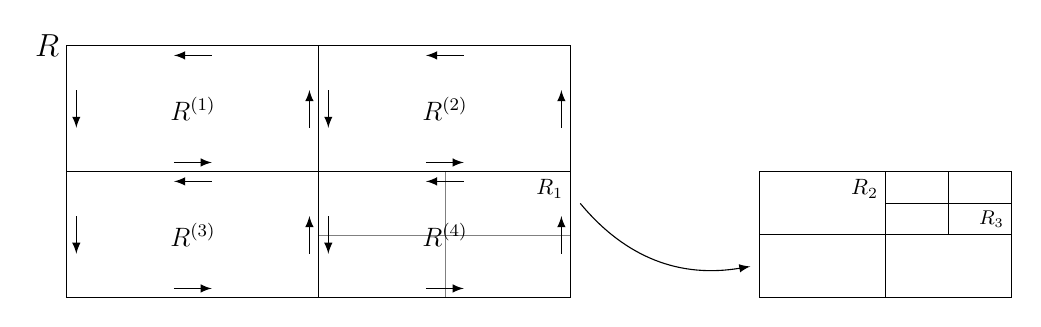
\begin{tikzpicture} [>=latex, scale=0.8, transform shape]
	\draw [help lines] (6,0) -- (6,2) (4,1) -- (8,1);
	\draw (0,0) rectangle (8,4);
	\draw (4,0) -- (4,4) (0,2) -- (8,2);
	\draw [->] (0.15,3.30) -- (0.15,2.70);
	\draw [->] (0.15,1.30) -- (0.15,0.70);
	\draw [->] (1.70,0.15) -- (2.30,0.15);
	\draw [->] (5.70,0.15) -- (6.30,0.15);
	\draw [<-] (7.85,3.30) -- (7.85,2.70);
	\draw [<-] (7.85,1.30) -- (7.85,0.70);
	\draw [<-] (1.70,3.85) -- (2.30,3.85);
	\draw [<-] (5.70,3.85) -- (6.30,3.85);
	\draw [->] (1.70,2.15) -- (2.30,2.15);
	\draw [->] (5.70,2.15) -- (6.30,2.15);
	\draw [<-] (1.70,1.85) -- (2.30,1.85);
	\draw [<-] (5.70,1.85) -- (6.30,1.85);
	\draw [->] (4.15,3.30) -- (4.15,2.70);
	\draw [->] (4.15,1.30) -- (4.15,0.70);
	\draw [<-] (3.85,3.30) -- (3.85,2.70);
	\draw [<-] (3.85,1.30) -- (3.85,0.70);
	\node [font=\large] at (2,3) {\(R^{(1)}\)};
	\node [font=\large] at (6,3) {\(R^{(2)}\)};
	\node [font=\large] at (2,1) {\(R^{(3)}\)};
	\node [font=\large] at (6,1) {\(R^{(4)}\)};
	\node [left, font=\Large] at (0,4) {\(R\)};
	\node [below left] at (8,2) {\(R_1\)};
	\draw [->] (8.15,1.5) to [bend right=30] (10.85,0.5);
	\draw (11,0) rectangle (15,2);
	\draw (13,0) -- (13,2) (11,1) -- (15,1);
	\draw (14,1) -- (14,2) (13,1.5) -- (15,1.5);
	\node [below left] at (13,2) {\(R_2\)};
	\node [above left, font=\small] at (15,1) {\(R_3\)};
\end{tikzpicture}
	\caption{Bisezione del rettangolo \(R\).}
	\label{fig:teorCauchyRettangolo}
\end{figure}

\begin{proof}
	Possiamo supporre che \(f\) sia olomorfa in un aperto che contiene \(R\). Infatti se prendo \(R_n \subseteq \mathring{R}\) con \(R_n \to R\), avrò che \(f\) è olomorfa in un aperto che contiene \(R_n\).
	Per il lemma precedente avremo
	\[
		\int\limits_{\pd R_n}f(z)\,\dd z = 0,\,\fa n \implies \int\limits_{\pd R}f(z)\,\dd z =0.
	\]
	Introduciamo la notazione
	\[
		\h(R) = \int\limits_{\pd R}f(z)\,\dd z,
	\]
	che utilizzeremo anche per ogni rettangolo contenuto in quello di partenza.
	Se dividiamo \(R\) in quattro rettangoli congruenti \(R^{(1)},R^{(2)},R^{(3)},R^{(4)}\), otteniamo che
	\[
		\h(R) = \h(R^{(1)})+\h(R^{(2)})+\h(R^{(3)})+\h(R^{(4)}),
	\]
	dal momento che, come è visibile nella \autoref{fig:teorCauchyRettangolo}, gli integrali si cancellano a vicenda sulle linee in comune.
	Applicando la triangolare avremo
	\[
		\abs{\h(R)} = \abs{\h(R^{(1)})+\h(R^{(2)})+\h(R^{(3)})+\h(R^{(4)})} \le \abs{\h(R^{(1)})}+\abs{\h(R^{(2)})}+\abs{\h(R^{(3)})}+\abs{\h(R^{(4)})},
	\]
	per cui almeno uno dei rettangoli \(R^{(k)}\), \(k=1,2,3,4\), soddisferà la condizione
	\[
		\abs{\h(R^{(k)})} \ge \frac{1}{4}\abs{\h(R)}.
	\]
	Chiamiamo tale rettangolo \(R_1\).
	Iterando questo processo otteniamo una catena di rettangoli \(R\supset R_1 \supset \ldots \supset R_n \supset ...\) con la proprietà
	\[
		\abs{\h(R_n)} \ge \frac{1}{4}\abs{\h(R_{n-1})} \implies \abs{\h(R_n)} \ge \frac{1}{4^n}\abs{\h(R)}.
	\]
	Poiché la catena di rettangoli è in particolare una catena di compatti, la loro intersezione convergerà ad un punto \(z^*\in R\), ovvero \(R_n\) sarà contenuto in un intorno \(D(z^*,\d)\) quando \(n\) sarà sufficientemente grande.
	Possiamo inoltre prendere \(\d\) abbastanza piccolo affinché \(f\) sia definita e olomorfa in \(D(z^*,\d)\).
	Inoltre, fissato \(\e>0\), possiamo trovare \(\d\) tale che
	\[
		\abs*{\frac{f(z)-f(z^*)}{z-z^*}-f'(z^*)} \le \e \qquad\text{se }\abs{z-z^*}<\d,
	\]
	ovvero
	\begin{equation}\label{eq:teorCauchyRettangoli}
		\abs{f(z)-f(z^*)-f'(z^*)(z-z^*)} \le \e\abs{z-z^*} \qquad\text{se }\abs{z-z^*}<\d.
	\end{equation}
	Assumiamo quindi che \(\d\) soddisfi queste condizioni e che \(R_n\) sia contenuto in \(D(z^*,\d)\).
	Osserviamo inoltre che
	\[
		\int\limits_{\pd R_n} \dd z = 0 \qquad\text{e}\qquad \int\limits_{\pd R_n} z\,\dd z = 0.
	\]
	Questi casi particolari sono banalmente veri in quanto \(1\) e \(z\) sono rispettivamente le derivate di \(z\) e \(z^2/2\) e \(\pd R_n\) è una curva chiusa.

	Di conseguenza possiamo scrivere
	\[
		\h(R_n) = \int\limits_{\pd R_n} f(z)\,\dd z = \int\limits_{\pd R_n} \big[f(z)-f(z^*)-f'(z^*)(z-z^*)\big]\,\dd z,
	\]
	da cui, per la \eqref{eq:teorCauchyRettangoli}
	\[
		\abs{\h(R_n)} \le \int\limits_{\pd R_n} \e\,\abs{z-z^*}\,\abs{\dd z}.
	\]
	Nell'ultimo integrale \(\abs{z-z^*}\) è al più uguale al diametro \(D_n\) di \(R_n\).
	Inoltre, se denotiamo con \(P_n\) il perimetro di \(R_n\), otteniamo
	\[
		\abs{\h(R_n)} \le \e\,D_n\,\int\limits_{\pd R_n} \abs{\dd z} = \e\,D_n P_n.
	\]
	D'altronde se \(D\) e \(P\) sono rispettivamente il diametro e il perimetro del rettangolo \(R\) di partenza, valgono
	\[
		D_n = \frac{D}{2^n} \qquad\text{e}\qquad P_n = \frac{P}{2^n},
	\]
	da cui
	\[
		\abs{\h(R_n)} \le \frac{\e\,D\,P}{4^n} \implies \abs{\h(R)} \le \e\,D\,P.
	\]
	Dal momento che \(\e\) è arbitrario possiamo solamente avere \(\h(R)=0\), ovvero la tesi.
\end{proof}

\begin{teor}{di Cauchy per i dischi aperti}{teorCauchyDischi}\index{Teorema di Cauchy!per i dischi aperti}
	Siano \(D\subseteq\C\) un disco aperto e \(z_0\) il centro di \(D\).
	Sia \(f\colon D \to \C\) olomorfa in \(D\).
	Se \(\g\colon [a,b] \to D\) è una curva chiusa di classe \(C^1\), allora
	\[
		\int\limits_\g f(z)\,\dd z = 0.
	\]
\end{teor}

\begin{figure}[tp]
	\centering
	\begin{tikzpicture}[>=To]
	\coordinate [label={[font=\large]below left:\(z_0\)}] (A) at (0,0);
	\coordinate (B) at (3,0);
	\coordinate (C) at (5,0);
	\coordinate (D) at (5,3);
	\coordinate [label={[font=\large]left:\(z\)}] (E) at (3,3);
	\coordinate [label={[font=\large]right:\(z+h\)}] (F) at (5,5);

	\draw [->-] (A) -- (B);
	\draw [->-] (B) -- (C);
	\draw [->-] (C) -- (D);
	\draw [->-, very thick] (D) -- (F);
	\draw [->-] (B) -- (E);
	\draw [->-, very thick] (E) -- (D);
	\draw (E) -- (F);

	\node [above=0.1cm] at ($(A)!0.5!(B)$) {\(\g_1\)};
	\node [left=0.1cm] at ($(B)!0.5!(E)$) {\(\g_2\)};
	\node [above=0.1cm] at ($(B)!0.5!(C)$) {\(\g_3\)};
	\node [right=0.1cm] at ($(C)!0.5!(D)$) {\(\g_4\)};
	\node [right=0.1cm] at ($(D)!0.5!(F)$) {\(\g_5\)};
	\node [below=0.1cm] at ($(D)!0.5!(E)$) {\(\g_6\)};
\end{tikzpicture}
	\caption{Curve per \(F(z+h)-F(z)\).}
	\label{fig:teorCacuhyDisco}
\end{figure}

\begin{proof}
	Per la \autoref{pr:integraleDerivataContinua} è sufficiente trovare \(F\colon D \to \C\) olomorfa tale che \(F'(z)=f(z),\,\fa z\in D\).
	Definisco quindi
	\[
		F(z) = \int\limits_{\g_1} f(w)\,\dd w + \int\limits_{\g_2} f(w)\,\dd w,
	\]
	dove \(\g_1\) consiste nella curva orizzontale da \((x_0,y_0)\) a \((x,y_0)\) e \(\g_2\) in quella verticale da \((x,y_0)\) a \((x,y)\).

	Per mostrare che \(F\) è olomorfa e vale \(F'(z)=f(z)\), per prima cosa mostriamo \(F'(z_0)=f(z_0)\), verificandolo con la definizione di derivata.
	Posto \(h=z-z_0\) avremo
	\[
		\begin{split}
			\bigg\lvert\frac{1}{h}\big[F(z)-\cancel{F(z_0)}-f(z_0)h\big]\bigg\rvert & = \bigg\lvert\frac{1}{h}\bigg[ \int\limits_{\g_1+\g_2}f(w)\,\dd w - f(z_0)h \bigg]\bigg\rvert = \bigg\lvert \frac{1}{h} \int\limits_{\g_1+\g_2}\big[f(w)-f(z_0)\big]\,\dd w \bigg\rvert\\
			& \le \frac{1}{\abs{h}} \int\limits_{\g_1+\g_2} \big\lvert f(w) - f(z_0) \big\rvert\,\abs{\dd w} \le \frac{\e}{\abs{h}} \int\limits_{\g_1+\g_2} \abs{\dd w}\graffito{\(\big\lvert f(w)-f(z_0)\big\rvert \le \e\) se \(\abs{h}<\d\)}\\
			& = \frac{\e}{\abs{h}}\,\sqrt{2}\abs{h} = \e \sqrt{2}
		\end{split}
	\]
	Per cui dato \(\e\) trovo \(\d\) tale che, per \(\abs{h}<\d\), si ha
	\[
		\bigg\lvert\frac{1}{h}\big[F(z)-F(z_0)-f(z_0)h\big]\bigg\rvert \le \e \implies F'(z_0) = f(z_0).
	\]
	Mostriamo adesso il caso generale:
	\[
		F(z+h)-F(z) = \int\limits_{\mathclap{\cancel{\g_1}+\g_3+\g_4+\g_5}}f(w)\,\dd w - \int\limits_{\mathclap{\cancel{\g_1}+\g_2}} f(w)\,\dd w,
	\]
	dove \(\g_1,\g_2,\g_3,\g_4,\g_5,\g_6\) sono le curve mostrate in \autoref{fig:teorCacuhyDisco}.
	Ora, il \hyperref[th:teorCauchyRettangoli]{teorema di Cauchy per i rettangoli} applicato al rettangolo identificato da \(\g_2+\g_6-\g_4-\g_3\) ci dice che l'integrale di \(f\) lungo il rettangolo è nullo, per cui
	\[
		\begin{split}
			F(z+h)-F(z) & = \int\limits_{\mathclap{\g_3+\g_4+\g_5}}\,f(w)\,\dd w - \int\limits_{\g_2}f(w)\,\dd w = \int\limits_{\mathclap{\g_3+\g_4+\g_5}}\,f(w)\,\dd w - \int\limits_{\g_2}f(w)\,\dd w + \int\limits_{\mathclap{\g_2+\g_6-\g_4-\g_3}}\,f(w)\,\dd w\\
			& = \int\limits_{\mathclap{\g_5+\g_6}}\,f(w)\,\dd w,
		\end{split}
	\]
	che è analogo al caso precedente.
\end{proof}
%!TEX root = ../main.tex
%%%%%%%%%%%%%%%%%%%%%%%%%%%%%%%%%%%%%%%%%
%
%LEZIONE 11/10/2016 - TERZA SETTIMANA (1)
%
%%%%%%%%%%%%%%%%%%%%%%%%%%%%%%%%%%%%%%%%%
%%%%%%%%%%%%%%%%%%%%%%%%%%%%%
%FORMULA INTEGRALE DI CAUCHY%
%%%%%%%%%%%%%%%%%%%%%%%%%%%%%
\chapter{Formula integrale di Cauchy}

Una semplice applicazione del teorema di Cauchy ci permette di rappresentare una funzione olomorfa come un integrale di linea. In questo capitolo studieremo le numerose conseguenze di tale formula.
%%%%%%%%%%%%%%
%INTRODUZIONE%
%%%%%%%%%%%%%%
\section{Introduzione}
\begin{teor}{Formula integrale di Cauchy}{formulaIntegraleCauchy}\index{Formula!integrale di Cauchy}
	Sia \(f\colon D(z_0;r) \to \C\) una funzione olomorfa e sia \(\g\) una curva chiusa in \(D(z_0;r)\setminus\{z_0\}\) tale che \(\ind(\g,z_0)=1\). Allora
	\[
		f(z_0) = \frac{1}{2\p\,i} \int\limits_\g \frac{f(z)}{z-z_0}\,\dd z.
	\]
\end{teor}

% \begin{figure}[tp]
% \centering
% 	\tikz[baseline=-0.5ex]{
	\draw [
		decoration={markings, mark=at position 0 with {\arrow{>}}},
		postaction={decorate},
		thick
		] (0,0) circle (1);
	\draw [thick] (0,0) circle (1.5);
	\fill (0,0) circle (0.02);
	\draw (0,0) -- (45:1);
	\node [below, font=\small] at (0,0) {\(z_0\)};
	\node [below right, font=\footnotesize] at (45:0.5) {\(r'\)};
	\fill (210:0.7) circle (0.02);
	\node [below, font=\small] at (210:0.7) {\(z\)};

	\node [above right] at (45:1.5) {\(D(z_0;r)\)};
	\node [below right] (A) at (-45:1.5) {\(D(z_0;r')\)};
	\draw [help lines] (-60:1.15) to [bend right] (A.west);
}
% 	\caption{}
% \end{figure}

\begin{proof}
	Definiamo la seguente funzione
	\[
		g(z) = 	\begin{cases}
			\frac{f(z)-f(z_0)}{z-z_0} & z\neq z_0 \\
			f'(z_0)                   & z=z_0
		\end{cases}
	\]
	tale funzione è continua in \(D(z_0;r)\) e inoltre è olomorfa in \(D(z_0;r)\) poiché quoziente di funzioni olomorfe e, \hyperref[th:teoremaSingolaritàEliminabile]{come vedremo in seguito}, \(z_0\) è una singolrità eliminabile.
	Applicando il \hyperref[th:teorCauchyDischi]{teorema di Cauchy} otteniamo
	\[
		\begin{split}
			0 & = \int\limits_\g \frac{f(z)-f(z_0)}{z-z_0}\,\dd z = \int\limits_\g \frac{f(z)}{z-z_0}\,\dd z - f(z_0)\,\int\limits_\g \frac{\dd z}{z-z_0}\\
			& = \int\limits_\g \frac{f(z)}{z-z_0}\,\dd z - f(z_0)\,2\p\,i\,\underbrace{\ind(\g,z_0)}_{=1},
		\end{split}
	\]
	da cui
	\[
		f(z_0) = \frac{1}{2\p\,i}\int\limits_\g \frac{f(z)}{z-z_0}\,\dd z. \qedhere
	\]
\end{proof}

\begin{oss}
	In generale quindi il valore di \(f\) in un aperto è determinato dal valore di \(f\) sul bordo dell'aperto. Da ciò segue che preso \(r'<r\), ho che, se \(z\in D(z_0;r')\), allora
	\[
		f(z) = \frac{1}{2\p\,i} \int\limits_{\mathclap{\pd B(z_0;r')}} \frac{f(w)}{w-z}\,\dd w \qquad\qquad \tikz[baseline=-0.5ex]{
	\draw [
		decoration={markings, mark=at position 0 with {\arrow{>}}},
		postaction={decorate},
		thick
		] (0,0) circle (1);
	\draw [thick] (0,0) circle (1.5);
	\fill (0,0) circle (0.02);
	\draw (0,0) -- (45:1);
	\node [below, font=\small] at (0,0) {\(z_0\)};
	\node [below right, font=\footnotesize] at (45:0.5) {\(r'\)};
	\fill (210:0.7) circle (0.02);
	\node [below, font=\small] at (210:0.7) {\(z\)};

	\node [above right] at (45:1.5) {\(D(z_0;r)\)};
	\node [below right] (A) at (-45:1.5) {\(D(z_0;r')\)};
	\draw [help lines] (-60:1.15) to [bend right] (A.west);
}
	\]
\end{oss}

\begin{oss}
	Esistono funzioni \(C^{\infty}(\R,\R)\), dette modificatori, che sono nulle fuori da un compatto, ad esempio
	\[
		f(x) = 	\begin{cases}
			e^{-\frac{1}{{(\abs{x}^2-1)}^2}} & x\in(-1,1)        \\
			0                                & \text{altrimenti}
		\end{cases}
	\]
	Se fosse possibile replicare questo comportamento in \(\R^2 \to \R^2\) avremmo trovato un controesempio al teorema. Da ciò deduciamo che non esistono modificatori olomorfi, ovvero non esistono funzioni olomorfe nulle fuori da un compatto.
\end{oss}

\begin{ese}
	Calcoliamo il seguente integrale
	\[
		\int\limits_{\abs{z}=1} \frac{e^z}{z}\,\dd z.
	\]
	Se prendo \(f(z)=e^z\), applicando la formula di Cauchy nell'origine ottengo
	\[
		1=f(0) = \frac{1}{2\p\,i} \int\limits_{\abs{z}=1} \frac{e^z}{z}\,\dd z.
	\]
	Per cui il nostro integrale vale \(2\p\,i\).
\end{ese}

\begin{ese}
	Calcoliamo il seguente integrale
	\[
		\int\limits_{\abs{z}=2} \frac{\dd z}{z^2+1}.
	\]
	Applichiamo qualche manipolazione
	\[
		\int\limits_{\abs{z}=2} \frac{\dd z}{z^2+1} = \int\limits_{\abs{z}=2} \frac{1}{2i} \left( \frac{1}{z-i}-\frac{1}{z+i} \right)\,\dd z = \frac{1}{2i} \bigg[ \int\limits_{\abs{z}=2} \frac{1}{z-i}\,\dd z - \int\limits_{\abs{z}=2} \frac{1}{z+i}\,\dd z\bigg],
	\]
	che è la formula di Cauchy applicata a \(f(z)=1\), da cui
	\[
		\int\limits_{\abs{z}=2} \frac{\dd z}{z^2+1} = \p\,(1-1) = 0.
	\]
\end{ese}
%%%%%%%%%%%%%%%%%%%%
%DERIVATE SUPERIORI%
%%%%%%%%%%%%%%%%%%%%
\section{Derivate superiori}

\begin{pr}
	Le serie di potenze sono olomorfe all'interno del disco di convergenza.
\end{pr}

\begin{proof}
	Supponiamo che \(f\) sia una serie di potenze del tipo
	\[
		f(z) = \sum_{n\ge 0}a_n (z-z_0)^n.
	\]
	\(f\) converge uniformemente sui compatti di \(D(z_0;r)\) dove \(r\) è il suo raggio di convergenza. Ora la serie delle derivate
	\[
		\sum_{n\ge 1}n\,a_n (z-z_0)^{n-1},
	\]
	converge ancora uniformemente sui compatti di \(D(z_0;r)\).
	D'altronde se la serie delle derivate converge uniformemente e la serie delle funzioni converge in un punto, allora la serie delle funzioni converge in un punto e la derivata della serie è la serie delle derivate.
\end{proof}

\begin{oss}
	In generale ciò significa che le serie di potenze possono essere derivate termine a termine.
\end{oss}

\begin{ese}
	Consideriamo la funzione esponenziale
	\[
		f(z) = e^z = \sum_{n\ge 0} \frac{z^n}{n!},
	\]
	che ha raggio di convergenza \(+\infty\). \(f\) è quindi una funzione intera.
	Scriviamo ora la sua derivata
	\[
		\frac{\dd}{\dd z}e^z = \sum_{n\ge 1}\frac{n}{n!}z^{n-1} = \sum_{n\ge 1}\frac{z^{n-1}}{(n-1)!} = \sum_{k\ge 0}\frac{z^k}{k!} =e^z.
	\]
\end{ese}

\begin{teor}{Funzioni olomorfe sono analitiche}{funzioniOlomorfeAnalitiche}\index{Teorema!delle funzioni analitiche}
	Sia \(\Omega \subseteq \C\) aperto e sia \(f\colon \Omega \to \C\) una funzione olomorfa. Preso \(z_0\in\Omega\) sia \(D(z_0;r)\) il più grande disco centrato in \(z_0\) e contenuto in \(\Omega\).
	Allora per ogni \(z\in D(z_0;r)\) si ha
	\[
		f(z) = \sum_{n\ge 0}a_n (z-z_0)^n, \qquad\text{con }a_n = \frac{1}{2\p\,i}\int\limits_\g \frac{f(z)}{(z-z_0)^{n+1}}\,\dd z,
	\]
	dove \(\g=\pd D(z_0;r')\) con \(r'<r\).
\end{teor}

\begin{proof}
	Applicando il \hyperref[th:teorCauchyRettangoli]{teorema di Cauchy} ad \(f\) otteniamo
	\[
		\begin{split}
			f(z) & = \frac{1}{2\p\,i} \int\limits_\g \frac{f(w)}{w-z}\,\dd w = \frac{1}{2\p\,i} \int\limits_\g \frac{f(w)}{(w-z_0)-(z-z_0)}\,\dd w\\
			& = \frac{1}{2\p\,i} \int\limits_\g \frac{1}{w-z_0}f(w) \frac{\dd w}{1- \frac{z-z_0}{w-z_0}} = \frac{1}{2\p\,i} \int\limits_\g \frac{f(w)}{w-z_0} \sum_{n\ge 0} \frac{(z-z_0)^n}{(w-z_0)^n}\,\dd w\graffito{utilizzo la serie geometrica}\\
			& = \frac{1}{2\p\,i} \int\limits_\g f(w) \sum_{n\ge 0}\frac{(z-z_0)^n}{(w-z_0)^{n+1}}\,\dd w,
		\end{split}
	\]
	dove la serie converge uniformemente in \(w\) in quanto
	\[
		\frac{\abs{z-z_0}}{\abs{w-z_0}} = \frac{\abs{z-z_0}}{r'} < \frac{r'}{r'} = 1.
	\]
	Posso quindi portare la serie fuori dall'integrale ottenendo
	\[
		f(z) = \frac{1}{2\p\,i} \sum_{n\ge 0} \int\limits_\g \frac{f(w)}{(w-z_0)^{n+1}}\,\dd w (z-z_0)^n = \sum_{n\ge 0}a_n (z-z_0)^n.\qedhere
	\]
\end{proof}

\begin{oss}
	Avremmo anche potuto dimostrare che
	\[
		f^{(n)}(z_0) = \frac{n!}{2\p\,i} \int\limits_\g \frac{f(w)}{(w-z_0)^{n+1}}\,\dd w,
	\]
	per ottenere la tesi tramite l'espansione di Taylor.
\end{oss}

\begin{ese}
	Calcoliamo
	\[
		\int\limits_\g \frac{\dd z}{z^3(z^{10}-2)}, \qquad\text{dove }\g(t)=e^{i\,t}, t\in[0,2\p].
	\]
	Poniamo \(g(z)=\frac{1}{z^{10}-2}\) che risulta olomorfa in \(B(0;1+\e)\). Applicando la formula di Cauchy per le derivate avremo
	\[
		\frac{1}{2\p\,i} \int\limits_\g \frac{g(z)}{z^3}\,\dd z = \frac{g''(0)}{2!}.
	\]
	Poiché ci troviamo in \(B(0,1+\e)\) riusciamo facilmente a scrivere l'espansione di Taylor di \(g\) nell'origine, così da non dover calcolare esplicitamente la derivata seconda di \(g\).
	\[
		\frac{1}{z^{10}-2} = -\frac{1}{2-z^{10}} = -\frac{1}{2} \frac{1}{1- \left( \frac{z}{2^{1/10}} \right)^{10}} = -\frac{1}{2}\sum_{n\ge 0} \left( \frac{z}{\sqrt[10]{2}} \right)^{10 n}.
	\]
	Da cui segue \(g''(0)=0\).
\end{ese}

\begin{oss}
	Dal teorema segue che la serie di Taylor converge nel più grande disco \(D(z_0;r)\) contenuto in \(\Omega\).
\end{oss}

\begin{ese}
	Consideriamo, su \(\Omega=\C\setminus\{1\}\), la funzione
	\[
		f(z)= \frac{1}{1-z}.
	\]
	Sappiamo che la sua serie di Taylor è la segunte
	\[
		f(z) = \sum_{n\ge 0} z^n,\qquad \tikz[baseline=-0.5ex] {
	\draw [fill=contrast!10] (0,0) circle (1);
	\node [above left] at (2.1,0) {\(\R\)};
	\node [below right] at (0,2.1) {\(i\,\R\)};
	\draw [-latex, thick] (-1.2,0) -- (2.2,0);
	\draw [-latex, thick] (0,-1.2) -- (0,2.2);

	%\draw [pattern=north east lines wide] (0,0) circle (1);
	\node [below left, font=\footnotesize] at (-1,0) {\(-1\)};
	\node [below right, font=\footnotesize] at (1,0) {\(1\)};
}
	\]
	per cui otteniamo proprio che il suo raggio di convergenza è \(1\), come ci aspettavamo.
\end{ese}

\begin{teor}{di Liouville}{teoremaLiouville}\index{Teorema!di Liouville}
	Se \(f\colon \C \to \C\) è una funzione limitata e olomorfa, allora \(f\) è costante.
\end{teor}

\begin{proof}
	Basta dimostrare che \(f'(z)=0,\,\fa z\in \C\). Usiamo Cauchy per scrivere la derivata prima: posto \(\g=\pd D(z;r)\) avremo
	\[
		f'(z) = \frac{1}{2\p\,i} \int\limits_\g \frac{f(w)}{(w-z)^2}\,\dd w.
	\]
	Per ipotesi sappiamo \(\abs{f(w)}\le M\) per qualche \(M\in \R\). Da cui
	\[
		\begin{split}
			\abs{f'(z)} & \le \frac{1}{2\p} \int\limits_\g \frac{\abs{f(w)}}{\abs{w-z}^2}\,\abs{\dd w} = \frac{1}{2\p}\int\limits_\g \frac{\abs{f(w)}}{r^2}\,\abs{\dd w}\graffito{\(\abs{w-z}=r\) in quanto \(w\in \pd D(z;r)\)} \le \frac{1}{2\p}\int\limits_\g \frac{M}{r^2}\,\abs{\dd w}\\
			& = \frac{1}{2\p}\frac{M}{r^2}2\p\,r = \frac{M}{r} \xrightarrow{r\to \infty} 0,
		\end{split}
	\]
	da cui
	\[
		\abs{f'(z)}= 0,\,\fa z\in \C.\qedhere
	\]
\end{proof}

\begin{oss}
	In \(\R\) questo teorema è falso, si veda il seno come esempio di una funzione limitata che non è costante.
	D'altronde in \(\C\) il seno non è limitato, infatti
	\[
		\sin z = \frac{e^{i\,z}-e^{-i\,z}}{2\,i} \implies \sin(i\,t) = \frac{\sinh t}{i} \simeq e^{\abs{t}} \qquad\text{se \(t\) è grande}.
	\]
\end{oss}

\begin{ese}
	Supponiamo che \(f\colon \C \to \C\) sia olomorfa e tale che \(\abs{f(z)}\le \abs{e^z}\), dimostriamo che \(f(z)=a\,e^z\) per qualche \(a\) con \(\abs{a}<1\). Consideriamo
	\[
		g(z) = \frac{f(z)}{e^z}.
	\]
	Per ipotesi avremo
	\[
		\abs{g(z)} = \frac{\abs{f(z)}}{\abs{e^z}} \le 1.
	\]
	Quindi per il teorema di Liouville avremo \(g(z)\equiv a\), da cui \(f(z)=a\,e^z\).
\end{ese}

\begin{cor}
	Teorema Fondamentale dell'Algebra.
\end{cor}

\begin{proof}
	Il teorema di Liouville porta ad una semplice dimostrazione del Teorema Fondamentale dell'Algebra.
	Infatti se, preso \(P\colon \C \to \C\) con \(\deg P>0\), supponiamo per assurdo che \(P\) non abbia zeri, posso considerare la funzione
	\[
		g(z) = \frac{1}{P(z)},
	\]
	che è intera. Inoltre è limitata per Weierstrass generalizzato, infatti
	\[
		\lim_{\abs{z}\to +\infty} \abs{g(z)} = \lim_{\abs{z}\to+\infty} \frac{1}{\abs{a_n z^n+\ldots+a_0}} = 0.
	\]
	Quindi per il teorema di Liouville \(P\) risulta costante, ovvero un polinomio di grado \(0\), che è assurdo per ipotesi.
\end{proof}
%%%%%%%%%%%%%%%%%%%%%%%%%%%%%%%%%%%%%%%%%
%
%LEZIONE 14/10/2016 - TERZA SETTIMANA (2)
%
%%%%%%%%%%%%%%%%%%%%%%%%%%%%%%%%%%%%%%%%%
\begin{cor}
	Se \(f\colon \C \to \C\) è una funzione olomorfa tale che \(\Re(f)\) oppure \(\Im(f)\) è limitata, allora \(f\) è costante.
\end{cor}

\begin{proof}
	Supponiamo che \(\Re(f)\) sia limitata, ovvero esiste \(M>0\) tale che \(\abs{\Re f(z)}\le M,\,\fa z\in \C\).
	Consideriamo la funzione \(g(z)=e^{f(z)}\) che è intera. Inoltre avremo
	\[
		\abs{g(z)} = \abs{e^{\Re f(z)}e^{i\,\Im f(z)}} = e^{\Re f(z)} \le e^M.
	\]
	Quindi per il teorema di Liouville avremo \(g\) costante, da cui
	\[
		0 = g'(z) = \underbrace{e^{f(z)}}_{\neq 0}f'(z) \implies f'(z)= 0,\,\fa z\in\C,
	\]
	ovvero \(f\) costante.
\end{proof}

\begin{teor}{di Liouville generalizzato}{teoremaLiouvilleGeneralizzato}
	Sia \(f\colon \C \to \C\) una funzione olomorfa tale che
	\[
		\abs{f(z)} \le A + B\abs{z}^n,\,\fa z\in\C,
	\]
	allora \(f\) è un polinomio di grado al più \(n\).
\end{teor}

\begin{proof}
	Dimostriamo che \(f^{(n+1)}\equiv 0\) utilizzando la formula di Cauchy:
	\[
		f^{(n+1)}(z) = \frac{1}{2\p\,i}\int\limits_{\g_R} \frac{f(w)}{(w-z)^{n+2}}\,\dd w, \qquad\text{con } \g_R\colon [0,2\p] \to \C, t\mapsto z+R\,e^{i\,t}.
	\]
	Passando al modulo avremo
	\[
		\begin{split}
			\abs{f^{(n+1)}(z)} & = \frac{1}{2\p} \bigg\lvert \int_0^{2\p} \frac{f\big(z+R\,e^{i\,t}\big)}{(R\,e^{i\,t})^{n+2}}\,R\,i\,e^{i\,t}\,\dd t\bigg\rvert\\
			& \le \frac{1}{2\p} \int_0^{2\p} \frac{A+B\,\abs{z+R\,e^{i\,t}}^n}{R^{n+2}}\,R\,\dd t.
		\end{split}
	\]
	Osserviamo che l'argomento dell'integrale tende uniformemente a zero quando \(R\to+\infty\).
	Per la convergenza uniforme posso portare fuori il limite dall'integrale per ottenere che \(\abs{f^{(n+1)}(z)}\le 0\) quando \(R\to+\infty\), ovvero
	\[
		f^{(n+1)}(z) = 0,\,\fa z\in \C.\qedhere
	\]
\end{proof}

\begin{ese}
	Su \(\R\) questo teorema è falso, ad esempio la funzione \(f(x)=x^2+e^{-x^2}\) cresce in modo polinomiale ma non è un polinomio.
\end{ese}

\begin{teor}{di Morera}{teoremaMorera}\index{Teorema!di Morera}
	Sia \(\Omega\subseteq \C\) aperto e sia \(f\colon \Omega \to \C\) una funzione continua tale che, per ogni curva chiusa \(\g\) in \(\Omega\), si abbia
	\[
		\int\limits_\g f(z)\,\dd z = 0.
	\]
	Allora \(f\) è olomorfa in \(\Omega\).
\end{teor}

\begin{proof}
	Fissato \(z_0\in\Omega\) definiamo
	\[
		F(z) = \int\limits_{\g_z}f(w)\,\dd w,
	\]
	dove \(\g_z\) soddisfa \(\g_z(0)=z_0,\g_z(1)=z\).
	Osserviamo che \(F\) così definito non dipende dalla curva, infatti se \(\tilde{\g}\) è un'altra curva che soddisfa \(0\mapsto z_0,1\mapsto z\), definisco
	\[
		\hat{\g}(t) = 	\begin{cases}
			\g_z(t)         & t\in[0,1] \\
			\tilde{\g}(2-t) & t\in[1,2]
		\end{cases}
	\]
	che è una curva chiusa su \(\Omega\), quindi per ipotesi
	\[
		0 = \int\limits_{\hat{\g}} f(w)\,\dd w = \int\limits_{\g_z}f(w)\,\dd w - \int\limits_{\tilde{\g}}f(w)\,\dd w.
	\]
	A questo punto è sufficiente mostrare che \(F'(z)=f(z)\), infatti è facile dimostrare che
	\[
		F(z+h)-F(z) = \int\limits_{\g_h}f(w)\,\dd w \simeq f(z)\,h.
	\]
	Quindi \(f\) è la derivata di una funzione olomorfa, pertanto \(f\) è anch'essa olomorfa.
\end{proof}
%%%%%%%%%%%
%APPENDICE%
%%%%%%%%%%%
\section{Appendice}

\begin{teor}{Proprietà del valor medio}{valorMedio}\index{Proprietà del valor medio}
	Sia \(\Omega \subseteq \C\) aperto e sia \(f\colon \Omega \to \C\) una funzione olomorfa.
	Prendiamo \(z_0\in\Omega\) e \(r>0\) tale che \(D(z_0;r)\subseteq\Omega\), allora
	\[
		f(z_0) = \frac{1}{2\p} \int_0^{2\p} f(z_0+r\,e^{i\,\q})\,\dd \q.
	\]
\end{teor}

\begin{proof}
	Per la \hyperref[th:formulaIntegraleCauchy]{formula di Cauchy} sappiamo
	\[
		f(z_0) = \frac{1}{2\p\,i} \int\limits_{\pd D(z_0;r)} \frac{f(w)}{w-z_0}\,\dd w.
	\]
	Parametrizziamo \(\pd D(z_0;r)\) tramite \(\g_r\colon [0,2\p] \to \Omega, \q \mapsto z_0+r\,e^{i\,\q}\), da cui
	\[
		\begin{split}
			f(z_0) & =  \frac{1}{2\p\,i} \int\limits_{\g_r} \frac{f(w)}{w-z_0}\,\dd w = \frac{1}{2\p\,i} \int_0^{2\p} \frac{f(z_0+r\,e^{i\,\q})}{r\,e^{i\,\q}}\,r\,i\,e^{i\,\q}\,\dd \q\\
			& = \frac{1}{2\p} \int_0^{2\p} f(z_0+r\,e^{i\,\q})\,\dd \q.\qedhere
		\end{split}
	\]
\end{proof}

\begin{teor}{Principio del massimo modulo}{teoremaMassimoModulo}\index{Principio del massimo}
	Sia \(\Omega\subseteq \C\) aperto e connesso e sia \(f\colon \Omega \to \C\) una funzione olomorfa.
	Allora \(\abs{f}\) non può assumere massimo in \(z_0\in\Omega\) a meno che \(f\) non sia costante.
\end{teor}

\begin{proof}
	Supponiamo che \(\abs{f(z_0)}=\sup\Set{\abs{f(z)}:z\in\Omega}\), mostriamo che \(f\) è costante.
	Per prima cosa mostriamo che \(\abs{f(z)}=\abs{f(z_0)},\,\fa z\in\Omega\) tramite un argomento topologico:
	Definiamo
	\[
		\Omega_1 = \Set{z\in\Omega : \abs{f(z)} < \abs{f(z_0)}} \qquad\text{e}\qquad \Omega_2 = \Set{z\in\Omega : \abs{f(z)}=\abs{f(z_0)}}.
	\]
	Chiaramente \(\Omega_1\cup\Omega_2 = \Omega\) e \(\Omega_1\cap\Omega_2 = \emptyset\), mostriamo che tali insiemi sono anche aperti:
	\begin{itemize}
		\item \(\Omega_1 = \abs{f}^{-1}\big(-\infty,\abs{f(z_0)}\big)\), dove \(\abs{f}\) è una funzione continua e \(\big(-\infty,\abs{f(z_0)}\big)\) è un intervallo aperto. Per cui \(\Omega_1\) è aperto in quanto controimmagine di un aperto tramite funzione continua.
		\item Preso \(z_1\in\Omega_2\) applico il teorema del valor medio:
		      \[
			      \abs{f(z_1)} = \bigg\lvert \frac{1}{2\p} \int_0^{2\p}f(z_1+r\,e^{i\,t})\,\dd t\bigg\rvert \le \frac{1}{2\p} \int_0^{2\p}\big\lvert f(z_1+r\,e^{i\,t})\big\rvert\,\dd t.
		      \]
		      Osserviamo che \(z_1\in\Omega_2 \implies \abs{f(z_1)}=\abs{f(z_0)}\) che è massimo. Quindi \(\abs{f(z_1+r\,e^{i\,t})}\le \abs{f(z_1)}\), inoltre se la disuguaglianza fosse stretta anche per un solo valore di \(t\) allora lo sarebbe, per continuità, su tutto un intervallo. Ma in tal caso il valore medio di \(\abs{f(z_1+r\,e^{i\,t})}\), a cui si riferisce l'integrale, sarebbe strettamente minore di \(\abs{f(z_1)}\), che contraddirebbe quanto affermato con il teorema del valor medio. Per cui
		      \[
			      \abs{f(z_1+r\,e^{i\,t})} = \abs{f(z_1)},\,\fa t \in [0,2\p].
		      \]
		      Ovvero \(\Omega_2\) è aperto poiché ogni punto di \(\Omega_2\) ha un intorno aperto contenuto in \(\Omega_2\).
	\end{itemize}
	Per connessione di \(\Omega\) avremo quindi \(\Omega_1=\emptyset\) oppure \(\Omega_2=\emptyset\). D'altronde \(z_0\in\Omega_2\) ci dice che \(\Omega_2 \neq \emptyset\). Ne segue \(\Omega_1=\emptyset \implies \Omega_2=\Omega\), ovvero \(\abs{f}\) costante.

	Mostriamo ora che \(\abs{f}\) costante implica \(f\) costante: se
	\[
		f(x,y) = u(x,y)+i\,v(x,y),
	\]
	definiamo \(F(x,y)=u^2(x,y)+v^2(x,y)=\abs{f}^2\) che è quindi costante. In particolare avremo
	\[
		0 = \begin{pmatrix}\pd_x F(x,y) & \pd_y F(x,y)\end{pmatrix} = \begin{pmatrix}2u(x,y) & 2v(x,y)\end{pmatrix}
		\begin{pmatrix}
			\pd_x u(x,y) & \pd_y u(x,y) \\
			\pd_x v(x,y) & \pd_y v(x,y)
		\end{pmatrix}
	\]
	abbiamo quindi
	\[
		u(x,y) = v(x,y) = 0 \qquad\text{oppure}\qquad f'(x,y)=0,
	\]
	in entrambi i casi \(f\) risulta costante.
\end{proof}
%%%%%%%%%%%%%%%%%%%%%%%%%%%%%%%%%%%%%%%%%%
%
%LEZIONE 18/10/2016 - QUARTA SETTIMANA (1)
%
%%%%%%%%%%%%%%%%%%%%%%%%%%%%%%%%%%%%%%%%%%
\begin{teor}{Principio di identità}{principioIdentità}\index{Principio di identità}
	Sia \(\Omega\subseteq\C\) un aperto connesso e siano \(f,g\colon \Omega \to \C\) due funzioni olomorfe.
	Se \(f(z_n)=g(z_n)\) e \(z_n \to z_0\in\Omega\), allora
	\[
		f(z)=g(z)\,\fa z \in \Omega.
	\]
\end{teor}

\begin{proof}
	Posto \(h(z)=f(z)-g(z)\), ci basta dimostrare che se \(h(z_n)=0\) e \(z_n\to z_0\in\Omega\) allora \(h(z)=0 \,\fa z\in\Omega\).
	Definiamo quindi i seguenti insiemi e procediamo con l'usuale argomento di connessione:
	\[
		\Omega_1 = \Set{z | z\text{ punto di accumulazione e }h(z)=0}
	\]
	e
	\[
		\Omega_2 = \Set{z | h(z)\neq 0 \text{ oppure \(z\) zero isolato di \(h\)}}.
	\]
	Chiaramente \(\Omega=\Omega_1\cup \Omega_2\) e \(\Omega_1 \cap \Omega_2=\emptyset\).
	Ci basta quindi dimostrare che \(\Omega_1,\Omega_2\) sono aperti affinché, per connessione, si abbia che uno dei due insiemi è vuoto. D'altronde \(z_0\in \Omega_1\) per ipotesi quindi \(\Omega_1 \neq \emptyset \implies \Omega_1=\Omega\) da cui la tesi.
	\begin{itemize}
		\item \(\Omega_2\) aperto: sia \(\bar{z}\in\Omega_2\); se \(h(\bar{z})\neq0\) per la permanenza del segno esiste \(r>0\) tale che
		      \[
			      h(z)\neq0 \,\fa z\in B(\bar{z};r),
		      \]
		      ovvero \(B(\bar{z};r)\subseteq \Omega_2\).
		      Se invece \(\bar{z}\) è uno zero isolato di \(h\) è tautologico dire che vi è un intorno di \(\bar{z}\) che non contiene zeri di \(h\), ovvero trovo \(r>0\) tale che
		      \[
			      h(z)\neq 0 \,\fa z\in B(z_0;r)\setminus\{z_0\},
		      \]
		      da cui \(B(z_0;r)\subseteq \Omega_2\).
		\item \(\Omega_1\) aperto: preso \(\bar{z}\in\Omega_1\) sviluppiamo \(h\) nella sua serie di Taylor attorno a \(\bar{z}\):
		      \[
			      h(z) = \sum_{n=0}^{\infty}a_n(z-\bar{z})^n \qquad\text{per }z\in B(\bar{z};r)
		      \]
		      Da \(h(\bar{z})=0\) segue \(a_0=0\), in particolare avremo
		      \[
			      h(z) = a_n(z-\bar{z})^n + a_{n+1}(z-\bar{z})^{n+1}+\ldots \qquad\text{per }n\ge 1.
		      \]
		      D'altronde se per assurdo esistesse \(n\) tale che \(a_n\neq 0\) si avrebbe, per \(z\neq \bar{z}\) e \(\abs{z-\bar{z}}<\e\),
		      \[
			      h(z) = a_n(z-\bar{z})^n + a_{n+1}(z-\bar{z})^{n+1}+\ldots = (z-\bar{z})^n \big[a_n+a_{n+1}(z-\bar{z})+\ldots\big] \neq 0,
		      \]
		      in quanto \((z-\bar{z})\neq 0\) e \(l(z):=\big[a_n+a_{n+1}(z-\bar{z})+\ldots\big]\) è olomorfa, in particolare continua, da cui
		      \[
			      \abs{l(z)} \ge \frac{1}{2}\abs{l(\bar{z})} = \frac{1}{2}\abs{a_n} \neq 0.
		      \]
		      Ma ciò è assurdo in quanto \(\bar{z}\) risulterebbe uno zero isolato di \(h\), contraddicendo l'assunto di \(\bar{z}\in\Omega_1\).
		      Per cui \(a_n=0,\,\fa n \implies f(z)=0,\,\fa z\in B(\bar(z);r)\), da cui la tesi.\qedhere
	\end{itemize}
\end{proof}

\begin{oss}
	Consideriamo la seguente funzione:
	\[
		f(x) = 	\begin{cases}
			0                  & x\le 0 \\
			e^{-\frac{1}{x^2}} & x>0
		\end{cases}
	\]
	Tale funzione è \(C^{\infty}(\R)\) ma non coincide con la sua serie di Taylor.
	Infatti la serie è identicamente nulla mentre la funzione è ben lontana dall'esserlo.

	In \(\C\) quindi \(f\) non è olomorfa per varie ragioni: la prima è che non coincide con la sua serie di Taylor, la seconda come conseguenza del principio di identità.
\end{oss}

\begin{oss}
	Il principio di identità è generalmente falso per le funzioni \(C^{\infty}(\R^2,\R^2)\). Consideriamo ad esempio
	\[
		f(x,y) \equiv (0,0) \qquad\text{e}\qquad g(x,y) = (y^2,0).
	\]
	Tali funzioni coincidono sull'asse \(x\) ma sono chiaramente distinte.
\end{oss}

\begin{defn}{Convergenza quasi uniforme}{convergenzaQuasiUniforme}\index{Convergenza!quasi uniforme}
	Sia \(\Omega\subseteq \C\) aperto e sia \(\{f_n\}_{n\ge 1}\subseteq C(\Omega)\).
	Si dice che \(f_n\) \emph{converge quasi uniformemente} a \(f\) se vi converge uniformemente su tutti i compatti di \(\Omega\).
\end{defn}

\begin{prop}{Convergenza quasi uniforme delle serie di potenze}{convergenzaQUSeriePotenze}
	Le serie di potenze convergono quasi uniformemente nel loro disco di convergenza.
\end{prop}

\begin{proof}
	Supponiamo che la seguente serie di potenze
	\[
		\sum_{n = 0}^\infty a_n z^n,
	\]
	converga su \(D(0;R)\) dove \(R\) è il suo raggio di convergenza.
	Sia \(K\subseteq D(0;R)\) compatto. Per compattezza \(K\subseteq D(0;R-\e)\) per un \(\e>0\).
	Andiamo a studiare la convergenza totale della serie su tale disco:
	\[
		\sum_{n=0}^\infty \sup_{z\in K} \abs{a_n z^n} \le \sum_{n=0}^\infty \abs{a_n}\abs{R-\e}^n
	\]
	di cui si può valutare la convergenza tramite il criterio della radice:
	\[
		\limsup \sqrt[n]{\abs{a_n}}\abs{R-\e} = \frac{\abs{R-\e}}{R} < 1.
	\]
	Quindi la serie converge totalmente e di conseguenza uniformemente su \(K\).
\end{proof}

\begin{ese}
	La serie
	\[
		\sum_{n=0}^N \frac{z^n}{n!}
	\]
	non converge uniformemente a \(e^z\) su \(\C\) dal momento che
	\[
		\norma*{\sum_{n=0}^N \frac{z^n}{n!}-e^z}_{\sup} = +\infty.
	\]
	D'altronde converge uniformemente sulle palle.
\end{ese}

\begin{teor}{Rigidità olomorfa sulla convergenza quasi uniforme}{rigiditàOlomorfaConvergenza}
	Sia \(\Omega\subseteq\C\) aperto e sia \(f_n\colon \Omega \to \C\) una funzione olomorfa per ogni \(n\).
	Se \(f_n \to f\) quasi uniformemente allora \(f\) è olomorfa.
\end{teor}

\begin{proof}
	Fissato \(z\in \Omega\), consideriamo \(\chius{B(z_0;r)}\subseteq \Omega\) e poniamo \(\g=\pd B(z_0;r)\).
	Per la formula di Cauchy avremo
	\[
		f_n(z) = \frac{1}{2\p\,i} \int\limits_\g \frac{f_n(w)}{w-z}\,\dd w.
	\]
	Osserviamo che \(\pd B(z_0;r)\) è compatto, quindi
	\[
		f_n(z) = \frac{1}{2\p\,i} \int\limits_\g \frac{f_n(w)}{w-z}\,\dd w \to \frac{1}{2\p\,i} \int\limits_\g \frac{f(w)}{w-z}\,\dd w
	\]
	poiché la convergenza uniforme mi permette di passare il limite nell'integrale di Riemann.
	Inoltre, per ipotesi, \(f_n(z) \to f(z)\), da cui, per l'unicità del limite,
	\[
		f(z)= \frac{1}{2\p\,i} \int\limits_\g \frac{f(w)}{w-z}\,\dd w \qquad\text{se }z\in B(z_0;r).
	\]
	Ciò significa che \(f\) è olomorfa per la differenziabilità sotto segno di integrale.
\end{proof}

\begin{oss}
	Inoltre si dimostra tramite la formula di Cauchy per le derivate superiori che
	\[
		f^{(k)}_n \to f^{(k)}
	\]
	quasi uniformemente in \(\Omega\).
\end{oss}
%!TEX root = ../main.tex
%%%%%%%%%%%%%%%%%%%%%%%%%%%%%%%%%%%%%%%%%%
%
%LEZIONE 18/10/2016 - QUARTA SETTIMANA (1)
%
%%%%%%%%%%%%%%%%%%%%%%%%%%%%%%%%%%%%%%%%%%
\chapter{Forma generale del teorema di Cauchy}

Ricordiamo che il \hyperref[teoremaCauchy]{teorema di Cauchy} affermava che se \(f\colon B(z_0;r)\to \C\) è una funzione olomorfa e \(\g\) è una curva chiusa in \(B(z_0;r)\), allora
\[
	\int\limits_\g f(z)\,\dd z = 0.
\]
Questo però non vale al di fuori delle palle, ad esempio per una funzione definita in un aperto non semplicemente connesso come
\[
	f\colon \Omega\setminus\{0\} \to \C, f(z) = \frac{1}{z},
\]
avevamo osservato che
\[
	\frac{1}{2\p\,i} \int\limits_{\g_1} \frac{\dd z}{z} = \ind(\g_1,0).
\]
D'altra parte se considerassimo una seconda curva \(\g_2\) all'interno di \(\g_1\), percorsa in senso contrario, troveremmo
\[
	\int\limits_{\mathclap{\g_1+\g_2}}\,\frac{\dd z}{z} = \int\limits_{\g_1}\frac{\dd z}{z} + \int\limits_{\g_2}\frac{\dd z}{z} = 1-1=0 \qquad\qquad
	\tikz[baseline=-0.5ex]{
	\draw [-latex, thick] (-1.6,0) -- (2,0);
	\draw [-latex, thick] (0,-1.6) -- (0,2);
	\draw [
		decoration={markings, mark=at position 0.125 with {\arrow{>}}},
		postaction={decorate}
		] (0,0) circle (1.5);
	\draw [
		decoration={markings, mark=at position 0.125 with {\arrow{<}}},
		postaction={decorate}
		] (0,0) circle (0.75);
	\draw [fill=white] (0,0) circle (0.1);

	\node [above left] at (2,0) {\(x\)};
	\node [below right] at (0,2) {\(y\)};
	\node [above right, font=\footnotesize] at (45:0.75) {\(\g_2\)};
	\node [above right, font=\footnotesize] at (45:1.5) {\(\g_1\)};
}
\]
In questo modo possiamo generalizzare il Teorema di Cauchy per domini non semplicemente connessi.
%%%%%%%%%%%%%%
%INTRODUZIONE%
%%%%%%%%%%%%%%
\section{Introduzione}

\begin{defn}{Catene e cicli}{cateneCiclie}\index{Catene}\index{Cicli}
	Se \(\g_1,\ldots,\g_n\) sono curve \(C^1\) e \(a_1,\ldots,a_n\in\Z\), definiamo la seguente somma formale
	\[
		a_1\g_1 + \ldots+ a_n\g_n
	\]
	come \emph{catena}. Se, inoltre, \(\g_1,\ldots,\g_n\) sono curve chiuse, la somma formale si chiama \emph{ciclo}.
\end{defn}

\begin{oss}
	Sappiamo già che possiamo considerare una curva come un elemento del duale delle funzioni continue su \(\C\). Per cui dalla definizione di catena segue
	\[
		\int\limits_{\mathclap{a_1\g_1+\ldots+a_n\g_n}}\,f(z)\,\dd z = a_1 \int\limits_{\g_1}f(z)\,\dd z + \ldots + a_n \int\limits_{\g_n} f(z)\,\dd z.
	\]
	Dove \(f\) è una funzione continua su \(\C\).
\end{oss}

\begin{teor}{Forma generale del teorema di Cauchy}{teorCauchyGenerale}\index{Teorema di Cauchy!generalizzato}
	Sia \(\Omega\subseteq\C\) un aperto qualsiasi e sia \(f\colon \Omega \to \C\) una funzione olomorfa.
	Sia \(\Gamma\) un ciclo tale che
	\[
		\ind(\Gamma,\a):= \frac{1}{2\p\,i} \int\limits_\Gamma \frac{\dd z}{z-\a} =0,\,\fa \a\not\in\Omega.
	\]
	Allora se \(z\not\in \im(\Gamma)\) si ha che
	\[
		f(z) \cdot \ind(\Gamma,z) = \frac{1}{2\p\,i} \int\limits_\Gamma \frac{f(w)}{w-z}\,\dd z \qquad\text{e}\qquad \int\limits_\Gamma f(z)\,\dd z = 0.
	\]
\end{teor}

\begin{proof}
	Non fornita ma analoga ai casi già discussi.
\end{proof}

\begin{ese}
	Sia \(\Gamma = \g_1+\g_2-\g_3\) come mostrato in figura. Consideriamo la seguente funzione
	\[
		f\colon \C\setminus\{0,1\} \to \C, z \mapsto \frac{1}{z\,(z-1)} \qquad\qquad \tikz[baseline=-0.5ex, x=2cm, y=2cm]{
	\draw [-latex, thick] (-0.9,0) -- (2,0);
	\draw [-latex, thick] (0,-0.7) -- (0,1);
	\draw [
		decoration={markings, mark=at position 0.125 with {\arrow{>}}},
		postaction={decorate}
		] (0,0) circle (0.3);
	\draw [
		decoration={markings, mark=at position 0.125 with {\arrow{>}}},
		postaction={decorate}
		] (1,0) circle (0.3);
	\draw [
		decoration={markings, mark=at position 0.25 with {\arrow{>}}},
		postaction={decorate}
		] (0.5,0) circle [x radius=1.2, y radius=0.6];
	\draw [fill=white] (0,0) circle (0.05);
	\draw [fill=white] (1,0) circle (0.05);

	\node [above left] at (2,0) {\(x\)};
	\node [below right] at (0,1) {\(y\)};
	\node [above right, font=\footnotesize] at ($(1,0)+(45:0.3)$) {\(\g_2\)};
	\node [above right, font=\footnotesize] at (45:0.3) {\(\g_1\)};
	\node [above right, font=\footnotesize] at (0.5,0.6) {\(\g_3\)};
	\node [below left, font=\scriptsize] at (0,0) {\(0\)};
	\node [below left, font=\scriptsize] at (1,0) {\(1\)};
}
	\]
	\(\Gamma\) soddisfa le ipotesi di Cauchy generalizzato, infatti
	\[
		\ind(\Gamma,0) = \frac{1}{2\p\,i} \int\limits_{\mathclap{\g_1+\g_2-\g_3}}\, \frac{\dd z}{z} = \frac{1}{2\p\,i} \bigg[ \int\limits_{\g_1}\frac{\dd z}{z} + \int\limits_{\g_2} \frac{\dd z}{z} - \int\limits_{\g_3}\frac{\dd z}{z}\bigg] = \frac{1}{2\p\,i}(1+0-1) = 0,
	\]
	analogamente si mostra \(\ind(\Gamma,1)=0\), da cui
	\[
		\int\limits_{\mathclap{\g_1+\g_2-\g_3}}\, \frac{\dd z}{z\,(z-1)} = 0.
	\]
\end{ese}
%%%%%%%%%%%%%%%%%%%%%%%%%%%%%%%%%%%%%%%%%%
%
%LEZIONE 21/10/2016 - QUARTA SETTIMANA (2)
%
%%%%%%%%%%%%%%%%%%%%%%%%%%%%%%%%%%%%%%%%%%
%%%%%%%%%%%%%%%%%%
%SERIE DI LAURENT%
%%%%%%%%%%%%%%%%%%
\section{Serie di Laurent}

\begin{defn}{Serie di Laurent}{serieLaurent}\index{Serie di Laurent}
	Una serie del tipo
	\[
		\sum_{n\in \Z}a_n(z-z_0)^n,
	\]
	si definisce \emph{serie di Laurent} centrata in \(z_0\in\C\).
\end{defn}

\begin{prop}{Convergenza della serie di Laurent}{convergenzaSerieLaurent}\index{Serie di Laurent!convergenza}
	Consideriamo una generica serie di Laurent \(\Sigma\) centrata in \(z_0\in\C\).
	Siano
	\[
		R = \frac{1}{\limsup_{n\to +\infty}\sqrt[n]{\abs{a_n}}} \qquad\text{e}\qquad r = \limsup_{n\to +\infty}\sqrt[n]{\abs{a_{-n}}}.
	\]
	Se \(r<R\) allora \(\Sigma\) converge in \(D(z_0;R)\setminus\chius{D(z_0;r)}\).
\end{prop}

\begin{proof}
	Supponiamo di scrivere
	\[
		\Sigma = \sum_{n\in\Z}a_n (z-z_0)^n.
	\]
	Se consideriamo solo i termini con indice positivo sappiamo che
	\[
		\sum_{n\ge 0} a_n (z-z_0)^n
	\]
	converge in \(D(z_0;R)\) dove \(R\) come definito nell'ipotesi è il suo raggio di convergenza.
	D'altronde se consideriamo i termini negativi
	\[
		\sum_{n\le 1} a_n (z-z_0)^n,
	\]
	avremo che tale serie converge se
	\[
		\frac{1}{\abs{z-z_0}} < \frac{1}{\limsup_{n\to +\infty}\sqrt[n]{\abs{a_n}}} \iff \abs{z-z_0} > r,
	\]
	ovvero in \(\C\setminus \chius{D(z_0;r)}\).

	Da ciò segue che \(\Sigma\) converge nell'intersezione dei due insiemi di convergenza, rispettivamente della serie con indici positivi e quella con indici negativi.
	In particolare se \(r<R\) tale intersezione è non vuota e \(\Sigma\) converge sulla corona \(D(z_0;R)\setminus \chius{D(z_0;r)}\).
\end{proof}

\begin{oss}\label{oss:coronaMassimale}
	Si può dimostrare che la corona di convergenza, come nel caso delle serie di potenze, è sempre quella massimale.
\end{oss}

\begin{ese}
	Consideriamo la funzione
	\[
		f(z) = \frac{1}{z\,(1-z)} = \frac{1}{z} + \frac{1}{1-z},
	\]
	che è olomorfa su \(\C\setminus\{0,1\}\).

	Scriviamo la serie di Laurent di \(f\) in \(0\).
	Per quanto affermato nell'osservazione precedente, tale serie convergerà nelle corone massimali contenute nel dominio, ovvero:
	\[
		D(0;1)\setminus\{0\} \qquad\text{e}\qquad \C\setminus \chius{D(0;1)}.
	\]
	\begin{itemize}
		\item In \(D(0;1)\setminus\{0\}\) avremo che \(\abs{z}<1\), possiamo quindi sfruttare la serie geometrica per scrivere
		      \[
			      f(z) = \frac{1}{z} + \sum_{n\ge 0} z^n.
		      \]
		\item In \(\C\setminus\chius{D(0;1)}\) avremo che \(\abs{\rfrac{1}{z}}<1\), tramite qualche manipolazione algebrica possiamo quindi scrivere
		      \[
			      \begin{split}
				      f(z) & = \frac{1}{z} - \frac{1}{z} \frac{1}{1-\frac{1}{z}} = \cancel{\frac{1}{z}}-\frac{1}{z}\,\left[\cancel{1}+\frac{1}{z}+\frac{1}{z^2}+\ldots\right]\\
				      & = -\sum_{n\ge 2}\frac{1}{z^n}.
			      \end{split}
		      \]
	\end{itemize}
\end{ese}

\begin{teor}{Funzioni olomorfe come serie di Laurent}{funzioniOlomorfeSerieLaurent}
	Sia \(\Omega\subseteq \C\) aperto contenente la corona \(\Set{z:r<\abs{z-a}<R}\) con \(r<R\). Sia \(f\colon \Omega \to \C\) una funzione olomorfa.
	Allora
	\[
		f(z) = \sum_{n\in\Z} a_n (z-a)^n \qquad\text{con }a_n = \frac{1}{2\p\,i} \int\limits_\g \frac{f(w)}{(w-a)^{n+1}}\,\dd w.
	\]
	Dove \(\g\) è una curva chiusa tale che \(\ind(\g,a)=1\).
\end{teor}

\begin{figure}[tp]
	\centering
	\begin{tikzpicture}[x=1.5cm, y=1.5cm]
	\draw [
		decoration={markings, mark=at position 0 with {\arrow{>}}},
		postaction={decorate},
		thick
		] (0,0) circle (1.5);
	\draw [
		decoration={markings, mark=at position 0.75 with {\arrow{>}}},
		postaction={decorate},
		thick
		] (0,0) circle (0.75);

	\draw [help lines] (0,0) -- (135:1.5);
	\draw [help lines] (0,0) -- (45:0.75);

	\draw [
		decoration={markings, mark=at position 0.5 with {\arrow{>}}},
		postaction={decorate}
		] (1.125,0) .. controls (1.11, 0.44) and (0.96, 1.41) .. (0,1.125);
	\draw (0,1.125)	.. controls (-0.5, 1) and (-1.18, 0.8) .. (-1.125,0)
		.. controls (-0.91, -1.74) and (-2.19, 0.77) .. (0,-1.125)
		.. controls (0.62, -1.68) and (1.09, -0.63) .. (1.125,0);

	\node [right=0.1cm] at (0:1.5) {\(\g_{\text{out}}\)};
	\node [above=0.1cm] at (-90:0.75) {\(\g_{\text{in}}\)};
	\node [below left] at (45:1.25) {\(\g\)};
	\node [below right, font=\footnotesize] at (45:0.375) {\(r\)};
	\node [above right, font=\footnotesize] at (135:1.313) {\(R\)};
\end{tikzpicture}
	\caption{Rappresentazione della corona in \(\Omega\) e delle curve usate nel teorema.}
	\label{fig:funzioniOlomorfeSerieLaurent}
\end{figure}

\begin{proof}
	Definiamo
	\[
		\g_{\text{out}} = \pd D(a;R) \qquad\text{e}\qquad \g_{\text{in}} = \pd D(a;r).
	\]
	Possiamo pensare che \(\g=\g_{\text{out}}\) oppure \(\g=\g_{\text{in}}\).
	Infatti poiché la funzione
	\[
		w \mapsto \frac{f(w)}{(w-a)^{n+1}},
	\]
	è olomorfa nella corona, possiamo applicare \hyperref[th:teorCauchyGenerale]{Cauchy nel caso generale}, da cui
	\[
		\int\limits_{\mathclap{\g-\g_{\text{out}}}}\, \frac{f(w)}{(w-a)^{n+1}}\,\dd w = 0 \qquad\text{e}\qquad \int\limits_{\mathclap{\g-\g_{\text{in}}}}\, \frac{f(w)}{(w-a)^{n+1}}\,\dd w = 0
	\]
	A questo punto, sempre per Cauchy generale,
	\[
		f(z) = \frac{1}{2\p\,i} \int\limits_{\mathclap{\g_{\text{out}}-\g_{\text{in}}}}\,\frac{f(w)}{w-z}\,\dd w = \frac{1}{2\p\,i} \int\limits_{\mathclap{\g_{\text{out}}}}\, \frac{f(w)}{w-z}\,\dd w - \frac{1}{2\p\,i} \int\limits_{\mathclap{\g_{\text{in}}}}\, \frac{f(w)}{w-z}\,\dd w
	\]
	Analizziamo separatamente i due integrali:
	\[
		\begin{split}
			\frac{1}{2\p\,i}\int\limits_{\mathclap{\g_{\text{out}}}} \,\frac{f(w)}{w-z} & = \frac{1}{2\p\,i}\int\limits_{\mathclap{\g_{\text{out}}}}\, \frac{f(w)}{(w-a)-(z-a)}\,\dd w \qquad\qquad \tikz[baseline=-0.5ex]{
	\draw [
		decoration={markings, mark=at position 0 with {\arrow{>}}},
		postaction={decorate},
		thick
		] (0,0) circle (1.5);
	\draw (0,0) circle (0.75);

	\draw (0,0) -- (45:1.5);
	\draw (0,0) -- (135:1.125);

	\node [right=0.1cm] at (0:1.5) {\(\g_{\text{out}}\)};
	\node [above right, font=\footnotesize] at (45:1.5) {\(w\)};
	\node [above right, font=\footnotesize] at (135:1.125) {\(z\)};
	\node [below, font=\footnotesize] at (0,0) {\(a\)};
}\\
			& = \frac{1}{2\p\,i}\int\limits_{\mathclap{\g_{\text{out}}}} \,\frac{f(w)}{1- \underbrace{\frac{z-a}{w-a}}_{\abs{.}<1}}\frac{1}{w-a}\,\dd w = \frac{1}{2\p\,i} \int\limits_{\mathclap{\g_{\text{out}}}}\,f(w)\sum_{n\ge 0} \frac{(z-a)^n}{(w-a)^{n+1}}\,\dd w\graffito{per convergenza uniforme posso portare la somma fuori dall'integrale}\\
			& = \sum_{n\ge 0} (z-a)^n \frac{1}{2\p\,i} \int\limits_{\mathclap{\g_{\text{out}}}}\,\frac{f(w)}{(w-a)^{n+1}}\,\dd w = \sum_{n\ge 0} (z-a)^n \frac{1}{2\p\,i} \int\limits_\g \frac{f(w)}{(w-a)^{n+1}}\,\dd w\\
			& = \sum_{n\ge 0} a_n (z-a)^n.
		\end{split}
	\]
	Procediamo analogamente per le potenze negative:
	\[
		\begin{split}
			\frac{-1}{2\p\,i} \int\limits_{\mathclap{\g_{\text{in}}}}\, \frac{f(w)}{w-z}\,\dd w & = \frac{-1}{2\p\,i}\int\limits_{\mathclap{\g_{\text{in}}}}\, \frac{f(w)}{(w-a)-(z-a)}\,\dd w \qquad\qquad \tikz[baseline=-0.5ex]{
	\draw [
		decoration={markings, mark=at position 0 with {\arrow{>}}},
		postaction={decorate},
		thick
		] (0,0) circle (0.75);
	\draw (0,0) circle (1.5);

	\draw (0,0) -- (45:0.75);
	\draw (0,0) -- (135:1.125);

	\node [right] at (0:0.75) {\(\g_{\text{in}}\)};
	\node [above right, font=\footnotesize] at (45:0.75) {\(w\)};
	\node [above right, font=\footnotesize] at (135:1.125) {\(z\)};
	\node [below, font=\footnotesize] at (0,0) {\(a\)};
}\\
			& = \frac{-1}{2\p\,i} \int\limits_{\mathclap{\g_{\text{in}}}}\, \frac{f(w)}{1-\underbrace{\frac{w-a}{z-a}}_{\abs{.}<1}}\frac{-1}{z-a}\,\dd w = \frac{1}{2\p\,i} \int\limits_{\mathclap{\g_{\text{in}}}}\, f(w) \sum_{n\ge 0} \frac{(w-a)^n}{(z-a)^{n+1}}\,\dd w\\
			& = \sum_{n\ge 0} \frac{1}{(z-a)^{n+1}}\frac{1}{2\p\,i} \int\limits_{\mathclap{\g_{\text{in}}}}\, \frac{f(w)}{(w-a)^{-n}}\,\dd w =\graffito{posto \(m=-(n+1)\)}\\
			& = \sum_{m\le -1} (z-a)^m\frac{1}{2\p\,i} \int\limits_\g \frac{f(w)}{(w-a)^{m+1}}\,\dd w = \sum_{m\le -1}a_m (z-a)^m.\qedhere
		\end{split}
	\]
\end{proof}

\begin{oss}
	Da questo teorema segue immediatamente che la serie converge sulla più grande corona centrata in \(a\) e contenuta in \(\Omega\).
\end{oss}

\begin{ese}
	Scriviamo i termini negativi nello sviluppo di Laurent di
	\[
		f(z) = \frac{e^z - e^{-z}}{z^4}
	\]
	Sfruttiamo l'espansione di Taylor dell'esponenziale:
	\[
		\begin{split}
			\frac{e^z-e^{-z}}{z^4} & = \frac{1}{z^4} \left[ \left( 1+z+\frac{z^2}{2!}+\frac{z^3}{3!}+\frac{z^4}{4!}+\ldots \right)-\left( 1-z+\frac{z^2}{2!}-\frac{z^3}{3!}+\frac{z^4}{4!}+\ldots \right) \right]\\
			& = \frac{1}{z^4} \left[ 2z+\frac{2}{3!}z^3+\ldots \right] = \frac{2}{z^3}+\frac{1}{3}\frac{1}{z}+ \ldots.
		\end{split}
	\]
\end{ese}

\begin{ese}
	Consideriamo la funzione
	\[
		f(z) = \frac{z^2}{1+z^4}.
	\]
	Le cui singolarità sono le radici quarte dell'unità. Troviamo il termine \((-1)\)-esimo della serie di Laurent in \(e^{i\,\rfrac{\p}{4}}\):
	\[
		f(z) = \frac{z^2}{(z-e^{i\,\rfrac{\p}{4}})(z-e^{i\,\rfrac{3}{4}\p})(z-e^{i\,\rfrac{5}{4}\p})(z-e^{i\,\rfrac{7}{4}\p})} = \frac{1}{z-e^{i\,\rfrac{\p}{4}}} g(z),
	\]
	dove \(g(z)\) è olomorfa in un intorno di \(e^{i\,\rfrac{\p}{4}}\) ed è pertanto esprimibile attraverso la sua serie di Taylor. Da cui
	\[
		\frac{1}{z-e^{i\,\rfrac{\p}{4}}} g(z) = \frac{1}{z-e^{i\,\rfrac{\p}{4}}} \big[g_0+g_1 (z-e^{i\,\rfrac{\p}{4}})+g_2 (z-e^{i\,\rfrac{\p}{4}})^2+\ldots\big],
	\]
	ne segue che il termine \((-1)\)-esimo è
	\[
		\frac{g_0}{z-e^{i\,\rfrac{\p}{4}}} \qquad\text{con }g_0 =g^{(0)}(e^{i\,\rfrac{\p}{4}})= \frac{(e^{i\,\rfrac{\p}{4}})^2}{(e^{i\,\rfrac{\p}{4}}-e^{i\,\rfrac{3}{4}\p})(e^{i\,\rfrac{\p}{4}}-e^{i\,\rfrac{5}{4}\p})(e^{i\,\rfrac{\p}{4}}-e^{i\,\rfrac{7}{4}\p})}.
	\]
\end{ese}
%%%%%%%%%%%%%%%%%%%%%%%%%%
%SINGOLARITA' ELIMINABILI%
%%%%%%%%%%%%%%%%%%%%%%%%%%
\section{Singolarità isolate}

\begin{defn}{Singolarità isolata}{singolaritàIsolata}\index{Singolarità!isolata}
	Sia \(f\colon D(z_0;r)\setminus\{z_0\} \to \C\). Si dice che \(f\) ha una \emph{singolarità isolata} in \(z_0\) se esiste un intorno \(U\) di \(z_0\) per cui \(f\) è olomorfa in \(U\setminus\{z_0\}\).
\end{defn}

\begin{defn}{Singolarità eliminabile}{singolaritàEliminabile}\index{Singolarità!eliminabile}
	Si definisce \emph{singolarità eliminabile} di una funzione olomorfa \(f\), una singolarità isolata \(z_0\) di \(f\) tale che
	\[
		\lim_{z\to z_0} \abs{f(z)} < +\infty.
	\]
\end{defn}

\begin{teor}{della singolarità eliminabile}{teoremaSingolaritàEliminabile}\index{Teorema!della singolarità eliminabile}
	Sia \(f\) una funzione olomorfa e limitata in \(D(z_0;r)\setminus\{z_0\}\).
	Allora esiste \(\a\in\C\) tale che
	\[
		\tilde{f}(z) = 	\begin{cases}
			f(z) & z\neq z_0 \\
			\a   & z=z_0
		\end{cases}
	\]
	è olomorfa in \(D(z_0;r)\).
\end{teor}

\begin{proof}
	Moralmente si ha \(\a=\lim_{z\to z_0}f(z)\), ma dalle ipotesi non sappiamo se tale limite esiste.
	Consideriamo
	\[
		g(z) = 	\begin{cases}
			(z-z_0)^2 f(z) & z\neq z_0 \\
			0              & z=z_0
		\end{cases}
	\]
	\(g\) è chiaramente continua poiché per \(z\to z_0\) si ha \((z-z_0)^2 \to 0\) e \(f(z)\) limitata per ipotesi, da cui
	\[
		\lim_{z\to z_0}g(z) = 0.
	\]
	Inoltre \(g\) è olomorfa in \(D(z_0;r)\) poiché in \(D(z_0;r)\setminus\{z_0\}\) è prodotto di funzioni olomorfe, mentre in \(z_0\) si ha
	\[
		\frac{g(z_0+h)-g(z_0)}{h} = \frac{h^2 f(z_0+h)}{h} \to 0 \text{ per }h\to 0 \implies g'(z_0)=0.
	\]
	In quanto funzione olomorfa, \(g\) coincide con la sua serie di Taylor:
	\[
		g(z) = g_2 (z-z_0)^2 + g_3 (z-z_0)^3 + g_4 (z-z_0)^4 +\ldots \graffito{ricordiamo che \(g(z_0)=g'(z_0)=0\)}
	\]
	Da cui
	\[
		f(z) = \frac{g(z)}{(z-z_0)^2} = g_2 + g_3 (z-z_0) + g_4 (z-z_0)^2 + \ldots
	\]
	Se pongo \(\a=g_2\) avrò che \(\tilde{f}\) coincide con una serie di potenze, per cui \(\tilde{f}\) è olomorfa.
\end{proof}

\begin{ese}
	La funzione
	\[
		f(z) = \frac{1}{z} - \frac{1}{\sin z},
	\]
	ha una singolarità eliminabile nell'origine. Infatti
	\[
		f(z) = \frac{1}{z} - \frac{1}{z- \frac{z^3}{3!}+\frac{z^5}{5!}+\ldots} = \frac{1}{z}-\frac{1}{z} \frac{1}{1- \frac{z^2}{3!}+\frac{z^4}{5!}+\ldots},
	\]
	dove \(1- \frac{z^2}{3!}+\frac{z^4}{5!}+\ldots\) è una funzione olomorfa non nulla in \(0\), pertanto il suo reciproco è ancora olomorfo e può essere espresso tramite la sua serie di Taylor:
	\[
		f(z) = \frac{1}{z}-\frac{1}{z} \left( 1+\frac{z^2}{3!}+\ldots \right) = \left( \frac{z}{3!}+\ldots \right),
	\]
	che è una funzione olomorfa anche nell'origine.
\end{ese}

\begin{defn}{Polo}{polo}\index{Polo}
	Si definisce \emph{polo} di una funzione olomorfa \(f\), una singolarità isolata \(z_0\) di \(f\) tale che
	\[
		\lim_{z\to z_0} \abs{f(z)} = +\infty.
	\]
\end{defn}

\begin{oss}
	Analogamente \(z_0\) è un polo di \(f\colon D(z_0;r)\setminus\{z_0\} \to \C\) se \(f\) si può estendere con continuità a
	\[
		f\colon D(z_0;r) \to \Sigma.
	\]
\end{oss}

\begin{prop}{Serie di Laurent calcolata in un polo}{serieLaurentPolo}
	Sia \(f\colon D(z_0;r)\setminus\{z_0\}\) una funzione olomorfa e supponiamo che \(z_0\) sia un polo di \(f\).
	Allora
	\[
		f(z) = \frac{a_{-n}}{(z-z_0)^n} + \ldots + \frac{a_{-1}}{z-z_0} + a_0 + a_1 (z-z_0) + \ldots
	\]
	cioè l'espressione di \(f\) come serie di Laurent in \(z_0\) ha un numero finito di termini negativi.
\end{prop}

\begin{proof}
	Consideriamo
	\[
		g(z) = \frac{1}{f(z)}
	\]
	che è olomorfa in \(D(z_0;r)\setminus\{z_0\}\) perché \(f(z)\neq 0\) in \(D(z_0;\e)\).
	Inoltre \(g(z) \to 0\) per \(z\to z_0\). Possiamo quindi applicare il teorema della singolarità eliminabile, da cui
	\[
		g(z) = a_m (z-z_0)^m + a_{m+1}(z-z_0)^{m+1}+\ldots = (z-z_0)^m \big[a_m+a_{m+1}(z-z_0)+a_{m+2}(z-z_0)^2+\ldots\big],
	\]
	segue
	\[
		f(z) = \frac{1}{(z-z_0)^m} \frac{1}{a_m + a_{m+1}(z-z_0)+\ldots},
	\]
	dove \(a_m + a_{m+1}(z-z_0)+\ldots\) è una funzione olomorfa e non nulla in un intorno di \(z_0\), pertanto il suo reciproco può essere scritto tramite la sua serie di Taylor:
	\[
		f(z) = \frac{1}{(z-z_0)^m} \big[b_0+b_1(z-z_0)+b_2(z-z_0)^2+ \ldots\big],
	\]
	ovvero
	\[
		f(z) = \frac{b_0}{(z-z_0)^m}+ \frac{b_1}{(z-z_0)^{m-1}} + \ldots + b_m + b_{m+1}(z-z_0) + b_{m+2}(z-z_0)^2 + \ldots \qedhere
	\]
\end{proof}

\begin{defn}{Singolarità essenziale}{singolaritàEssenziale}\index{Singolarità!essenziale}
	Si definisce \emph{singolarità essenziale} di una funzione olomorfa \(f\), una singolarità isolata \(z_0\) di \(f\) tale che
	\[
		\lim_{z\to z_0} \abs{f(z)} \text{ non esiste}.
	\]
\end{defn}

\begin{oss}
	Se tale limite non esiste, \(\abs{f(z)}\) deve essere necessariamente illimitato in un intorno di \(z_0\), poiché altrimenti il teorema della singolarità eliminabile ci dice che tale limite esiste e che è uguale al modulo.
\end{oss}

\begin{ese}[Singolarità essenziale]
	La funzione
	\[
		f(z) = e^{\frac{1}{z}} = 1+\frac{1}{z}+ \frac{1}{2!}\frac{1}{z^2}+ \frac{1}{3!}\frac{1}{z^3}+\ldots
	\]
	presenta una singolarità essenziale in \(z=0\). Infatti lo sviluppo di Laurent ha infiniti termini negativi non nulli.
\end{ese}

\begin{ese}[Singolarità essenziale all'infinito]
	La funzione
	\[
		f(z) = \sin z,
	\]
	presenta una singolarità essenziale all'infinito, infatti sappiamo che per valori reali la funzione è limitata, mentre per valori complessi sappiamo (lo abbiamo visto in un esempio precedente) che
	\[
		\sin(i\,t) = \frac{\sinh t}{i} \simeq e^{\abs{t}}, \qquad\text{per \(t\) grande}.
	\]
\end{ese}
%%%%%%%%%%%%%%%%%%%%%%%%%%%%%%%%%%%%%%%%%%
%
%LEZIONE 25/10/2016 - QUINTA SETTIMANA (1)
%
%%%%%%%%%%%%%%%%%%%%%%%%%%%%%%%%%%%%%%%%%%
\begin{teor}{di Casorati-Weierstrass}{teoremaCasoratiWeierstrass}\index{Teorema!di Casorati-Weierstrass}
	Sia \(f\) una funzione olomorfa e sia \(z_0\in \C\) una singolarità essenziale di \(f\).
	Allora
	\[
		f\big(D(z_0;r)\setminus\{z_0\}\big)
	\]
	è densa in \(\C\).
\end{teor}

\begin{proof}
	Supponiamo per assurdo che \(f\big(D(z_0;r)\setminus\{z_0\}\big)\) non sia densa in \(\C\). Quindi esiste \(D(a;\e)\subset\C\) tale che
	\[
		D(a;\e) \cap f\big(D(z_0;r)\setminus\{z_0\}\big) = \emptyset.
	\]
	Definiamo
	\[
		g(z) = \frac{1}{f(z)-a},
	\]
	che è una funzione olomorfa in \(D(z_0;r)\setminus\{z_0\}\) in quanto il denominatore è sempre non nullo.
	Inoltre \(g\) è limitata poiché
	\[
		\abs{g(z)} = \frac{1}{\abs{f(z)-a}} \le \frac{1}{\e}.
	\]
	Posso quindi applicare il \hyperref[th:teoremaSingolaritàEliminabile]{teorema della singolarità eliminabile}, per estendere \(g\) ad una funzione olomorfa su \(D(z_0;r)\).

	Osserviamo che \(f\) non è limitata in \(D(z_0;r)\), poiché altrimenti vi sarebbe una singolarità eliminabile dove, per ipotesi, ve ne è una essenziale.
	Per cui
	\[
		\lim_{z\to z_0}g(z) = \lim_{z \to z_0} \frac{1}{f(z)-a} = 0 \implies g(z_0) = 0. \graffito{il limite esiste perché \(g\) è olomorfa}
	\]
	Scriviamo lo sviluppo di Taylor di \(g\) in \(z_0\), con \(a_n\) il primo coefficiente non nullo,
	\[
		g(z) = a_n (z-z_0)^n + a_{n+1}(z-z_0)^{n+1}+\ldots,
	\]
	quindi
	\[
		f(z) = \frac{1}{g(z)}+a
	\]
	ha un polo di ordine \(n\) in \(z_0\), infatti:
	\[
		g(z) = (z-z_0)^n \big[a_n+a_{n+1}(z-z_0)+\ldots\big] \implies \frac{1}{g(z)} = \frac{1}{(z-z_0)^n}\big[b_0+b_1(z-z_0)+\ldots\big]
	\]
	D'altronde ciò è assurdo dal momento che, per ipotesi, \(z_0\) è una singolarità essenziale per \(f\).
\end{proof}

\begin{defn}{Polo all'infinito}{poloInfinito}\index{Polo!all'infinito}
	Diciamo che una funzione olomorfa \(f\colon \setc{\chius{B(0;R)}} \to \C\) ha un \emph{polo all'infinito} se \(f(1/z)\) ha un polo nell'origine.
\end{defn}

\begin{oss}
	La mappa \(z\mapsto 1/z\) è la lineare fratta che scambia \(0\) e \(\infty\).
	Nella sfera di Riemann corrisponde ad una rotazione di \(\p\) rispetto all'asse reale.
\end{oss}

\begin{defn}{Singolarità essenziale all'infinito}{singolaritàEssenzialeInfinito}\index{Singolarità!essenziale all'infinito}
	Diciamo che una funzione olomorfa \(f\colon \setc{\chius{B(0;R)}} \to \C\) ha una \emph{singolarità essenziale all'infinito} se \(f(1/z)\) ha una singolarità essenziale nell'origine.
\end{defn}

\begin{ese}
	\(f(z)=e^z\) ha una singolarità essenziale all'infinito, in quanto \(e^{1/z}\) ha una singolarità essenziale nell'origine.
\end{ese}

\begin{prop}{Serie di Laurent calcolata in un polo all'infinito}{serieLaurentPoloInfinito}
	Sia \(f\colon \setc{\chius{B(0;R)}} \to \C\) una funzione olomorfa e supponiamo che \(f\) abbia un polo all'infinito.
	Allora \(f(z)\) ha finite potenze positive nello sviluppo di Laurent in \(\setc{\chius{B(0;R)}}\)
\end{prop}

\begin{proof}
	\(f(1/z)\) è definita su \(B(0;1/R)\setminus\{0\}\). Inoltre per ipotesi ha un polo in \(0\), quindi per la \autoref{pr:serieLaurentPolo} ha finite potenza negative nella sua espansione di Laurent:
	\[
		f \left( \frac{1}{z} \right) = \frac{a_{-n}}{z^n}+\ldots+\frac{a_{-1}}{z}+a_0+a_1 z+ a_2 z^2 + \ldots
	\]
	Posto \(w=\frac{1}{z}\) otteniamo
	\[
		f(w) = a_{-n}w^n + \ldots a_1 w + a_0 + \frac{a_1}{w}+ \frac{a_2}{w^2}+\ldots
	\]
	che è la tesi.
\end{proof}

\begin{defn}{Funzione meromorfa}{funzioneMeromorfa}\index{Funzione!meromorfa}
	Sia \(\Omega\subseteq \C\) aperto e sia \(f\colon \Omega \to \C\).
	Diciamo che \(f\) è una funzione \emph{meromorfa} se è olomorfa su \(\Omega\) ad esclusione di un insieme di punti costituito da soli poli.
\end{defn}

\begin{oss}
	Se \(f\) è una funzione meromorfa e \(\infty\) è un suo polo, allora \(f\) può essere estesa ad una funzione
	\[
		f\colon \Sigma \to \Sigma,
	\]
	dove \(\Sigma\) è la sfera di Riemann.
\end{oss}

\begin{ese}
	La funzione
	\[
		f(z) = \frac{1}{z^4+1}
	\]
	è meromorfa.
	Infatti le sue uniche singolarità sono le radici quarte di \(-1\), che costituiscono poli per \(f\).
\end{ese}

\begin{prop}{Poli di una funzione meromorfa sono isolati}{poliFunzioneMeromorfa}
	Sia \(f\colon \Omega \to \C\) una funzione meromorfa.
	Allora i poli di \(f\) sono isolati.
\end{prop}

\begin{proof}
	Supponiamo che \(z_0\) sia un polo di \(f\). Scrivendo la serie di Laurent di \(f\) in \(z_0\) otteniamo
	\[
		f(z) = \frac{a_{-n}}{(z-z_0)^n}+\ldots+\frac{a_{-1}}{(z-z_0)} + a_0+a_1 (z-z_0)+a_2(z-z_0)^2+\ldots
	\]
	che \hyperref[oss:coronaMassimale]{sappiamo convergere} in \(D(z_0;r)\setminus\{z_0\}\).
	Da ciò segue che in \(D(z_0;r)\) non vi possono essere ulteriori poli.
\end{proof}

\begin{oss}
	Se estendiamo \(f\) a \(\Sigma\), dal momento che quest'ultima è un compatto, i poli risultano necessariamente in numero finito. Infatti un insieme di punti isolati in un compatto è sempre finito.
\end{oss}

\begin{prop}{Caratterizzazione delle funzioni meromorfe su \(\Sigma\)}{funzioniMeromorfeSferaRiemann}
	Sia \(f\colon \Sigma \to \Sigma\) una funzione meromorfa.
	Allora \(f\) è una funzione razionale.
\end{prop}

\begin{proof}
	In quanto meromorfa, \(f\) ha un numero finito di poli \(\{z_1,\ldots, z_n\}\).
	Scriviamo lo sviluppo di Laurent di \(f\) in \(z_1\):
	\[
		f(z) = \underbrace{\frac{a_{-n}}{(z-z_1)^n}+\ldots+ \frac{a_{-1}}{(z-z_1)}}_{R_1(z)} + \underbrace{a_0 + a_1 (z-z_0) + a_2(z-z_0)^2 + \ldots}_{f_1(z)}
	\]
	dove \(f_1(z)\) è una funzione olomorfa in \(z_1\) e \(R_1(z)\) è una funzione razionale.
	Da cui
	\[
		f_1(z) = f(z) -R_1(z)
	\]
	è una funzione meromorfa avente come poli \(\{z_2,\ldots,z_n\}\).
	Ripetendo lo stesso procedimento per il polo \(z_2\) di \(f_1\) otteniamo
	\[
		f_2(z) = f_1(z) - R_2(z)
	\]
	che sarà una funzione meromorfa con i poli \(\{z_3,\ldots,z_n\}\).
	Iterando troviamo
	\[
		f_n(z) = f(z) - R_1(z) - \ldots - R_n(z)
	\]
	che è una funzione meromorfa che non ha poli al finito.
	D'altronde \(\infty\) è un polo per \(f\) e di conseguenza lo è anche per \(f_n\).
	In particolare, per la \autoref{pr:serieLaurentPoloInfinito}, \(f\) ha un numero finito di potenze positive nella sua espansione di Laurent fuori da \(B(0;R)\).
	Da cui
	\[
		\abs{f(z)} \approx \abs{z}^l \implies \abs{f_n(z)} \approx \abs{z}^l
	\]
	poiché \(R_j(z) \to 0\) per \(z \to +\infty\).
	Quindi \(f_n(z)\) è intera e ha crescita polinomiale, per il \hyperref[th:teoremaLiouvilleGeneralizzato]{teorema di Liouville} \(f_n\) è un polinomio, ovvero
	\[
		f_n(z) = P(z) \iff f(z) = P(z)+R_1(z) + \ldots +R_n(z),
	\]
	cioè \(f\) è razionale.
\end{proof}
%!TEX root = ../main.tex
\chapter{Calcolo dei residui}
%%%%%%%%%%%%%%%%%%%%%%%%
%IL TEOREMA DEI RESIDUI%
%%%%%%%%%%%%%%%%%%%%%%%%
\section{Il teorema dei residui}

\begin{defn}{Residuo}{residuo}\index{Residuo}
	Sia \(\Omega\subseteq \C\) aperto e sia \(z_0\in \Omega\).
	Sia \(f\colon \Omega\setminus\{z_0\} \to \C\) una funzione olomorfa che in \(z_0\) ha una singolarità isolata e quindi un unico sviluppo in serie di Laurent
	\[
		f(z) = \sum_{n\in\Z}a_n (z-z_0)^n.
	\]
	Si definisce \emph{residuo} di \(f\) in \(z_0\) è il coefficiente \(a_{-1}\) della sua serie di Laurent.
\end{defn}

\begin{notz}
	Il residuo di \(f\) in \(z_0\) si indica con \(\Res(f,z_0)\).
\end{notz}

\begin{teor}{dei Residui}{teoremaResidui}\index{Teorema dei residui}
	Sia \(f\colon D(z_0;r)\setminus\{z_0\} \to \C\) una funzione olomorfa la cui serie di Laurent attorno a \(z_0\) è
	\[
		f(z) = \sum_{n\in \Z}a_n (z-z_0)^n.
	\]
	Sia \(\g\) una curva chiusa in \(D(z_0;r)\setminus\{z_0\}\). Allora
	\[
		\frac{1}{2\p\,i}\int\limits_\g f(z)\,\dd z = \ind(\g,z_0) \Res(f,z_0).
	\]
\end{teor}

\begin{proof}
	Tramite la serie di Laurent di \(f\) in \(z_0\) scriviamo
	\[
		\frac{1}{2\p\,i} \int\limits_\g f(z)\,\dd z = \frac{1}{2\p\,i} \int\limits_\g \sum_{n\in \Z}a_n (z-z_0)^n\,\dd z.
	\]
	\(\g\) è un compatto nella corona di convergenza della serie, per cui su \(\im(\g)\) la serie converge uniformemente e pertanto posso scambiare serie e integrale:
	\[
		\frac{1}{2\p\,i} \int\limits_\g \sum_{n\in \Z}a_n(z-z_0)^n \,\dd z = \sum_{n\in \Z}a_n \frac{1}{2\p\,i} \int\limits_\g (z-z_0)^n\,\dd z.
	\]
	Analizziamo l'integrale al variare di \(n\):
	\begin{itemize}
		\item Se \(n\ge 0\), per Cauchy avremo
		      \[
			      \int\limits_\g (z-z_0)^n\,\dd z = 0.
		      \]
		\item Se \(n\le -2\), \((z-z_0)^n\) ammette una primitiva, quindi
		      \[
			      \int\limits_\g (z-z_0)^n\,\dd z = 0.
		      \]
		\item Se \(n=-1\) avremo
		      \[
			      \frac{1}{2\p\,i}\int\limits_\g \frac{1}{z-z_0}\,\dd z = \ind(\g,z_0).
		      \]
	\end{itemize}
	In conclusione
	\[
		\sum_{n\in \Z}a_n \frac{1}{2\p\,i} \int\limits_\g (z-z_0)^n\,\dd z = \ind(\g,z_0) a_{-1} = \ind(\g,z_0) \Res(f,z_0).\qedhere
	\]
\end{proof}

\begin{ese}
	L'indice di avvolgimento di una curva è il primo esempio di residuo che abbiamo incontrato, infatti per il teorema
	\[
		\ind(\g,z_0) = \frac{1}{2\p\,i} \int\limits_\g \frac{1}{z-z_0}\,\dd z \implies \Res \left( \frac{1}{z-z_0},z_0 \right)=1.
	\]
\end{ese}

\begin{teor}{dei Residui generalizzato}{teoremaResiduiGeneralizzato}\index{Teorema dei residui!generalizzato}
	Sia \(\Omega \subseteq \C\) aperto e sia \(f\colon \Omega\setminus\{a_1,\ldots,a_n\} \to \C\) una funzione olomorfa.
	Sia \(\g\) un ciclo in \(\Omega\setminus\{a_1,\ldots,a_n\}\) tale che \(\ind(\g,\a)=0\) se \(\a\not\in \Omega\).
	Allora
	\[
		\frac{1}{2\p\,i} \int\limits_\g f(z)\,\dd z = \sum_{i=1}^n \Res(f,a_i)\ind(\g,a_i).
	\]
\end{teor}

\begin{figure}[tp]
	\centering
	\begin{tikzpicture}
	\draw [thick] (2,0) .. controls (0.41, 0.33) and (2.29, 1.84) .. (0,2)
		.. controls (-1.34, 2.08) and (-1.34, 0.76) .. (-2,0)
		.. controls (-2.83, -0.87) and (-1.47, -2.01) .. (0,-2)
		.. controls (1.73, -2.01) and (3.16, 0.08) .. (2,0);
	\draw [
		decoration={markings, mark=at position 0.375 with {\arrow{>}}},
		postaction={decorate}
		] (-0.01, 0.12) circle (1.22);
	\draw [pattern=north east lines wide, thick] (0.46, 0.65) circle (0.4);

	\fill (-0.76, -0.19) circle (0.02);
	\draw [
		decoration={markings, mark=at position 0.29 with {\arrow{>}}},
		postaction={decorate},
		] (-0.76, -0.19) circle (0.2);
	\fill (0.14, -0.63) circle (0.02);
	\draw [
		decoration={markings, mark=at position 0.29 with {\arrow{>}}},
		postaction={decorate}
		] (0.14, -0.63) circle (0.2);
	\fill (0.12, -1.61) circle (0.02);
	\draw [
		decoration={markings, mark=at position 0.29 with {\arrow{>}}},
		postaction={decorate}
		] (0.12, -1.61) circle (0.2);

	\node [font=\large] at (20:2) {\(\Omega\)};
	\node [above left] at ($(-0.01, 0.12)+(135:1.16)$) {\(\g\)};
	\node [above right, font=\scriptsize] at ($(-0.76, -0.19)+(45:0.04)$) {\(\g_1\)};
	\node [above right, font=\scriptsize] at ($(0.14, -0.63)+(45:0.04)$) {\(\g_2\)};
	\node [above right, font=\scriptsize] at ($(0.12, -1.61)+(45:0.04)$) {\(\g_3\)};
\end{tikzpicture}
	\caption{Rappresentazione di \(\Omega\) e delle curve usate nel teorema.}
	\label{fig:teorResiduiGenerale}
\end{figure}

\begin{proof}
	Pongo \(\ind(\g,a_i)=l_i\). Trovo \(\g_1,\ldots,\g_n\) cicli tali che
	\[
		\ind(\g_i,a_i)=l_i \qquad\text{e}\qquad \ind(\g_i,\a) = 0, \text{ se }\a\not\in\Omega.
	\]
	Infatti mi basta porre \(\g_i=\pd B(a_i,\e)\) percorso \(l_i\) volte, con \(B(a_i,\e)\subseteq \Omega\), da cui
	\[
		\ind(\g_i,\b) = 0 \text{ se }\b\not\in B(a_i,\e) \implies \ind(\g_i,\a) = 0 \text{ se }\a\not\in \Omega.
	\]
	Adesso pongo \(\Gamma = \g-\g_1- \ldots-\g_n\), così che \(\Gamma\) soddisfa le ipotesi del \hyperref[th:teorCauchyGenerale]{teorema di Cauchy generalizzato} su \(\Omega\setminus\{a_1,\ldots,a_n\}\). Infatti
	\[
		\ind(\Gamma,\a) = \ind(\g,\a) - \ind(\g_1,\a) - \ldots - \ind(\g_n,\a) = 	\begin{cases}
			0 & \text{se }\a \not\in \Omega \\
			0 & \text{se }\a = a_i
		\end{cases}
	\]
	Applicando il teorema otteniamo
	\[
		\frac{1}{2\p\,i} \int\limits_\Gamma f(z)\,\dd z = 0,
	\]
	da cui, applicando il teorema dei residui
	\[
		0 = \frac{1}{2\p\,i} \int\limits_\g f(z)\,\dd z - \sum_{i=1}^n \frac{1}{2\p\,i} \int\limits_{\g_i}f(z)\,\dd z = \frac{1}{2\p\,i}\int\limits_\g f(z)\,\dd z  - \sum_{i=1}^n \Res(f,a_i)\ind(\g_i,a_i).
	\]
	Quindi, ricordando che \(\ind(\g_1,a_i)=\ind(\g,a_i)\), otteniamo
	\[
		\frac{1}{2\p\,i} \int\limits_\g f(z)\,\dd z = \sum_{i=1}^n \Res(f,a_i)\ind(\g,a_i).\qedhere
	\]
\end{proof}
%%%%%%%%%%%%%%%%%%%%%%%%%%%%%%%%%%%%%%%%%
%
%LEZIONE 15/11/2016 - SESTA SETTIMANA (1)
%
%%%%%%%%%%%%%%%%%%%%%%%%%%%%%%%%%%%%%%%%%
%%%%%%%%%%%%%%%%%%%%%%%%
%INDICATORE LOGARITMICO%
%%%%%%%%%%%%%%%%%%%%%%%%
\section{Indicatore logaritmico}

Dalla \hyperref[df:indiceAvvolgimento]{definizione di indice di una curva} sappiamo che
\[
	\ind(\g,a) = \frac{1}{2\p\,i} \int\limits_\g \frac{\dd z}{z-a}.
\]
Intuitivamente la ragione risiede nel fatto che la primitiva di \(1/(z-a)\) è \(\ln(z-a)\), il quale "scarta" di \(2\p\,i\) per ogni giro attorno ad \(a\).

Osserviamo che
\[
	\frac{f'(z)}{f(z)} = \frac{\dd}{\dd z}\ln f(z),
\]
per cui saremmo tentati di affermare che
\[
	\frac{1}{2\p\,i}\int\limits_\g \frac{f'(z)}{f(z)}\,\dd z
\]
conti i giri di \(f\circ \g\) attorno all'origine.

Studiamo un caso particolare. Supponiamo che
\[
	f(z) = a_n z^n + a_{n+1}z^{n+1} + \ldots \qquad\text{e}\qquad \g(t)=r\,e^{i\,t}.
\]
Avremo che
\[
	\begin{split}
		\frac{1}{2\p\,i} \int\limits_\g \frac{f'(z)}{f(z)}\,\dd z & = \frac{1}{2\p\,i} \int\limits_\g \frac{n\,a_n z^{n-1}+\ldots}{a_n z^n + \ldots}\,\dd z = \frac{1}{2\p\,i} \int\limits_\g \frac{n\,a_n z^{n-1}}{a_n z^n}\,\dd z\\
		& = \frac{1}{2\p\,i} \int\limits_\g \frac{n}{z}\,\dd z = n.
	\end{split}
\]
Dove abbiamo escluso i termini di ordine superiore in quanto costituivano una funzione olomorfa, il cui contributo all'integrale sarebbe stato nullo per il Teorema di Cauchy.

Sembrerebbe quindi che
\[
	\frac{1}{2\p\,i}\int_\g \frac{f'(z)}{f(z)}\,\dd z
\]
conti gli zeri di \(f\) con la loro molteplicità.

\begin{teor}{dell'indicatore logaritmico}{teoremaIndicatoreLogaritmico}\index{Teorema!dell'indicatore logaritmico}
	Sia \(\Omega\subseteq\C\) un aperto connesso e sia \(f\) una funzione meromorfa in \(\Omega\) avente finiti zeri \(\{a_j\}_{j=1}^m\) di molteplicità \(r_j\) e poli \(\{b_k\}_{k=1}^l\) di ordine \(s_k\).
	Sia \(\g\) un ciclo in \(\Omega\) tale che \(\ind(\g,\a)=0\) se \(\a\not\in \Omega\).
	Supponiamo che \(\im(\g)\) non contenga zeri e poli di \(f\). Allora
	\[
		\frac{1}{2\p\,i} \int\limits_\g \frac{f'(z)}{f(z)}\,\dd z = \sum_{j=1}^m r_j \ind(\g,a_j) - \sum_{k=1}^l s_k \ind(\g,b_k).
	\]
\end{teor}

\begin{proof}
	Siano \(\{c_t\}\) i poli di \(\frac{f'}{f}\), i quali corrispondono chiaramente a \(\{a_j\}\cup \{b_k\}\).
	Per il \hyperref[th:teoremaResiduiGeneralizzato]{teorema dei residui generalizzato}, avremo
	\[
		\frac{1}{2\p\,i} \int\limits_\g \frac{f'(z)}{f(z)}\,\dd z = \sum_t \Res \left(\frac{f'}{f},c_t\right)\ind(\g,c_t).
	\]
	Andiamo quindi a calcolare i residui.
	Sia \(a_j\) uno zero di \(f\) di molteplicità \(r_j\). In un intorno di \(a_j\) avremo
	\[
		f(z) = m_{r_j} (z-a_j)^{r_j} + m_{r_j+1} (z-a_j)^{r_j+1} + \ldots,
	\]
	dove \(r_j > 0\) in quanto \(a_j\) è uno zero di \(f\). Quindi
	\[
		\frac{f'(z)}{f(z)} = \frac{m_{r_j}(z-a_j)^{r_j-1}r_j+\ldots}{m_{r_j}(z-a_j)^{r_j}+\ldots} = \frac{r_j}{z-a_j} + \big[g_0 + g_1(z-a_j)+g_2(z-a_j)^2+\ldots\big],
	\]
	da cui
	\[
		\Res \left(\frac{f'}{f},a_j\right) = r_j.
	\]
	Sia \(b_k\) un polo di \(f\) di ordine \(s_k\). In un intorno di \(b_k\) avremo
	\[
		f(z) = \frac{m_{s_k}}{(z-b_k)^{s_k}} + \frac{m_{s_k-1}}{(z-b_k)^{s_k-1}} +\ldots.
	\]
	Quindi
	\[
		\frac{f'(z)}{f(z)} = \frac{\frac{-s_k m_{s_k}}{(z-b_k)^{s_k+1}}+\ldots}{\frac{m_{s_k}}{(z-b_k)^{s_k}}+\ldots} \graffito{moltiplicando per \((z-b_k)^{s_k}\)} = \frac{\frac{-s_k m_{s_k}}{z-b_k}+\ldots}{m_{s_k}+\ldots} = \frac{-s_k}{z-b_k} + \big[h_0 + h_1(z-b_k) + h_2(z-b_k)^2+\ldots\big],
	\]
	da cui
	\[
		\Res \left( \frac{f'}{f},b_k\right) = -s_k.
	\]
	Sostituendo nell'espressione con i residui si giunge alla tesi.
\end{proof}
%%%%%%%%%%%%%%%%%%%%%%%%%%%%%%%%%%%%%%%%%
%
%LEZIONE 18/11/2016 - SESTA SETTIMANA (2)
%
%%%%%%%%%%%%%%%%%%%%%%%%%%%%%%%%%%%%%%%%%
\begin{oss}
	Supponiamo che \(f\) non abbia poli e abbia uno zero di ordine \(n\) in \(a\):
	\[
		f(z) = a_n(z-a)^n + a_{n+1}(z-a)^{n+1}+\ldots
	\]
	Se \(\g\) è una curva che fa un giro attorno ad \(a\), per il teorema \(f(\g)\) compie \(n\) giri attorno a \(0\).
	Questo è un fatto topologico. Ciò significa che se prendo \(g\) sufficientemente vicina ad \(f\), tale proprietà si conserva.
	Vedremo che tale funzione deve essere vicina nella misura in cui \(0\not\in g(\g)\).
\end{oss}

\begin{teor}{di Rouchè}{teoremaRouchè}\index{Teorema!di Rouchè}
	Siano \(f,g\) olomorfe in \(B(z_0;r)\) e continue fino al bordo. Supponiamo che \(f,g\) non abbiano zeri sul cerchio \(\pd B(z_0;r)\) e che
	\[
		\abs{f(z)-g(z)} < \abs{f(z)} \qquad\text{se }z\in \pd B(z_0;r).
	\]
	Allora \(f,g\) hanno lo stesso numero di zeri in \(B(z_0;r)\).
\end{teor}

\begin{proof}
	Consideriamo l'omotopia \(h_\l(z)\) fra \(f\) e \(g\) definita da
	\[
		h_\l(z) = \l\,f(z)+(1-\l)g(z), \qquad\text{con }\l\in [0,1].
	\]
	Definiamo
	\[
		a(\l) = \frac{1}{2\p\,i}\int\limits_{\mathclap{\pd B(z_0;r)}}\,\frac{h_\l'(z)}{h_\l(z)}\,\dd z
	\]
	l'indicatore logaritmico di \(h_\l\). In particolare, dal momento che \(h_0\equiv g, h_1 \equiv f\) e \(f,g\) sono funzioni olomorfe, avremo
	\[
		a(0) = \#\{\text{zeri di }g\} \qquad\text{e}\qquad a(1) = \#\{\text{zeri di }f\}.
	\]
	Osserviamo che \(a(\l)\) dipende con continuità da \(\l\), questo poiché vale la continuità sotto segno di integrale. Infatti, per \(z\) fissato,
	\[
		\l \longmapsto \frac{h_\l'(z)}{h_\l(z)},
	\]
	è continua su \(\pd B(z_0;r)\) in quanto
	\[
		\abs{h_\l(z)} = \big\lvert f(z)+(1-\l)\big[g(z)-f(z)\big]\big\rvert \ge \abs{f(z)}-(1-\l)\abs{g(z)-f(z)} > 0 \graffito{\((1-\l)\in[0,1]\)}
	\]
	dove \(\abs{f(z)-g(z)}<\abs{f(z)}\) per ipotesi.
	Inoltre \(a(\l)\in \N\), quindi \(a(\l)\) è necessariamente costante per via della continuità. Da cui
	\[
		\#\{\text{zeri di }f\} = a(0) = a(1) = \#\{\text{zeri di }g\}.\qedhere
	\]
\end{proof}

\begin{cor}
	Teorema fondamentale dell'algebra.
\end{cor}

\begin{proof}
	Sia \(f(z)=z^n+a_{n-1}z^{n-1}+\ldots+a_1 z+a_0\) un generico polinomio a coefficienti in \(\C\).
	Consideriamo \(g(z)=z^n\). Chiaramente \(g\) ha \(n\) zeri in ogni palla \(B(0;R)\). A questo punto è sufficiente mostrare che vale Rouchè. In particolare ci basta mostrare che se \(R\) è sufficientemente grande
	\[
		\abs{f(z)-g(z)} < \abs{f(z)} \qquad\text{per }z\in \pd B(0;R).
	\]
	D'altronde se \(\abs{z}=R\) con \(R\) sufficientemente grande,
	\[
		\abs{f(z)-g(z)} = \abs{a_{n-1}z^{n-1}+\ldots+a_1 z+a_0} < \abs{z^n}.\qedhere
	\]
\end{proof}

\begin{ese}
	Sia \(\l>1\) reale. Dimostriamo che l'equazione \(\l-z-e^{-z}=0\) ha esattamente una soluzione nel semipiano \(\Set{z|\Re z>0}\).

	Prendiamo \(f(z)=\l-z-e^{-z}\) e \(g(z)=\l-z\). Chiaramente \(g\) ha un solo zero su qualsiasi palla \(B(\l;R)\). Vorremmo poter applicare Rouchè sul seguente cammino:
	\[
		\tikz[baseline=-0.5ex]{
	\draw [-latex, thick] (-1,0) -- (2.4,0);
	\draw [-latex, thick] (0,-1.2) -- (0,1.4);
	\draw [
		decoration={markings, mark=at position 0.75 with {\arrow{>}}},
		postaction={decorate}
		] (0,-1) -- (0,1);
	\draw [
		decoration={markings, mark=at position 0.75 with {\arrow{>}}},
		postaction={decorate}
		] (0,1) -- (2,1);
	\draw [
		decoration={markings, mark=at position 0.75 with {\arrow{>}}},
		postaction={decorate}
		] (2,1) -- (2,-1);
	\draw [
		decoration={markings, mark=at position 0.75 with {\arrow{>}}},
		postaction={decorate}
		] (2,-1) -- (0,-1);

	\node [below right] at (2.4,0) {\(x\)};
	\node [above left] at (0,1.4) {\(y\)};

	\node [left, font=\footnotesize] at (0,-0.5) {\(R\)};
	\node [above, font=\footnotesize] at (1,1) {\(2R\)};

	\node [right, font=\footnotesize] at (0,0.5) {\(\g_1\)};
	\node [below, font=\footnotesize] at (1.5,1) {\(\g_2\)};
	\node [left, font=\footnotesize] at (2,-0.5) {\(\g_3\)};
	\node [above, font=\footnotesize] at (0.5,-1) {\(\g_4\)};

	\draw [thin] (0.2,-0.05) -- (0.2,0.05);
	\draw [thin] (0.5,-0.05) -- (0.5,0.05);
	\node [below, font=\scriptsize] at (0.2,0) {\(1\)};
	\node [below, font=\scriptsize] at (0.5,0) {\(\l\)};
}
	\]
	Per farlo dobbiamo mostrare che, per \(R\) sufficientemente grande, vale
	\[
		\abs{f(z)-g(z)} \le \abs{f(z)} \qquad\text{per }z\in \pd Q_R,
	\]
	dove \(\pd Q_R = \im(\g_1)\cup\im(\g_2)\cup\im(\g_3)\cup\im(\g_4)\).
	Dalla figura si deduce che se \(z\in \pd Q_R\) e \(R>1+\l\), allora \(\abs{g(z)}>1\). Inoltre
	\[
		\abs{f(z)-g(z)} = \abs{e^{-z}} = \abs{e^{-x}e^{-i\,y}} = e^{-x} \le 1,
	\]
	poiché \(x\ge 0\). Per cui vale Rouchè, che implica immediatamente la tesi.
\end{ese}

\begin{exeN}[Esercitazione 22/11]
	Si contino gli zeri di \(f(z)=z^4-8z^3+z^2+z\) in \(B(0;1)\).
\end{exeN}

\begin{sol}
	Definiamo \(g(z)=-8z^3\) che in \(B(0;1)\) ha precisamente \(3\) zeri. Verifichiamo le ipotesi di Rouché:
	\[
		\abs{f(z)-g(z)} = \abs{z^4+z^2+z} \le \abs{z}^4+\abs{z}^2+\abs{z} \le 3 < \abs{g(z)}=8.
	\]
	Quindi \(f\) e \(g\) hanno lo stesso numero di zeri in \(B(0;1)\), cioè \(3\).
\end{sol}

\begin{exeN}[Esercitazione 22/11]
	Sia \(f(z)=4z^4-29z^2+24\). Determinare \(r\in\N\) tale che \(f\) ammette tutti i suoi zeri in \(B(0;r)\).
\end{exeN}

\begin{sol}
	Per il teorema fondamentale dell'algebra \(f\) ha \(4\) zeri in \(\C\). Pertanto se vogliamo applicare il teorema di Rouché, dobbiamo trovare \(r\) per cui \(f\) soddisfi le ipotesi con \(g(z)=4z^4\). Poniamo \(r=3\), avremo
	\[
		\abs{f(z)-g(z)} = \abs{-29z^2+24} \le 29\abs{z}^2+24 \le 285 < \abs{g(z)} = 324.
	\]
	Quindi \(f\) ha tutti e \(4\) gli zeri in \(B(0;3)\).
\end{sol}

\begin{prop}{Successione di funzioni iniettive è iniettiva o costante}{successioneFunzioniIniettive}
	Sia \(\Omega\subseteq \C\) un aperto connesso. Siano \(f_n\) funzioni olomorfe e iniettive su \(\Omega\) tali che \(f_n \to f\) quasi uniformemente. Allora \(f\) è olomorfa ed è iniettiva oppure costante.
\end{prop}

\begin{proof}
	L'olomorfia viene da \hyperref[th:rigiditàOlomorfaConvergenza]{un vecchio teorema}.
	Se \(f\) è costante non c'è altro da dimostrare. Supponiamo quindi che \(f\) non sia costante.
	Supponiamo per assurdo che \(f\) non sia iniettiva, quindi esiste \(w_0\in \C\) che ha più di una retroimmagine tramite \(f\).
	Tali retroimmagini sono necessariamente isolate, poiché altrimenti \(f(z)\equiv w_0\) per il \hyperref[th:principioIdentità]{principio di identità}.

	Prendiamo \(z_0,z_1\in\Omega\) tali che \(f(z_0)=f(z_1)=w_0\). Siccome le retroimmagini sono isolate, posso trovare \(r\) sufficientemente piccolo tale che
	\[
		B(z_0;r) \cap f^{-1}(w_0) = z_0 \qquad\text{e}\qquad B(z_1;r) \cap f^{-1}(w_0) = z_1.
	\]
	Notiamo che, se \(z\in \pd B(z_0;r)\cup \pd B(z_1;r)\), si ha
	\[
		\big\lvert \big(f_n(z)-w_0\big) - \big(f(z)-w_0\big) \big\rvert < \abs{f(z)-w_0}.
	\]
	Infatti
	\[
		\big\lvert \big(f_n(z)-w_0\big) - \big(f(z)-w_0\big) \big\rvert \to 0
	\]
	per la convergenza quasi uniforme degli \(f_n\). D'altronde
	\[
		\abs{f(z)-w_0} \ge \e >0,\,\fa z\in \pd B(z_0;r)\cup \pd B(z_1;r).
	\]
	Posso quindi applicare Rouchè per ottenere che \(f(z)-w_0\) ha tanti zeri quanti \(f_n(z)-w_0\).
	D'altronde \(f_n(z)-w_0\) ne ha al più uno per l'iniettività di \(f_n\), mentre \(f(z)-w_0\) ne ha due per ipotesi. Ciò è assurdo, per cui \(f\) è iniettiva.
\end{proof}

\begin{notz}
	Nell'ambito dell'analisi complessa, le funzioni iniettive vengono anche dette \emph{univalenti}.
\end{notz}

\begin{teor}{Funzioni olomorfe sono aperte}{funzioniOlomorfeAperte}
	Sia \(f\) una funzione olomorfa. Allora \(f\) è aperta.
\end{teor}

\begin{proof}
	Affinché \(f\) sia aperta, dobbiamo dimostrare che l'immagine di aperti è ancora un aperto.
	Sia quindi \(\Omega\subseteq \C\) aperto. Per dimostrare che \(f(\Omega)\) è aperto mostriamo che ogni suo punto è interno, cioè che se \(w_0\in f(\Omega)\) e \(\abs{w-w_0}\) è sufficientemente piccolo, allora anche \(w\in f(\Omega)\).

	Dal momento che \(w_0\in f(\Omega)\), ho che \(f^{-1}(w_0)\neq \emptyset\). Possiamo supporre che \(f\) non sia costante, \graffito{se \(f\) è costante la tesi è banale}quindi i punti di \(f^{-1}(w_0)\) sono isolati, poiché altrimenti \(f(z)\equiv w_0\) per il \hyperref[th:principioIdentità]{principio di identità}.
	Quindi, se \(z_0\in f^{-1}(w_0)\) e prendo \(r\) sufficientemente piccolo, avremo
	\[
		f(z) \neq w_0,\,\fa z \in \chius{B(z_0;r)}\setminus\{z_0\}.
	\]
	Voglio verificare se vale Rouchè fra \(f(z)-w\) e \(f(z)-w_0\), ovvero se
	\[
		\big\lvert \big(f(z)-w\big)-\big(f(z)-w_0\big) \big\rvert < \abs{f(z)-w_0} \qquad\text{per }z\in \pd B(z_0;r).
	\]
	D'altronde
	\[
		\abs{f(z)-w_0} \ge \e >0 \qquad\text{se }z\in \pd B(z_0;r),
	\]
	inoltre
	\[
		\big\lvert \big(f(z)-w\big)-\big(f(z)-w_0\big) \big\rvert = \abs{w-w_0}.
	\]
	quindi è sufficiente prendere \(w\) tale che \(\abs{w-w_0}<\e\) affinché \(f(z)-w\) abbia uno zero come \(f(z)-w_0\). Da ciò segue che \(w\) ha una retroimmagine in \(\Omega\).
\end{proof}
%%%%%%%%%%%%%%%%%%%%%%%%%%%%%%%
%APPENDICE (LEZIONE DEL 15/11)%
%%%%%%%%%%%%%%%%%%%%%%%%%%%%%%%
\section{Appendice}

In questo paragrafo studieremo qualche applicazione di quanto studiato fino ad ora.

\begin{prop}{Integrale di Fresnel}{integraleFresnel}
	Il seguente integrale, detto di Fresnel, vale
	\[
		\int_0^\infty \frac{\sin x}{x}\,\dd x = \frac{\p}{2}.
	\]
\end{prop}
\begin{proof}
	Consideriamo il cammino rappresentato in figura.
	\[
		\tikz[baseline=-0.5ex]{
	\draw [-latex, thick] (-2,0) -- (2.3,0);
	\draw [-latex, thick] (0,-1) -- (0,2.3);
	\draw [
		decoration={markings, mark=at position 0.25 with {\arrow{>}}},
		postaction={decorate}
		] (1.7,0) arc (0:180:1.7);
	\draw [
		decoration={markings, mark=at position 0.75 with {\arrowreversed{>}}},
		postaction={decorate}
		] (0.4,0) arc (0:180:0.4);
	\draw [
		decoration={markings, mark=at position 0.5 with {\arrow{>}}},
		postaction={decorate}
		] (-1.7,0) -- (-0.4,0);
	\draw [
		decoration={markings, mark=at position 0.5 with {\arrow{>}}},
		postaction={decorate}
		] (0.4,0) -- (1.7,0);

	\node [above left, font=\large] at (2.3,0) {\(x\)};
	\node [below right, font=\large] at (0,2.3) {\(i\,y\)};
	\node [below, font=\footnotesize] at (1.7,0) {\(R\)};
	\node [below, font=\footnotesize] at (-1.7,0) {\(-R\)};
	\node [below, font=\footnotesize] at (0.4,0) {\(r\)};
	\node [below, font=\footnotesize] at (-0.4,0) {\(-r\)};
	\node [above, font=\footnotesize] at (1.05,0.05) {\(\g_+\)};
	\node [above right, font=\footnotesize] at (45:1.7) {\(\g_R\)};
	\node [above, font=\footnotesize] at (-1.05,0.05) {\(\g_-\)};
	\node [above left, font=\footnotesize] at (135:0.4) {\(\g_r\)};
}
	\]
	Osserviamo che se considerassimo il seno come funzione da integrare lungo la curva, esso non tenderebbe a zero lungo \(\g_R\). Infatti
	\[
		\sin z = \frac{e^{i\,z}-e^{-i\,z}}{2i},
	\]
	da cui, se \(z=x+i\,y\),
	\[
		e^{i\,z} = e^{i\,x}e^{-y} \simeq e^{-y} \to 0 \qquad\text{ma}\qquad e^{-i\,z}=e^{-i\,x}e^y \not\to 0.
	\]
	Quindi non integreremo il seno, bensì la funzione
	\[
		f(z) = \frac{e^{i\,z}}{z},
	\]
	la quale è olomorfa nella curva \(\Gamma=\g_-+\g_r+\g_++\g_R\), da cui
	\[
		\int\limits_\Gamma \frac{e^{i\,z}}{z}\,\dd z = 0.
	\]
	Integrando \(f\) lungo \(\g_-+\g_+\) avremo
	\[
		\int\limits_{\mathclap{\g_-+\g_+}}\,\frac{e^{i\,x}}{x}\,\dd x \xrightarrow[R\to\infty]{r\to 0} 2i \int_0^\infty \frac{\sin x}{x}\,\dd x,
	\]
	in quanto la parte reale si annulla, poiché \(\cos x/x\) è dispari.

	Integriamo \(f\) sulle curve restanti. Definiamo
	\[
		\g_R\colon [0,\p] \to \C, t \mapsto R\,e^{i\,t} \qquad\text{e}\qquad -\g_r\colon [0,\p] \to \C, t \mapsto r\,e^{i\,t}.
	\]
	Da cui
	\[
		\int\limits_{\g_R} \frac{e^{i\,z}}{z}\,\dd z = \int_0^\p \frac{e^{i\,R\,(\cos t+i\,\sin t)}}{R\,e^{i\,t}}i\,R\,e^{i\,t}\,\dd t = \int_0^\p i\,e^{i\,R\,\cos t}e^{-R\,\sin t}\,\dd t
	\]
	che stimato in modulo
	\[
		\bigg\lvert \int_0^\p i\,e^{i\,R\,\cos t}e^{-R\,\sin t}\,\dd t \bigg\rvert \le \int_0^\p e^{-R\,\sin t}\,\dd t \xrightarrow{R\to \infty} 0.
	\]
	Infine
	\[
		\int\limits_{\g_r} \frac{e^{i\,z}}{z}\,\dd z \graffito{applicando Taylor} = \int\limits_{\g_r} \frac{\dd z}{z} + \int\limits_{\g_r} g(z)\,\dd z = -\p\,i + \int\limits_{\g_r} g(z)\,\dd z.
	\]
	Mostriamo che il secondo integrale tende a zero:
	\[
		-\int\limits_{-\g_r} g(z)\,\dd z = -\int_0^\p g(r\,e^{i\,t})i\,r\,e^{i\,t}\,\dd t,
	\]
	che, stimato in modulo, vale
	\[
		\bigg\lvert \int_0^\p g(r\,e^{i\,t})i\,r\,e^{i\,t}\,\dd t \bigg\rvert \le \int_0^\p \abs{g(r\,e^{i\,t})}r\,\dd t \xrightarrow{r\to 0} 0.
	\]
	Quindi
	\[
		2i \int_0^\infty \frac{\sin x}{x}\,\dd x = \p\,i \implies \int_0^\infty \frac{\sin x}{x}\,\dd x = \frac{\p}{2}.
	\]
\end{proof}

\begin{prop}{Prodotto di Eulero per il seno}{prodottoEuleroSeno}
	Vale la seguente identità
	\[
		\sin z = z\,\prod_{n\ge 1} \left( 1- \frac{z^2}{\p^2 n^2} \right).
	\]
\end{prop}

\begin{proof}
	Definiamo
	\[
		f(z) = \frac{\p^2}{\sin^2(\p\,z)} \qquad\text{e}\qquad g(z) = \sum_{n\in \Z} \frac{1}{(z-n)^2}.\graffito{\(g(z)\) è ben definita in quanto converge uniformemente sui compatti di \(\C\setminus \Z\)}
	\]
	Per prima cosa dimostriamo che \(f(z)=g(z)\).
	Osserviamo che entrambe sono funzioni periodiche di periodo \(1\), ovvero
	\[
		f(z+1)=f(z) \qquad\text{e}\qquad g(z+1)=g(z).
	\]
	Per cui possiamo restringerci a studiarle all'interno della striscia \(S=\Set{z\in \C | 0\le \Re z \le 1}\).
	Mostriamo che in tale striscia, e quindi su tutto \(\C\), \(f-g\) è limitata. Sui compatti si ha la limitatezza per Weierstrass, dobbiamo quindi studiare il comportamento all'infinito e nei poli \(0\) e \(1\). Per \(f(z)\):
	\[
		\lim_{\substack{z \in S\\\Im z \to +\infty}} f(z) \overset{z=x+i\,y}{=} \lim_{y\to +\infty} \frac{\p^2}{\abs*{\frac{e^{i\,x\,\p}e^{-y\,\p}-e^{-i\,x\,\p}e^{y\,\p}}{2i}}^2} = 0
	\]
	e il limite è uniforme in \(x\in [0,1]\). Per \(g(z)\):
	\[
		\lim_{\substack{z\in S\\\Im z \to +\infty}} \abs*{\sum \frac{1}{(z-n)^2}} \le \lim_{\substack{z\in S\\\Im z \to +\infty}} \sum \frac{1}{\abs{z-n}^2} \le \lim_{y \to +\infty} \frac{1}{y^2+n^2} = 0.
	\]
	Ora
	\[
		f(z)-g(z) = \frac{1}{z^2} + \tilde{f}(z) - \left[ \frac{1}{z^2}+\tilde{g}(z) \right] = \tilde{f}(z)-\tilde{g}(z),\graffito{\(\tilde{f}\) e \(\tilde{g}\) sono olomorfe in \(0\)}
	\]
	che è limitata. Quindi la singolarità in \(0\) è eliminabile. Analogamente vale per la singolarità in \(1\) per via della periodicità.

	Applicando il teorema di Liouville a \(f-g\) otteniamo \(f(z)=g(z)+c\). D'altronde abbiamo già osservato
	\[
		\lim_{\substack{z\in S\\\Im z \to +\infty}} f(z)-g(z) = 0 \implies c=0,
	\]
	per cui \(f(z)=g(z)\). Integrando termine a termine otteniamo
	\[
		\p \cot(\p\,z) = \sum_{n\in \Z} \int \frac{1}{(z-n)^2}\,\dd z + C = \sum_{\substack{n\in \Z\\n\neq 0}} \left( \frac{1}{z-n}+\frac{1}{n} \right)+\frac{1}{z}+C,
	\]
	dove abbiamo scelto \(1/n\) come costante additiva per integrazione di \(g\). Raccogliendo i termini con \(\pm n\) si ottiene
	\[
		\p \cot(\p\,z) = \sum_{n\ge 1} \left( \frac{1}{z-n}+ \frac{1}{z+n} \right)+\frac{1}{z}+C = \sum_{n\ge 1} \frac{2z}{z^2-n^2} + \frac{1}{z}+C,
	\]
	dove \(C=0\) in quanto entrambi i termini sono dispari. Integriamo nuovamente:
	\[
		\ln\big(\sin(\p\,z)\big) = \ln z + \sum_{n \ge 1} \big[\ln(z-n)+\ln(z+n)-\ln(-n)-\ln(n)\big] + C,
	\]
	dove, di nuovo, i termini \(-ln(-n)-\ln(n)\) sono la costante additiva. Quindi
	\[
		\ln\big(\sin(\p\,z)\big) = \ln z + \sum_{n\ge 1} \left[ \ln \left( 1- \frac{z}{n} \right)+\ln \left( 1+ \frac{z}{n} \right) \right] +C = \ln z + \sum_{n\ge 1} \ln \left( 1- \frac{z^2}{n^2} \right)+C.
	\]
	Esponenziando
	\[
		\sin(\p\,z) = e^C z\,\prod_{n\ge 1} \left( 1- \frac{z^2}{n^2} \right).
	\]
	Nell'origine
	\[
		\sin(\p\,z) \simeq \p\,z \qquad\text{e}\qquad \prod_{n\ge 1} \left( 1- \frac{z^2}{n^2} \right) \simeq 1,
	\]
	per cui \(\p\,z = e^C z \implies e^C = \p\). Quindi
	\[
		\sin(\p\,z) = \p\,z\,\prod_{n\ge 1} \left( 1- \frac{z^2}{n^2} \right).
	\]
	Sostituendo \(w=\p\,z\) si giunge alla tesi.
\end{proof}
%%%%%%%%%%%%%%%%%%%%%%%%%%%%%%%%%%%
%FORMULA DI INVERSIONE DI LAGRANGE%
%%%%%%%%%%%%%%%%%%%%%%%%%%%%%%%%%%%
\section{Formula di inversione di Lagrange}

Supponiamo di avere una mappa \(f\) olomorfa e iniettiva. In questo paragrafo cercheremo di trovare la rappresentazione in serie di Taylor di \(f^{-1}\).

Se \(f'(z_0)\neq 0\), come mappa da \(\R^2\) a \(\R^2\), la derivata è una rotodilatazione.
Per il teorema della funzione inversa, \(f^{-1}\) è definita in un intorno di \(f(z_0)=w_0\) ed è olomorfa.
Infatti la sua derivata è l'inversa di una rotodilatazione ed è, pertanto, anch'essa una rotodilatazione.

D'altronde se \(f\) è iniettiva si ha sempre \(f'(z_0)\neq 0\).
Altrimenti, posto \(f(z_0)=w_0\), si avrebbe che \(f(z)-w_0\) ha almeno due zeri, infatti
\[
	f(z)-w_0 = f(z)-f(z_0) = a_1(z-z_0)+a_2(z-z_0)^2+\ldots
\]
ma \(a_1 = f'(z_0)=0\), da cui
\[
	f(z)-w_0 = a_2(z-z_0)^2 + \ldots
\]
Quindi, per Rouchè, ogni \(w\) vicino a \(z_0\) ha più di una retroimmagine, ma ciò sarebbe assurdo poiché \(f\) è iniettiva.

In conclusione, se \(f\colon \Omega \to \C\) è iniettiva, \(f(\Omega)\) è aperto e la mappa
\[
	f^{-1}\colon f(\Omega) \longrightarrow \Omega
\]
è olomorfa.

\begin{pr}
	Supponiamo che \(z_0\) sia uno zero semplice di \(f\), allora
	\[
		\Res \left( z\,\frac{f'(z)}{f(z)},z_0 \right) = z_0\Res \left( \frac{f'(z)}{f(z)},z_0 \right)
	\]
\end{pr}

\begin{proof}
	Conto diretto.
\end{proof}

\begin{oss}
	La proprietà vale anche se \(z_0\) è un polo di primo ordine.
\end{oss}

\begin{oss}
	\'E possibile dimostrare che la tesi resta valida se viene tolta l'ipotesi di zeri e poli semplici.
\end{oss}

\begin{pr}
	Sia \(f\) una funzione meromorfa che soddisfa le ipotesi dell'\hyperref[th:teoremaIndicatoreLogaritmico]{indicatore logaritmico}.
	Supponiamo inoltre che i poli e gli zeri di \(f\) siano semplici, allora
	\[
		\frac{1}{2\p\,i} \int\limits_\g z\,\frac{f'(z)}{f(z)}\,\dd z = \sum_j a_j \ind(\g,a_j) - \sum_k b_k \ind(\g,b_k).
	\]
\end{pr}

\begin{proof}
	Segue dalla dimostrazione dell'indicatore logaritmico e dalla proprietà precedente.
\end{proof}

\begin{oss}
	Il risultato, una volta estesa la proprietà precedente a zeri e poli qualsiasi, diventa
	\[
		\frac{1}{2\p\,i} \int\limits_\g z\,\frac{f'(z)}{f(z)}\,\dd z = \sum_j a_j r_j \ind(\g,a_j) - \sum_k b_k s_k \ind(\g,b_k),
	\]
	dove \(r_j,s_k\) sono le molteplicità degli zeri  \(a_j\) e dei poli \(b_k\).
\end{oss}

\begin{cor}
	Se \(f\) ha un solo zero \(a\) all'interno di \(\g\) e se \(\ind(\g,a)=1\), allora
	\[
		a = \frac{1}{2\p\,i} \int\limits_\g z\,\frac{f'(z)}{f(z)}\,\dd z.
	\]
\end{cor}

\begin{teor}{Formula di inversione di Lagrange}{formulaInversioneLagrange}\index{Formula!inversione di Lagrange}
	Sia \(f\colon \Omega \to \C\) una mappa olomorfa e iniettiva e sia \(w_0=f(z_0)\).
	Se \(\g\) è un ciclo in \(\Omega\) tale che \(\ind(\g,z_0)=1\) e \(\ind(\g,\a)=0\) se \(\a\not\in \Omega\), allora
	\[
		f^{-1}(w_0) = \frac{1}{2\p\,i} \int\limits_\g z\,\frac{f'(z)}{f(z)-w_0}\,\dd z.
	\]
\end{teor}

\begin{proof}
	Definiamo \(g(z)=f(z)-w_0\).
	Dal momento che \(f\) è iniettiva, \(g\) ha un solo zero all'interno di \(\g\), che corrisponde proprio a \(z_0\).
	Applicando la formula precedente a \(g\) otteniamo
	\[
		z_0 = \frac{1}{2\p\,i} \int\limits_\g z\,\frac{g'(z)}{g(z)}\,\dd z = \frac{1}{2\p\,i} \int\limits_\g z\,\frac{f'(z)}{f(z)-w_0}\,\dd z.
	\]
	Ovvero
	\[
		f^{-1}(w_0) = \frac{1}{2\p\,i} \int\limits_\g z\,\frac{f'(z)}{f(z)-w_0}\,\dd z.\qedhere
	\]
\end{proof}

\begin{oss}
	Come conseguenza immediata si ha \(f^{-1}\) olomorfa per la differenziazione sotto segno di integrale.
\end{oss}
%!TEX root = ../main.tex
\chapter{Calcolo di integrali definiti}
%%%%%%%%%%%%%%%%%%%%%%%%%%%%%%%%%%%%%%%%%%
%
%LEZIONE 28/10/2016 - QUINTA SETTIMANA (2)
%
%%%%%%%%%%%%%%%%%%%%%%%%%%%%%%%%%%%%%%%%%%
%%%%%%%%%%%%%%%%%%%%%%%%%%%%%%%%
%ESEMPI SUL TEOREMA DEI RESIDUI%
%%%%%%%%%%%%%%%%%%%%%%%%%%%%%%%%
\section{Esempi sul teorema dei residui}
%\setcounter{exeN}{0}

In questi esempi calcoleremo alcuni integrali di Riemann, che normalmente risulterebbero complicati, tramite l'applicazione del \hyperref[th:teoremaResiduiGeneralizzato]{teorema dei residui generalizzato}.

Per prima cosa analizziamo un caso standard, in cui l'integrando consiste in un polinomio razionale.

\begin{prop}{Integrale su \(\R\) di un polinomio razionale}{integraleRPolinomioRazionale}
	Siano \(P(x),Q(x)\) polinomi a coefficienti reali.
	Supponiamo che \(Q(x)\) non abbia zeri reali e che \(\deg Q \ge \deg P+2\), allora
	\[
		\int_{-\infty}^{+\infty} \frac{P(x)}{Q(x)}\,\dd x = 2\p\,i \sum_{i} \Set{\Res \left( \frac{P(z)}{Q(z)},z_i \right) | z_i \text{ polo del semipiano superiore}}.
	\]
\end{prop}

\begin{proof}
	Le ipotesi su \(Q(x)\) e \(P(x)\) sono necessarie affinché l'integrale converga secondo Riemann.
	\[
		\tikz[baseline=-0.5ex]{
	\draw [-latex, thick] (-2,0) -- (2.3,0);
	\draw [-latex, thick] (0,-1) -- (0,2.3);
	\draw [
		decoration={markings, mark=at position 0.25 with {\arrow{>}}},
		postaction={decorate}
		] (1.7,0) arc (0:180:1.7);
	\draw [
		decoration={markings, mark=at position 0.75 with {\arrow{>}}},
		postaction={decorate}
		] (-1.7,0) -- (1.7,0);

	\node [above left, font=\large] at (2.3,0) {\(x\)};
	\node [below right, font=\large] at (0,2.3) {\(i\,y\)};
	\node [below, font=\footnotesize] at (1.7,0) {\(R\)};
	\node [above, font=\footnotesize] at (0.85,0.05) {\(\g_1^R\)};
	\node [above right, font=\footnotesize] at (45:1.7) {\(\g_2^R\)};
}
	\]
	I poli della funzione \(f(z)=P(z)/Q(z)\) sono gli zeri complessi del polinomio \(Q(x)\).
	Consisderiamo il seguente ciclo, come mostrato in figura:
	\[
		\g_1^R\colon [-R,R] \to \C, t \mapsto t \qquad\text{e}\qquad \g_2^R\colon [0,\p] \to \C, t \mapsto R\,e^{i\,t}.
	\]
	Osserviamo che per \(R\) sufficientemente grande il ciclo contiente tutti e soli i poli di \(f\) che si trovano nel semipiano superiore.
	Inoltre se \(z_i\) è un polo di \(f\) nel semipiano superiore avremo, per costruzione
	\[
		\ind(\g_1^R+\g_2^R,z_i) = 1.
	\]
	Quindi applicando il \hyperref[th:teoremaResiduiGeneralizzato]{teorema dei residui generalizzato} avremo
	\[
		\int\limits_{\mathclap{\g_1^R+\g_2^R}} \,\frac{P(z)}{Q(z)}\,\dd z = 2\p\,i \sum_i \Res(f,z_i).
	\]
	Andiamo quindi a calcolare l'integrale:
	\[
		\int\limits_{\mathclap{\g_1^R+\g_2^R}} \,\frac{P(z)}{Q(z)}\,\dd z = \int\limits_{\g_1^R}\frac{P(z)}{Q(z)}\,\dd z + \int\limits_{\g_2^R} \frac{P(z)}{Q(z)}\,\dd z = \int_{-R}^R \frac{P(t)}{Q(t)}\,\dd t + \int_0^\p \frac{P(R\,e^{i\,t})}{Q(R\,e^{i\,t})}\,i\,R\,e^{i\,t}\,\dd t.
	\]
	Dove
	\[
		\int_{-R}^R \frac{P(t)}{Q(t)}\,\dd t \xrightarrow{R\to +\infty} \int_{-\infty}^{+\infty} \frac{P(t)}{Q(t)}\,\dd t
	\]
	che è proprio l'integrale di partenza. Mentre se per il secondo ne consideriamo il modulo, avremo
	\[
		\begin{split}
			\bigg\lvert\int_0^\p \frac{P(R\,e^{i\,t})}{Q(R\,e^{i\,t})}\,i\,R\,e^{i\,t}\,\dd t\bigg\rvert & \le \int_0^\p \bigg\lvert \frac{P(R\,e^{i\,t})}{Q(R\,e^{i\,t})}\bigg\rvert\,R\,\dd t \le \int_0^\p \frac{C}{R^2}\,R\,\dd t\graffito{ricordiamo che \(\deg Q\ge\deg P+2\) quindi per \(R\) grande posso stimare il modulo come \(C/R^2\)}\\
			& = \frac{C}{R}\,\p \xrightarrow{R\to +\infty} 0.
		\end{split}
	\]
	Per cui
	\[
		\int_{-\infty}^{+\infty} \frac{P(x)}{Q(x)}\,\dd x = 2\p\,i \sum_i \Res(f,z_i).\qedhere
	\]
\end{proof}

\begin{exeN}
	Calcolare il seguente integrale
	\[
		\int\limits_\R \frac{x^2}{1+x^4}\,\dd x.
	\]
\end{exeN}

\begin{sol}
	Osserviamo che il denominatore non ha radici reali e che la differenza dei gradi è \(2\).
	Possiamo quindi applicare la proposizione precedente:
	\[
		\int\limits_\R \frac{x^2}{1+x^4}\,\dd x = 2\p\,i \sum_i \Res \left( \frac{z^2}{1+z^4},z_i \right),\text{ dove \(z_i\) è un polo del semipiano superiore}.
	\]
	Calcoliamo quindi i poli della funzione. Osserviamo che gli unici poli sono gli zeri complessi del denominatore:
	\[
		z_1 = e^{i\,\frac{\p}{4}}, \qquad z_2 = e^{i\,\frac{3}{4}\p}, \qquad z_3 = e^{i\,\frac{5}{4}\p}, \qquad z_4 = e^{i\,\frac{7}{4}\p}.
	\]
	Noi siamo interessati solo ai poli del semipiano superiore, quindi nel nostro caso a \(z_1\) e \(z_2\):
	\[
		f(z) = \frac{z^2}{\left( z-e^{i\,\frac{\p}{4}} \right)\left( z-e^{i\,\frac{3}{4}\p} \right)\left( z-e^{i\,\frac{5}{4}\p} \right)\left( z-e^{i\,\frac{7}{4}\p} \right)} = \frac{1}{z-e^{i\,\frac{\p}{4}}} g(z),
	\]
	dove \(g(z)\) è una funzione olomorfa in \(D(e^{i\,\frac{\p}{4}},\e)\), da cui
	\[
		f(z) = \frac{1}{z-e^{i\,\frac{\p}{4}}} \big[g_0+g_1 (z-e^{i\,\frac{\p}{4}})+g_2 (z-e^{i\,\frac{\p}{4}})^2+\ldots\big]
	\]
	Quindi
	\[
		\begin{split}
			\Res \left( f(z),e^{i\,\frac{\p}{4}} \right) & = g_0 = g (e^{i\,\frac{\p}{4}}) = \frac{\left(e^{i\,\frac{\p}{4}}\right)^2}{\left( e^{i\,\frac{\p}{4}}-e^{i\,\frac{3}{4}\p} \right)\left( e^{i\,\frac{\p}{4}}-e^{i\,\frac{5}{4}\p} \right)\left( e^{i\,\frac{\p}{4}}-e^{i\,\frac{7}{4}\p} \right)}\\
			& = \frac{\left( e^{i\,\frac{\p}{4}} \right)^2}{\left( e^{i\,\frac{\p}{4}} \right)^3 (1-i)(1+1)(1+i)} = \frac{1}{4e^{i\,\frac{\p}{4}}}.
		\end{split}
	\]
	Analogamente si trova
	\[
		\Res \left( f(z),e^{i\,\frac{3}{4}\p} \right) = \frac{1}{4e^{i\,\frac{3}{4}\p}}.
	\]
	Da cui
	\[
		\int\limits_\R \frac{x^2}{1+x^4}\,\dd x = 2\p\,i \left( \frac{1}{4e^{i\,\frac{\p}{4}}} + \frac{1}{4e^{i\,\frac{3}{4}\p}} \right) = \frac{\p\,i}{2} \left( e^{-i\,\frac{\p}{4}}-e^{-i\,\frac{3}{4}\p} \right) = \frac{\p}{\sqrt{2}}.
	\]
\end{sol}

\begin{exeN}
	Calcolare il seguente integrale
	\[
		\int\limits_\R \frac{\cos(a\,x)}{1+x^2}\,\dd x, a>0.
	\]
\end{exeN}

\begin{sol}
	Osserviamo che anche in questo caso il denominatore non ha zeri reali e la differenza dei gradi dei polinomi è \(2\).
	Sebbene la proposizione non sia direttamente applicabile, possiamo procedere con una strategia analoga. Osserviamo che
	\[
		\int\limits_\R \frac{\cos(a\,x)}{1+x^2}\,\dd x = \Re \int\limits_\R \frac{e^{i\,a\,x}}{1+x^2}\,\dd x,
	\]
	mostreremo che
	\[
		\int\limits_\R \frac{\cos(a\,x)}{1+x^2}\,\dd x = 2\p\,i \sum_i \Res \left( \frac{e^{i\,a\,z}}{1+z^2},z_i \right), \text{ dove \(z_i\) sono i poli superiori della funzione}.
	\]
	Utilizziamo lo stesso cammino \(\g_1^R+\g_2^R\) della proposizione e applichiamo il teorema dei residui:
	\[
		\int\limits_{\mathclap{\g_1^R+\g_2^R}}\, \frac{e^{i\,a\,z}}{1+z^2}\,\dd z = 2\p\,i \sum_{i} \Res \left( \frac{e^{i\,a\,z}}{1+z^2},z_i \right),
	\]
	dove
	\[
		\int\limits_{\mathclap{\g_1^R+\g_2^R}}\, \frac{e^{i\,a\,z}}{1+z^2}\,\dd z = \int\limits_{\g_1^R} \frac{e^{i\,a\,z}}{1+z^2}\,\dd z + \int\limits_{\g_2^R} \frac{e^{i\,a\,z}}{1+z^2}\,\dd z = \int_{-R}^R \frac{e^{i\,a\,t}}{1+t^2}\,\dd t + \int_0^\p \frac{e^{i\,a\,R\,(\cos t+i\,\sin t)}}{1+R^2 e^{2i\,t}}i\,R\,e^{i\,t}\,\dd t
	\]
	Passando al limite per \(R\to +\infty\), avremo
	\[
		\int_{-R}^R \frac{e^{i\,a\,t}}{1+t^2}\,\dd t \longrightarrow \int_{-\infty}^{+\infty} \frac{e^{i\,a\,t}}{1+t^2}\,\dd t
	\]
	che è l'integrale che vogliamo calcolare, mentre
	\[
		\int_0^\p \frac{e^{i\,a\,R\,(\cos t+i\,\sin t)}}{1+R^2 e^{2i\,t}}i\,R\,e^{i\,t}\,\dd t \longrightarrow 0,
	\]
	poiché
	\[
		\begin{split}
			\bigg\lvert \int_0^\p \frac{e^{i\,a\,R\,(\cos t+i\,\sin t)}}{1+R^2 e^{2i\,t}}\,i\,R\,e^{i\,t}\,\dd t \bigg\rvert & \le \int_0^\p \frac{\big\lvert e^{i\,a\,R\,\cos t}e^{-a\,R\,\sin t}\big\rvert}{R^2-1}\,R\,\dd t = \int_0^\p \frac{e^{-a\,R\,\sin t}}{R^2-1}\,R\,\dd t\\
			& \le \int_0^\p \frac{1}{R^2-1}\,R\,\dd t = \frac{R}{R^2-1}\,\p \xrightarrow{R\to+\infty} 0.
		\end{split}
	\]
	Restano da calcolare i residui.
	D'altronde questi sono in corrispondenza delle radici complesse di \(z^2+1\), che sono \(\pm i\). Poiché a noi interessano solo i poli del semipiano superiore andiamo a calcolare il residuo in \(i\):
	\[
		\frac{e^{i\,a\,z}}{z^2+1} = \frac{e^{i\,a\,z}}{(z-i)(z+i)} = \frac{1}{z-i} \frac{e^{i\,a\,z}}{z+i} = \frac{1}{z-i}\,g(z),
	\]
	dove \(g(z)\) è una funzione olomorfa in \(D(i,\e)\), per cui
	\[
		\frac{e^{i\,a\,z}}{z^2+1} = \frac{1}{z-i} \big[g_0+g_1(z-i)+g_2(z-i)^2+\ldots\big].
	\]
	Quindi
	\[
		\Res \left( \frac{e^{i\,a\,z}}{z^2+1},i \right) = g_0 = g(i) = \frac{e^{-a}}{2i}.
	\]
	Infine
	\[
		\int\limits_\R \frac{\cos(a\,x)}{1+x^2}\,\dd x = \Re \left( 2\p\,i\,\frac{e^{-a}}{2i} \right) = \p\,e^{-a}.
	\]
	Osserviamo che l'uso della parte reale non è stato veramente necessario, questo poiché in
	\[
		\int\limits_\R \frac{e^{i\,a\,x}}{1+x^2}\,\dd x,
	\]
	l'integrale della parte immaginaria si annullava per via della disparità del seno.
\end{sol}

\begin{exeN}
	Calcolare il seguente integrale
	\[
		\int_0^{+\infty} \frac{\dd x}{1+x^n},
	\]
	al variare di \(n\in\N\).
\end{exeN}

\begin{sol}
	Quando \(n\) è pari possiamo scrivere
	\[
		\int_0^{+\infty} \frac{\dd x}{1+x^n} = \frac{1}{2} \int_{-\infty}^{+\infty} \frac{\dd x}{1+x^n}
	\]
	che possiamo risolvere con i metodi precedenti.

	Analizziamo quindi i casi con \(n\) dispari. I poli della funzione sono gli zeri del denominatore, che corrispondono alle radici \(n\)-esime dell'unità.

	Per applicare il teorema dei residui, scegliamo il seguente cammino, che contiene solo il primo polo:
	\[
		\tikz[baseline=-0.5ex, x=2cm, y=2cm]{
	\draw [-latex, thick] (-1.5,0) -- (2,0);
	\draw [-latex, thick] (0,-1.5) -- (0,2);

	\foreach \k in {0,1,2,3,4,5,6,7,8,9} {
		\fill (180/10+360*\k/10:1) circle (0.02);
	}

	\draw [
		decoration={markings, mark=at position 0.75 with {\arrow{>}}},
		postaction={decorate}
		] (0,0) -- (1.5,0);
	\draw [
		decoration={markings, mark=at position 0.5 with {\arrow{>}}},
		postaction={decorate}
		] (1.5,0) arc (0:2*180/10:1.5);
	\draw [
		decoration={markings, mark=at position 0.75 with {\arrow{>}}},
		postaction={decorate}
		] (0,0) -- (2*180/10:1.5);

	\draw [very thin] (0,0) -- (180/10:1);
	\draw [very thin] (0,0) -- (3*180/10:1);

	\draw [help lines] (0.5,0) arc (0:2*180/10:0.5);

	\node [above left, font=\large] at (2,0) {\(x\)};
	\node [below right, font=\large] at (0,2) {\(i\,y\)};
	\node [right, font=\footnotesize] at (180/10:1) {\(e^{i\,\frac{\p}{n}}\)};
	\node [left, font=\footnotesize] at (3*180/10:1) {\(e^{i\,\frac{3\p}{n}}\)};
	\node [below] at (1.5,0) {\(R\)};
	\node [below] at (1.125,0) {\(\g_1^R\)};
	\node [above=0.1cm] at (2*180/10:1.125) {\(\g_3^R\)};
	\node [right] at (180/10:1.5) {\(\g_2^R\)};
	\node [right, font=\scriptsize]  at (180/15:0.5) {\(\frac{2\p}{n}\)};
}
	\]
	dove
	\[
		\g_1^R\colon [0,R] \to \C, t\mapsto t; \qquad \g_2^R\colon [0,\frac{2\p}{n}] \to \C, t\mapsto R\,e^{i\,t}; \qquad \g_3^R\colon [0,R] \to \C, t \mapsto t\,e^{i\,\frac{2\p}{n}}.
	\]
	Per il teorema dei residui avremo
	\[
		2\p\,i\,\Res(f,e^{i\,\frac{\p}{n}}) = \int\limits_{\mathclap{\g_1^R+\g_2^R-\g_3^R}}\, f(z)\,\dd z,
	\]
	dove
	\[
		\int\limits_{\mathclap{\g_1^R+\g_2^R-\g_3^R}}\, f(z)\,\dd z = \int\limits_{\g_1^R}f(z)\,\dd z + \int\limits_{\g_2^R}f(z)\,\dd z - \int\limits_{\g_3^R}f(z)\,\dd z \xrightarrow{R\to+\infty} \left( 1-e^{i\,\frac{2\p}{n}} \right) \int_0^{+\infty} \frac{\dd t}{1+t^n}.
	\]
	Infatti
	\[
		\int\limits_{\g_1^R} f(z)\,\dd z = \int_0^R \frac{\dd t}{1+t^n} \longrightarrow \int_0^{+\infty} \frac{\dd t}{1+t^n}
	\]
	e
	\[
		\int\limits_{\g_3^R} f(z)\,\dd z = \int_0^R \frac{e^{i\,\frac{2\p}{n}}}{1+t^n e^{i\,2\p}}\,\dd t = e^{i\,\frac{2\p}{n}} \int_0^R \frac{1}{1+t^n}\,\dd t.
	\]
	Resta da mostrare che l'integrale di \(\g_2^R\) tende a zero, per farlo studiamone il modulo:
	\[
		\bigg\lvert \int\limits_{\g_2^R} f(z)\,\dd z \bigg\rvert = \bigg\lvert \int_0^{\frac{2\p}{n}} \frac{i\,R\,e^{i\,t}}{1+R^n e^{ni\,t}}\,\dd t \bigg\rvert \le \int_0^{\frac{2\p}{n}} \frac{R}{R^n-1}\,\dd t = \frac{2\p}{n} \frac{R}{R^n-1} \longrightarrow 0.
	\]
	Calcoliamo il residuo. Per farlo utilizzeremo un metodo differente da quello visto in precedente, che sfrutta la regola di de l'H\^opital
	\[
		f(z) = \frac{g_0}{z-e^{i\,\frac{\p}{n}}} + g_1 + g_2 \left( z-e^{i\,\frac{\p}{n}} \right) + \ldots
	\]
	da cui
	\[
		\begin{split}
			\Res \left( f, e^{i\,\frac{\p}{n}} \right) & = g_0 = \lim_{z \to e^{i\,\frac{\p}{n}}} \left( z-e^{i\,\frac{\p}{n}} \right) f(z) = \lim_{z \to e^{i\,\frac{\p}{n}}} \frac{z-e^{i\,\frac{\p}{n}}}{1+z^n}\\
			& \overset{H}{=} \lim_{z \to e^{i\,\frac{\p}{n}}} \frac{1}{n\,z^{n-1}} = \frac{1}{n\,e^{i\,\p\,\frac{n-1}{n}}}.
		\end{split}
	\]
\end{sol}
%%%%%%%%%%%%%%%%%%%%%%%%%%%
%ESEMPI CON DETERMINAZIONE%
%%%%%%%%%%%%%%%%%%%%%%%%%%%
\section{Esempi con determinazione}

Quando si considerano funzioni del tipo \(z^\a\) con \(\a\in \R\) si ha
\[
	z^\a = e^{\a\,\ln z}.
\]
Quindi, per definizione, \(z^\a\) non è univocamente determinato, ma dipende dalla scelta della \emph{determinazione} di \(\ln z\).

Nei prossimi esempi vedremo come ovviare a questo problema, quando questo genere di funzioni si presenta negli integrali.

\begin{exeN}
	Calcolare il seguente integrale
	\[
		\int_0^{+\infty} x^\a \frac{P(x)}{Q(x)}\,\dd x,
	\]
	supponendo che \(\a\in (0,1)\), \(Q\) non abbia zeri reali e \(\deg Q \ge \deg P+2\).
\end{exeN}

\begin{sol}
	Osserviamo che
	\[
		z^\a \frac{P(z)}{Q(z)} = e^{\a\,\ln z} \frac{P(z)}{Q(z)} = e^{\a\,\ln z} R(z).
	\]
	Definiamo \(\ln z\) in \(\C\) meno l'asse reale positivo. Scegliamo inoltre la determinazione in cui \(\ln z \in \R\) se tende all'asse reale positivo da valori nel semipiano superiore e \(\ln z\in \R + 2\p\,i\) se vi tende dal semipiano inferiore.

	Per applicare il teorema dei residui scegliamo il cammino rappresentato in figura, detto anche buco della serratura
	\[
		\tikz[baseline=-0.5ex]{
	\draw [-latex, thick] (-2.2,0) -- (2.5,0);
	\draw [-latex, thick] (0,-2.2) -- (0,2.5);

	\coordinate (A) at (7.18076:2);
	\coordinate (B) at (-7.18076:2);
	\coordinate (C) at (30:0.5);
	\coordinate (D) at (-30:0.5);

	\draw [
		decoration={markings, mark=at position 0.15 with {\arrow{>}}},
		postaction={decorate}
		] (A) arc (7.18076:360-7.18076:2);
	\draw [
		decoration={markings, mark=at position 0.4 with {\arrow{>}}},
		postaction={decorate}
		] (C) arc (30:360-30:0.5);
	\draw [
		decoration={markings, mark=at position 0.5 with {\arrow{>}}},
		postaction={decorate}
		] (C) -- (A);
	\draw [
		decoration={markings, mark=at position 0.5 with {\arrow{>}}},
		postaction={decorate}
		] (D) -- (B);

	\node [minimum width=2.3cm, minimum height=0.2cm, inner sep=0pt, pattern=north east lines wide] at (1.15,0) {};

	\node [above right, font=\large] at (2.5,0) {\(x\)};
	\node [above right, font=\large] at (0,2.5) {\(i\,y\)};
	\node [above right] at (59.026532:2) {\(\g_1\)};
	\node [below=0.1cm] at (1.21,-0.25) {\(\g_2\)};
	\node [above left] at (150:0.5) {\(\g_3\)};
	\node [above=0.1cm] at (1.21,0.25) {\(\g_4\)};

	\node [font=\tiny] (E) at (-60:2.5) {\(\ln z\in\R+2\p\,i\)};
	\draw [bend left, ->, help lines] (E.north) to (0.81,-0.1);
	\node [font=\tiny] (F) at (20:2.7) {\(\ln z \in \R\)};
	\draw [bend right, ->, help lines] (F.west) to (1.61,0.1);
}
	\]
	dove
	\[
		\g_1\colon [\q, 2\p-\q] \to \C, t \mapsto R\,e^{i\,t}; \qquad \g_2\colon [\e,R] \to \C, t \mapsto t-i\,\d;
	\]
	e
	\[
		\g_3\colon [\l, 2\p-\l] \to \C, t \mapsto r\,e^{i\,t}; \qquad \g_4\colon [\e,R] \to \C, t \mapsto t+i\,\d.
	\]
	Per il teorema dei residui avremo
	\[
		2\p\,i \sum_i \Res(f,z_i) = \int\limits_{\mathclap{\g_1-\g_2-\g_3+\g_4}}\, f(z)\,\dd z.
	\]
	In particolare
	\[
		\begin{split}
			\int\limits_{\mathclap{\g_1-\g_2-\g_3+\g_4}}\, f(z)\,\dd z & = \int_\q^{2\p-\q} \frac{{(R\,e^{i\,t})}^\a P(R\,e^{i\,t})}{Q(R\,e^{i\,t})}\,i\,R\,e^{i\,t}\,\dd t - \int_\e^R \frac{{(t-i\,\d)}^\a P(t-i\,\d)}{Q(t-i\,\d)}\,\dd t\\
			& - \int_\l^{2\p-\l} \frac{{(r\,e^{i\,t})}^\a P(r\,e^{i\,t})}{Q(r\,e^{i\,t})}\,i\,r\,e^{i\,t}\,\dd t + \int_\e^R \frac{{(t+i\,\d)}^\a P(t+i\,\d)}{Q(t+i\,\d)}\,\dd t.
		\end{split}
	\]
	Osserviamo che
	\[
		\bigg\lvert \frac{P(z)}{Q(z)} \bigg\rvert \le \frac{C}{\abs{z}^2} \text{ se }\abs{z}\ge R_0 \qquad\text{e}\qquad \bigg\lvert \frac{P(z)}{Q(z)} \bigg\rvert \le C' \text{ se }\abs{z}< R_0,
	\]
	da cui
	\[
		\bigg\lvert \int_\q^{2\p-\q} \frac{{(R\,e^{i\,t})}^\a P(R\,e^{i\,t})}{Q(R\,e^{i\,t})}\,i\,R\,e^{i\,t}\,\dd t \bigg\rvert \le \int_\q^{2\p-\q} R^\a \frac{C}{R^2}\,R\,\dd t = R^{\a-1} C\,(2\p-2\q) \xrightarrow{R\to +\infty} 0,\graffito{\(\a<1\)}
	\]
	e
	\[
		\bigg\lvert \int_\l^{2\p-\l} \frac{{(r\,e^{i\,t})}^\a P(r\,e^{i\,t})}{Q(r\,e^{i\,t})}\,i\,r\,e^{i\,t}\,\dd t \bigg\rvert \le \int_\l^{2\p-\l} r^\a C' r\,\dd t = r^{\a+1} C' (2\p-2\l) \xrightarrow{r \to 0} 0\graffito{\(\a>0\)}.
	\]
	Inoltre
	\[
		\int_\e^R \frac{{(t+i\,\d)}^\a P(t+i\,\d)}{Q(t+i\,\d)}\,\dd t \xrightarrow{\d \to 0} \int_\e^R \frac{r^\a P(t)}{Q(t)}\,\dd t \xrightarrow[\e \to 0]{R\to +\infty} \int_0^{+\infty} t^\a \frac{P(t)}{Q(t)}\,\dd t,
	\]
	dove in questo caso tendevamo all'asse reale da sopra, quindi la nostra determinazione del logaritmo ci dice
	\[
		z^\a = e^{\a\,\ln z} \to x^\a.
	\]
	Nell'ultimo caso, quando ciò avviene da sotto l'asse reale, avremo
	\[
		z^\a = e^{\a\,\ln z} = e^{\a\,\ln x}e^{\a\,2\p\,i},
	\]
	da cui
	\[
		\int_\e^R \frac{{(t-i\,\d)}^\a P(t-i\,\d)}{Q(t-i\,\d)}\,\dd t \xrightarrow{\d \to 0} e^{2\p\,i\,\a} \int_\e^R \frac{t^\a P(t)}{Q(t)}\,\dd t \xrightarrow[\e \to 0]{R \to +\infty} e^{2\p\,i\,\a} \int_0^{+\infty} t^\a \frac{P(t)}{Q(t)}\,\dd t.
	\]
	Quindi
	\[
		2\p\,i \sum_i \Res(f,z_i) = \left(1-e^{2\p\,i\,\a}\right) \int_0^{+\infty} t^\a \frac{P(t)}{Q(t)}\,\dd t.
	\]
	A questo punto è sufficiente calcolare i residui di \(f\), i quali corrispondo agli zeri complessi di \(Q\), per completare il calcolo dell'integrale.
\end{sol}
%!TEX root = ../main.tex
%%%%%%%%%%%%%%%%%%%%%%%%%%%%%%%%%%%%%%%%%%%
%
%LEZIONE 22/11/2016 - SETTIMA SETTIMANA (1)
%
%%%%%%%%%%%%%%%%%%%%%%%%%%%%%%%%%%%%%%%%%%%
\chapter{Cenni di geometria iperbolica}
%%%%%%%%%%%%%%%%%%
%Lemma di Schwarz%
%%%%%%%%%%%%%%%%%%
\section{Lemma di Schwarz}

\begin{teor}{Lemma di Schwarz}{lemmaSchwarz}\index{Lemma di Schwarz}
	Sia \(f\colon B(0;1) \to B(0;1)\) olomorfa tale che \(f(0)=0\). Allora
	\begin{itemize}
		\item \(\abs{f'(0)}\le 1\);
		\item se \(\abs{f'(0)}=1\) si ha \(f(z)=e^{i\,\q}z\) con \(\q\in \R\).
	\end{itemize}
	Inoltre
	\[
		\abs{f(z)} \le \abs{z},\,\fa z\in B(0;1),
	\]
	e, se \(\abs{f(z_0)}=\abs{z_0}\) per qualche \(z_0\in B(0;1)\setminus\{0\}\), allora \(f(z)=e^{i\,\q}z\) con \(\q\in\R\).
\end{teor}

\begin{proof}
	Per ipotesi \(f\) è olomorfa e \(f(0)=0\), quindi
	\[
		f(z) = a_1 z + a_2 z^2 + a_3 z^3 + \ldots \graffito{\(a_0=f(0)=0\)}
	\]
	Definiamo
	\[
		g(z) = \frac{f(z)}{z} = a_1 + a_2 z + a_3 z^2 +\ldots
	\]
	Prendo \(r<1\) e applico a \(g\) il \hyperref[th:teoremaMassimoModulo]{principio del massimo} su \(B(0;r)\). Quindi
	\[
		\abs{g(z)} \le \sup_{\abs{w}=r} \abs{g(w)} \qquad\text{se }\abs{z}<r.
	\]
	Ora
	\[
		\sup_{\abs{w}=r}\abs{g(w)} = \sup_{\abs{w}=r} \frac{\abs{f(w)}}{\abs{w}} \le \frac{1}{r} \implies \abs{g(z)} \le \frac{1}{r} \qquad\text{se }\abs{z}<r.
	\]
	Quindi, per \(r\to 1\), avremo
	\[
		\abs{g(z)} \le 1 \iff \abs{f(z)} \le \abs{z},\,\fa z\in B(0;1).
	\]
	Mostriamo ora che se \(\abs{f(z_0)} = \abs{z_0}\) con \(z_0\in B(0;1)\) allora \(f(z)=e^{i\,\q}z\).
	Da \(\abs{f(z_0)}=\abs{z_0}\) segue \(\abs{g(z_0)}=1\). Ma \(z_0\in B(0;1)\), quindi per il principio del massimo
	\[
		g(z) \equiv c.
	\]
	D'altronde \(\abs{g(z_0)}=1\) quindi \(\abs{c}=1 \implies c=e^{i\,\q}\). Da cui
	\[
		f(z) = e^{i\,\q}z.
	\]
	Mostriamo ora le affermazioni riguardo alla derivata. Sfruttiamo il rapporto incrementale:
	\[
		\abs{f'(0)} = \lim_{z\to 0} \bigg\lvert \frac{f(z)-f(0)}{z} \bigg\rvert = \lim_{z \to 0} \bigg\lvert \frac{f(z)}{z} \bigg\rvert = \lim_{z \to 0} \abs{g(z)} \le 1,
	\]
	poiché abbiamo precedentemente dimostrato che \(\abs{g(z)}\le 1,\,\fa z\in B(0;1)\).
	Supponiamo infine che \(\abs{f'(0)}=1\). Dalla scrittura in forma di serie di \(g(z)\) si deduce immediatamente che \(f'(0)=a_1\), quindi
	\[
		\abs{f'(0)} = 1 \iff \abs{g(0)} = 1,
	\]
	cioè \(g\) assume il massimo nell'origine, che è un punto interno a \(B(0;1)\). Quindi, nuovamente per il principio del massimo, si ha
	\[
		g(z) \equiv c \equiv e^{i\,\q},
	\]
	da cui \(f(z) = e^{i\,\q}z\).
\end{proof}
%%%%%%%%%%%%%%%%%%%%%%%%%%%%%%%%%
%AUTOMORFISMI DEL DISCO UNITARIO%
%%%%%%%%%%%%%%%%%%%%%%%%%%%%%%%%%
\section{Automorfismi del disco unitario}

In questo paragrafo cercheremo di determinare gli automorfismi del disco unitario. Dove con automorfismo intendiamo una mappa biettiva e biolomorfa in se stessa.
Una volta determinato ciò, saremo in grado di classificare anche gli automorfismi di \(\C\) e della sfera di Riemann.

\begin{defn}{Mappa di M\"obius}{mappaMobius}\index{Mappa di M\"obius}
	Sia \(a\in \C\) con \(\abs{a}<1\). Una trasformazione lineare fratta \(g\) si definisce \emph{di M\"obius} se è del tipo
	\[
		g(z) = e^{i\,\q}\frac{z-a}{1-\conj{a}z}.
	\]
\end{defn}

\begin{teor}{Automorfismi del disco unitario}{automorfismiDiscoUnitario}
	Le mappe di M\"obius sono tutti e soli gli automorfismi del disco unitario.
\end{teor}

\begin{proof}
	Sia \(g\) una mappa di M\"obius, mostriamo che \(g\in \Aut\big(B(0;1)\big)\):
	sia \(z=e^{i\,t}\) un punto della circonferenza unità, allora
	\[
		\begin{split}
			\abs{g(e^{i\,t})} & = \bigg\lvert \frac{e^{i\,t}-a}{1-\conj{a}e^{i\,t}} \bigg\rvert = \bigg\lvert e^{-i\,t} \frac{e^{i\,t}-a}{e^{-i\,t}-\conj{a}} \bigg\rvert = \abs{e^{-i\,t}} \bigg\lvert \frac{e^{i\,t}-a}{e^{-i\,t}-\conj{a}} \bigg\rvert = \bigg\lvert \frac{e^{i\,t}-a}{e^{-i\,t}-\conj{a}} \bigg\rvert\\
			& = \bigg\lvert \frac{e^{i\,t}-a}{\conj{e^{i\,t}-a}} \bigg\rvert = 1.
		\end{split}
	\]
	Quindi \(g\) manda i punti della circonferenza unitaria in se stessi. Inoltre \(g(a)=0\), dove per definizione \(a\in B(0;1)\). Quindi, per connessione, \(g\) manda il disco unitario nel disco unitario.
	
	Inoltre è facile verificare che \(g^{-1}\) è ancora una mappa di M\"obius. Dalla \hyperref[df:trasformazioneLineareFratta]{teoria sulle lineari fratte} sappiamo infatti che esse sono in corrispondenza con le matrici. In particolare \(g^{-1}\) sarà in corrispondenza con
	\[
		\begin{pmatrix}
			1         & -a \\
			-\conj{a} & 1
		\end{pmatrix}^{-1}
		= \frac{1}{1-\abs{a}^2}
		{}^t\begin{pmatrix}
			1 & \conj{a} \\
			a & 1
		\end{pmatrix}
	\]
	che è ancora della forma associata alle mappe di M\"obius. Osserviamo che entrambe sono olomorfe in \(B(0;1)\) in quanto i rispettivi poli non appartengono al disco unitario. Per cui le mappe di M\"obius sono automorfismi del disco unitario.
	
	Viceversa sia \(h\in \Aut\big(B(0;1)\big)\), dimostriamo che \(h\) è di M\"obius. Supponiamo che \(h(0)=a\) dove \(\abs{a}<1\) in quanto \(\im(h)\subseteq B(0;1)\). Definiamo la seguente mappa di M\"obius:
	\[
		g(z) = - \frac{z-a}{1-\conj{a}z}.
	\]
	Poniamo inoltre \(H(z)=g\circ h(z)\). Osserviamo che \(H\) è la composizione di due automorfismi ed è pertanto un automorfismo. Inoltre
	\[
		H(0) = g\big(h(0)\big) = g(a) = 0,
	\]
	quindi \(H\) è un automorfismo del disco unitario che fissa l'origine. Possiamo applicare il lemma di Schwarz: per prima cosa osserviamo che
	\[
		\abs{H'(0)} \le 1.
	\]
	Inoltre, dal momento che anche \(H^{-1}\) è un automorfismo del disco unitario che fissa l'origine, avremo
	\[
		1 \ge \big\lvert \big(H^{-1}\big)'(0)\big\rvert = \bigg\lvert \frac{1}{H'(w)|_{w=H^{-1}(0)}} \bigg\rvert = \bigg\lvert \frac{1}{H'(0)} \bigg\rvert \implies \abs{H'(0)} \ge 1.
	\]
	Quindi \(\abs{H'(0)} = 1\). Possiamo quindi applicare ulteriormente Schwarz, ottenendo
	\[
		H(z) = e^{i\,\q}z \qquad\text{con }\q\in\R.
	\]
	Ricordando la definizione di \(H\):
	\[
		e^{i\,\q}z = H(z) = g\circ h(z) \implies h(z) = g^{-1}(e^{i\,\q}z)
	\]
	che è una mappa di M\"obius in quanto composizione di mappe di M\"obius.
	Osserviamo infatti che \(e^{i\,\q}z\) è di M\"obius se nella forma generale prendiamo \(a=0\).
\end{proof}
%%%%%%%%%%%%%%%%%%%%%
%DISTANZA IPERBOLICA%
%%%%%%%%%%%%%%%%%%%%%
\section{Distanza iperbolica}

Presa \(\g\colon [0,1] \to B(0;1)\) una curva di classe \(C^1\). Sappiamo che possiamo definirne la lunghezza come
\[
	L(\g) = \int_0^1 \abs{\dot{\g}(t)}\,\dd t.
\]
Presi inoltre due punti \(A,B\) possiamo determinare la loro distanza euclidea come
\[
	d(A,B) = \inf\Set{\int_0^1 \abs{\dot{\g}(t)}\,\dd t : \g\in C^1,\g(0)=A,\g(1)=B}.
\]
Questa non è altro che la definizione di geodetica in uno spazio euclideo.
Preso \(a\colon \chius{B(0;1)} \to (0,+\infty)\), possiamo perturbare tale geodetica. Moralmente invece che prendere la retta come distanza più breve fra due punti, prendiamo il percorso più economico nella regione di \(\g\). Questo avviene evitando le zone dove \(a\) assume valori troppo elevati e quindi costosi.

In questo paragrafo troveremo un valore di \(a\) che sia "adatto" al disco unitario.

\begin{defn}{Lunghezza non euclidea}{lunghezzaNonEuclidea}
	Sia \(\g\colon [0,1] \to B(0,1)\) una curva di classe \(C^1\). Sia \(a\colon \chius{B(0;1)} \to (0,+\infty)\). Definiamo la \emph{lunghezza non euclidea di \(\g\)} relativa ad \(a\), come
	\[
		L_a(\g) = \int_0^1 a\big(\g(t)\big)\abs{\dot{\g}(t)}\,\dd t.
	\]
\end{defn}

\begin{defn}{Distanza non euclidea}{distanzaNonEuclidea}
	Siano \(A,B\in B(0,1)\) e sia \(a\colon \chius{B(0;1)}\to (0,+\infty)\). Definiamo la \emph{distanza non euclidea} tra \(A\) e \(B\) come
	\[
		d_a(A,B) = \inf\Set{\int_0^1 a\big(\g(t)\big)\abs{\dot{\g}(t)}\,\dd t : \g\in C^1(0,1),\g(0)=A,\g(1)=B}.
	\]
\end{defn}

\begin{prop}{La distanza non euclidea è una distanza}{distanzaNonEuclideaDistanza}
	Fissato \(a\colon \chius{B(0;1)} \to (0,+\infty)\), \(d_a\) costituisce una distanza.
\end{prop}

\begin{proof}
	Affinché \(d_a\) sia una distanza deve essere positiva, simmetrica e soddisfare la triangolare.
	Per prima cosa osserviamo che gli integrali delle lunghezze non dipendono dalla parametrizzazione per un ben noto fatto di analisi. Quindi abbiamo
	\[
		d_a(A,B) = d_a(B,A).
	\]
	Inoltre \(a\colon \chius{B(0;1)} \to (0,+\infty)\) per cui \(\im(a)\) è compatto. In particolare \(a(z)\ge \e\) per un \(\e>0\). Quindi
	\[
		d_a(A,B) = \inf\Set{\int_0^1 a\big(\g(t)\big)\abs{\dot{\g}(t)}\,\dd t} \ge \inf\Set{\int_0^1 \e\abs{\dot{\g}(t)}\,\dd t} = \e\,d(A,B),
	\]
	e pertanto \(d_a\) è positiva e \(d_a(A,B)=0\implies A=B\).
	Infine per dimostrare la validità della disuguaglianza triangolare, prendo \(\g\) tale che
	\[
		\g(0)=A,\g(1)=B \qquad\text{e}\qquad \int_0^1 a\big(\g(t)\big)\abs{\dot{\g}(t)}\,\dd t \le d_a(A,B)+\frac{\e}{2}.\graffito{è lecito per la definizione di estremo inferiore}
	\]
	Analogamente prendo \(\tilde{\g}\) tale che
	\[
		\tilde{\g}(0)=B,\tilde{\g}(1)=C \qquad\text{e}\qquad \int_0^1 a\big(\tilde{\g}(t)\big) \abs{\dot{\tilde{\g}}(t)}\,\dd t \le d_a(B,C) + \frac{\e}{2}.
	\]
	Infine definisco
	\[
		\hat{\g} = 	\begin{cases}
			\g(2t)           & t\in[0,\rfrac{1}{2}] \\
			\tilde{\g}(2t-1) & t\in[\rfrac{1}{2},1]
		\end{cases}
	\]
	notando che \(\hat{\g}(0)=A\) e \(\hat{\g}(1)=C\). A questo punto, sfruttando prima la definizione di estremo inferiore e poi l'invarianza per parametrizzazione, otteniamo
	\[
		\begin{split}
			d_a(A,C) & \le \int_0^1 a\big(\hat{\g}(t)\big)\abs{\dot{\hat{\g}}(t)}\,\dd t = \int_0^1 a\big(\g(t)\big)\abs{\dot{\g}(t)}\,\dd t + \int_0^1 a\big(\tilde{\g}(t)\big)\abs{\dot{\tilde{\g}}(t)}\,\dd t\\
			& \le d_a(A,B) + d_a(B,C) + \e
		\end{split}
	\]
	dove \(\e\) è arbitrario. Da cui la triangolare.
\end{proof}

\begin{oss}
	A questo punto vorremmo scegliere \(a\) tale che \(d_a\) sia invariante per automorfismi del disco. Ovvero tale che
	\[
		d_a(A,B) = d_a\big(g(A),g(B)\big),\,\fa A,B\in B(0;1)\,\fa g\in\Aut\big(B(0;1)\big).
	\]
	In particolare, ricordando che gli automorfismi di \(B(0;1)\) sono tutte sole le mappe di M\"obius, ci basta trovare un \(a\) tale che le mappe di M\"obius conservino la lunghezza delle curve. Ovvero \(L_a(\g)=L_a\big(g(\g)\big)\).
	Per definizione
	\[
		L_a(\g) = \int_0^1 a\big(\g(t)\big)\abs{\dot{\g}(t)}\,\dd t.
	\]
	Ora
	\[
		L_a\big(g(\g)\big) = \int_0^1 a\Big(g\big(\g(t)\big)\Big) \bigg\lvert \frac{\dd}{\dd t} g\circ \g(t) \bigg\rvert\,\dd t = \int_0^1 a\Big(g\big(\g(t)\big)\Big) \abs*{g'|_{\g(t)}}\abs{\dot{\g}(t)}\,\dd t.
	\]
	Affinché tali integrali siano uguali, possiamo richiedere che lo siano gli integrandi. Ci basta quindi mostrare che
	\[
		a\big(\g(t)\big) = a\Big(g\big(\g(t)\big)\Big)\abs*{g'|_{\g(t)}}.
	\]
	D'altronde \(\g\) può passare per qualsiasi \(z\in B(0;1)\), quindi è sufficiente chiedere
	\begin{equation*}\label{eq:ossDistNonEuc}
		a(z) = a\big(g(z)\big)\abs{g'(z)},\,\fa g\text{ di M\"obius}\tag{\(\star\)}
	\end{equation*}
	Procediamo definendo \(a(0)=2\) e cercando di imporre \eqref{eq:ossDistNonEuc}. Definiamo una generica mappa di M\"obius
	\[
		g(z) = e^{i\,\q} \frac{z-z_0}{1-\conj{z_0}z}.
	\]
	Osserviamo che
	\[
		g(0) = -z_0 e^{i\,\q} \qquad\text{e}\qquad \abs{g'(0)} = 1-\abs{z_0}^2.
	\]
	Imponendo \eqref{eq:ossDistNonEuc} in \(z=0\), otteniamo
	\[
		2 = a(-z_0 e^{i\,\q})(1-\abs{z_0}^2).
	\]
	Per cui definendo
	\[
		a(z) = \frac{2}{1-\abs{z}^2} \implies a(-z_0 e^{i\,\q}) = \frac{2}{1-\abs{z_0 e^{i\,\q}}} = \frac{2}{1-\abs{z_0}^2},
	\]
	che soddisfa \eqref{eq:ossDistNonEuc}.
	Possiamo quindi definire la lunghezza e la distanza iperbolica.
\end{oss}

\begin{defn}{Lunghezza iperbolica}{lunghezzaIperbolica}\index{Lunghezza iperbolica}
	Sia \(\g\colon[0,1] \to B(0;1)\) una curva \(C^1\) a tratti. Definiamo la sua \emph{lunghezza iperbolica} come
	\[
		L_{ip}(\g) = \int_0^1 \frac{2}{1-\abs{\g(t)}^2}\abs{\dot{\g(t)}}\,\dd t.
	\]
\end{defn}

\begin{defn}{Distanza iperbolica}{distanzaIperbolica}\index{Distanza iperbolica}
	Presi \(A,B\in B(0;1)\) definiamo la loro \emph{distanza iperbolica} come
	\[
		d_{ip}(A,B) = \inf\Set{\int_0^1 \frac{2}{1-\abs{\g(t)}^2}\abs{\dot{\g(t)}}\,\dd t : \g\in C^1\big([0,1],B(0;1)\big), \g(0)=A,\g(1)=B}.
	\]
\end{defn}

\begin{notz}
	Faremo riferimento alla distanza iperbolica anche con il termine \emph{geodetica}. Questo termine, che nella sua accezione più generale indica la distanza fra due punti in un certo spazio metrico, è particolarmente indicato nella geometria iperbolica.
\end{notz}

\begin{teor}{Distanza iperbolica invariante per automorfismi del disco}{distanzaIperbolicaInvarianteDisco}
	La distanza iperbolica su \(B(0;1)\) è invariante per automorfismi.
\end{teor}

\begin{proof}
	Dall'osservazione precedente sappiamo che è sufficiente dimostrare che
	\begin{equation*}\label{eq:distNonEuc}
		a(z) = a\big(g(z)\big)\abs{g'(z)},\,\fa g\in\Aut\big(B(0;1)\big).\tag{\(\star\)}
	\end{equation*}
	Dalla definizione di \(a\) e per l'osservazione precedente, sappiamo che ciò è vero per \(z=0\), ovvero
	\[
		a(0)=a\big(g(0)\big)\abs{g'(0)},\,\fa g\in\Aut\big(B(0;1)\big).
	\]
	Sia quindi \(g\in \Aut\big(B(0;1)\big)\) e \(z_0\in B(0;1)\). Prendiamo \(h\in\Aut\big(B(0;1)\big)\) tale che \(h(0)=z_0\), esplicitamente
	\[
		h(z) = - \frac{z-z_0}{1-\conj{z_0}z}.
	\]
	Dal momento che la composizione di automorfismi è un automorfismo, la \eqref{eq:distNonEuc} è valida in \(g\circ h(0)\), ovvero
	\[
		a(0) = a\big(g\circ h(0)\big) \big\lvert \big(g\circ h\big)'(0)\big\rvert = a\big(g(z_0)\big) \abs*{g'|_{z_0}}\abs{h'(0)}.
	\]
	Da cui
	\[
		a(0)\abs{h'(0)}^{-1} = a\big(g(z_0)\big) \abs{g'(z_0)}.
	\]
	D'altronde ciò vale anche in \(h(0)\):
	\[
		a(0) = a\big(h(0)\big)\abs{h'(0)} \implies a(0)\abs{h'(0)}^{-1} = a\big(h(0)\big) = a(z_0).
	\]
	Combinando i due risultati otteniamo
	\[
		a(z_0) = a(0) \abs{h'(0)}^{-1} = a\big(g(z_0)\big)\abs{g'(z_0)}
	\]
	ovvero la tesi.
\end{proof}
%%%%%%%%%%%%%%%%%%%%%%%%%%%%%%%%%%%%%%%%%%%
%
%LEZIONE 25/11/2016 - SETTIMA SETTIMANA (2)
%
%%%%%%%%%%%%%%%%%%%%%%%%%%%%%%%%%%%%%%%%%%%
%%%%%%%%%%%%%%%%%%%%%%%%
%GEODETICHE IPERBOLICHE%
%%%%%%%%%%%%%%%%%%%%%%%%
\section{Geodetiche iperboliche}

A questo punto è lecito chiedersi se tale distanza si realizza mai come una geodetica sul disco, ovvero se l'estremo inferiore nella definizione di \(d_{ip}\) è un minimo.

Una strada percorribile sarebbe quella di verificare il teorema di Weierstrass. D'altronde ciò richiederebbe lo studio di una topologia funzionale con buone proprietà di compattezza. Nonostante sia possibile, questa strada esula dai fini di questo corso. Per rispondere alla domanda, in questo paragrafo esibiremo esplicitamente la geodetica che costituisce il minimo.

Per prima cosa vediamo cosa accade se uno dei due punti è l'origine

\begin{prop}{Geodetica dall'origine}{geodeticaOrigine}
	Sia \(A\in B(0;1)\). Allora
	\[
		d_{ip}(0,A) = \ln \frac{1+\abs{A}}{1-\abs{A}}.
	\]
\end{prop}

\begin{proof}
	Per prima cosa studiamo il caso in cui \(A\in (0,1)\subseteq\R\).
	Sia \(\tilde{\g}\colon[0,1] \to B(0;1), t\mapsto A\,t\) il segmento fra \(0\) e \(A\). Affermiamo che
	\[
		d_{ip}(0,A) = L(\tilde{\g}).
	\]
	Supponiamo che \(\g\colon [0,1] \to B(0;1)\) sia una seconda curva \(C^1\) a tratti tale che \(\g(0)=0\) e \(\g(1)=A\). Per dimostrare la tesi è sufficiente verificare che
	\[
		L_{ip}(\g) \ge L_{ip}(\tilde{\g}).
	\]
	Applichiamo la definizione di lunghezza iperbolica a \(\tilde{\g}\):
	\[
		\begin{split}
			L_{ip}(\tilde{\g}) & = \int_0^1 \frac{2}{1-\abs{\tilde{\g}(t)}^2}\abs{\dot{\tilde{\g}}(t)}\,\dd t = \int_0^1 \frac{2}{1-\abs{A\,t}^2}\abs{A}\,\dd t = \int_0^1 \frac{2}{1-(A\,t)^2}A\,\dd t\graffito{possiamo togliere il modulo perché \(A\in\R\)}\\
			& \overset{s=A\,t}{=} \int_0^A \frac{2}{1-s^2}\,\dd s = \int_0^A \left( \frac{1}{1-s}+\frac{1}{1+s} \right)\,\dd s = \ln \frac{1+A}{1-A}.
		\end{split}
	\]
	Poniamo \(\g(t)=\a(t)+i\,\b(t)\), dalle ipotesi su \(\g\) avremo che
	\[
		\g(0)=0 \implies \a(0)=0 \qquad\text{e}\qquad \g(1)=A \implies \a(1)=A.
	\]
	Applichiamo nuovamente la definizione di lunghezza iperbolica:
	\[
		\begin{split}
			L_{ip}(\g) & = \int_0^1 \frac{2}{1-\abs{\g(t)}^2}\abs{\dot{\g}(t)}\,\dd t = \int_0^1 \frac{2\sqrt{\dot{\a}(t)^2+\dot{\b}(t)^2}}{1-\big(\a(t)^2+\b(t)^2\big)}\,\dd t \ge \int_0^1 \frac{2\abs{\dot{\a}(t)}}{1-\a(t)^2}\,\dd t\\
			& \ge \bigg\lvert \int_0^1 \frac{2\dot{\a}(t)}{1-\a(t)^2}\,\dd t \bigg\rvert = \bigg\lvert \int_0^A \frac{2}{1-s^2}\,\dd s \bigg\rvert = \bigg\lvert \int_0^A \left( \frac{1}{1-s}+\frac{1}{1+s} \right)\,\dd s \bigg\rvert\graffito{\(s=\a(t)\)}\\
			& = \ln \frac{1+A}{1-A} = L_{ip}(\tilde{\g}).
		\end{split}
	\]
	Per generalizzare il risultato ad \(A\in B(0;1)\) qualsiasi, osserviamo che le rotazioni sono, in quanto mappe di M\"obius, particolare automorfismi del disco. Sappiamo che la \hyperref[th:distanzaIperbolicaInvarianteDisco]{ lunghezza iperbolica è invariante per gli automorfismi del disco}. Quindi se \(g\) la rotazione che porta \(A\) sull'asse reale, avremo che
	\[
		g(0) = 0 \qquad\text{e}\qquad g(A) = \abs{A}.
	\]
	Da cui
	\[
		d_{ip}(0,A) = d_{ip}\big(g(0),g(A)\big) = d_{ip}(0,\abs{A}) = \ln \frac{1+\abs{A}}{1-\abs{A}}.\qedhere
	\]
\end{proof}

\begin{oss}
	A questo punto possiamo generalizzare per ogni coppia di punti. Ricordando le proprietà delle lineari fratte che mantengono l'insieme di rette e circonferenze, sarà facile convincersi del prossimo risultato.
\end{oss}

\begin{teor}{Geodetiche del piano iperbolico}{geodetichePianoIperbolico}
	Le geodetiche del piano iperbolico sono tutte e sole le circonferenze ortogonali alla circonferenza unità.
\end{teor}

\begin{proof}
	Supponiamo che \(\g\) sia una circonferenza ortogonale alla circonferenza unitaria. Dal momento che gli automorfismi del disco conservano le geodetiche, possiamo portarla in un diametro. Per farlo prendo \(a\) sulla geodetica e definisco il seguente automorfismo
	\[
		g(z) = \frac{z-a}{1-\conj{a}z}.
	\]
	Tale \(g\) porta la geodetica in un diametro. Infatti
	\[
		0=g(a) \in g(\g).
	\]
	Quindi \(g(\g)\) è una circonferenza o una retta ortogonale a \(S^1\), ma \(0\in g(\g)\) quindi \(g(\g)\) è un diametro.
\end{proof}

\begin{oss}
	Questa metrica ci fornisce un esempio di geometria che non soddisfa il quinto assioma di Euclide. Infatti, se prendiamo una retta ed un punto fuori da essa, vi sono infinite geodetiche passanti per il punto e parallele alla retta data.
\end{oss}

\begin{notz}
	Il disco \(B(0;1)\), con questa metrica, si chiama anche \emph{Piano di Poincaré}.
\end{notz}
%%%%%%%%%%%
%APPENDICE%
%%%%%%%%%%%
\section{Appendice}

\begin{prop}{Palle iperboliche}{palleIperboliche}
	La generica palla iperbolica
	\[
		B_{ip}(z_0;r) = \Set{z : d_{ip}(z,z_0)<r}
	\]
	è una palla euclidea.
\end{prop}

\begin{proof}
	Per prima cosa studiamo le palle nell'origine. Per definizione
	\[
		B_{ip}(0;r) = \Set{z : d_{ip}(z,0) < r} = \Set{z : \ln \frac{1+\abs{z}}{1-\abs{z}}<r} = \Set{{z : \abs{z}<R(r)}} = B(0;R).\graffito{per trovare \(R\) abbiamo esplicitato la \(z\) in funzione di \(r\)}
	\]
	Per studiare una generica palla iperbolica centrata in \(z_0\), consideriamo un automorfismo \(g\) che porta \(0\) in \(z_0\). Segue
	\[
		B_{ip}(z_0;r) = g\big(B_{ip}(0;r)\big) = g\big(B(0;R)\big)
	\]
	che è ancora un cerchio in quanto le lineari fratte mantengono l'insieme dei cerchi e delle rette.
\end{proof}

\begin{oss}
	Il centro della palla euclidea non è lo stesso della palla iperbolica di partenza.
	Ciò non toglie che la distanza iperbolica induca la topologia euclidea.
\end{oss}

\begin{teor}{di Schwarz-Pick}{Teorema!di Schwarz-Pick}
	Sia \(g\colon B(0;1) \to B(0;1)\) un endomorfismo del disco unitario olomorfo. Allora
	\[
		d_{ip}\big(g(A),g(B)\big) \le d_{ip}(A,B),\,\fa A,B\in B(0;1).
	\]
\end{teor}

\begin{proof}
	Basta dimostrare che se \(\g\) è una curva di classe \(C^1\) allora \(L_{ip}\big(g(\g)\big)\le L_{ip}(\g)\), ovvero che
	\[
		\begin{split}
			L\big(g(\g)\big) & = \int_0^1 \frac{2}{1-\big\lvert g\big(\g(t)\big)\big\rvert^2} \bigg\lvert \frac{\dd}{\dd t}g\circ \g(t) \bigg\rvert\,\dd t = \int_0^1 \frac{2}{1-\big\lvert g\big(\g(t)\big)\big\rvert^2} \big\lvert g'\big(\g(t)\big) \big\rvert \abs{\dot{\g}(t)}\,\dd t\\
			& \le \int_0^1 \frac{2}{1-\abs{\g(t)}^2}\abs{\dot{\g}(t)}\,\dd t = L(\g).
		\end{split}
	\]
	Tale condizione segue se dimostriamo che
	\[
		\frac{1}{1-\abs{g(z)}^2}\abs{g'(z)} \le \frac{1}{1-\abs{z}^2},\,\fa z\in B(0;1).
	\]
	Cerchiamo di ricondurci ad una mappa a cui poter applicare il \hyperref[th:lemmaSchwarz]{lemma di Schwarz}.
	Fissato \(z\in B(0;1)\), definiamo \(\j_1,\j_2\in\Aut\big(B(0;1)\big)\) tali che
	\[
		\j_1(0) = z \qquad\text{e}\qquad \j_2\big(g(z)\big)=0.
	\]
	Definiamo inoltre \(F(w)=\j_2\circ g\circ \j_1(w)\) che è un endomorfismo olomorfo di \(B(0;1)\) che mappa l'origine in se.
	Per Schwarz avremo
	\[
		\abs{F'(0)} \le 1.
	\]
	Dalla regola della catena
	\[
		1 \ge \abs{F'(0)} = \abs*{\j_2'|_{g\circ \j_1(0)}}\abs*{g'|_{\j_1(0)}}\abs{\j_1'(0)} = \big\lvert \j_2'\big(g(z)\big) \big\rvert \abs{g'(z)}\abs{\j_1'(0)}.
	\]
	In quanto automorfismi del disco, \(\j_1\) e \(\j_2\) si scrivono esplicitamente:
	\[
		\j_1(w) = -\frac{w-z}{1-\conj{z}w} \qquad\text{e}\qquad \frac{w-g(z)}{1-\conj{g(z)}w},
	\]
	da cui, svolgendo i calcoli,
	\[
		\abs{F'(0)} = \frac{1}{1-\abs{g(z)}^2}\abs{g'(z)} \big\lvert 1-\abs{z}^2 \big\rvert \le 1
	\]
	che è proprio la tesi.
\end{proof}
%%%%%%%%%%
%ESERCIZI%
%%%%%%%%%%
\section{Esercizi}

\begin{exeN}
	Sia \(f\colon B(0;1) \to B(0;1)\) olomorfa e tale che \(f(0)=a\in B(0;1)\).
	Fornire una stima di \(\abs{f'(0)}\).
\end{exeN}

\begin{sol}
	L'enunciato è molto simile al \hyperref[th:lemmaSchwarz]{lemma di Schwarz}, cerchiamo quindi di ripercorrere alcuni punti della dimostrazione.
	Per ipotesi \(f\) è olomorfa e \(f(0)=a\), quindi
	\[
		f(z) = a+a_1 z + a_2 z^2 + a_3 z^3 + \ldots
	\]
	Definiamo
	\[
		g(z) = \frac{f(z)-a}{z} = a_1 + a_2 z + a_3 z^2 + \ldots
	\]
	Preso \(r<1\), applichiamo a \(g\) il principio del massimo su \(B(0;r)\):
	\[
		\abs{g(z)} \le \sup_{\abs{w}=r} \frac{\abs{f(w)-a}}{\abs{w}} \le \frac{2}{r} \implies \abs{g(z)} \le \frac{2}{r} \qquad\text{se }\abs{z}<r.
	\]
	Per \(r\to 1\), avremo
	\[
		\abs{g(z)} \le 2,\,\fa z \in B(0;1).
	\]
	Andiamo quindi a studiare la derivata:
	\[
		\abs{f'(0)} = \lim_{z\to 0} \bigg\lvert \frac{f(z)-f(0)}{z} \bigg\rvert = \lim_{z \to 0} \bigg\lvert \frac{f(z)-a}{z} \bigg\rvert = \lim_{z \to 0} \abs{g(z)} \le 2.
	\]
\end{sol}

\begin{exeN}
	Sia \(f\colon \Set{z: \Im z>0} \to B(0;1)\) olomorfa e tale che \(f(i)=0\).
	Fornire una stima di \(\abs{f'(i)}\).
\end{exeN}

\begin{sol}
	Di nuovo cerchiamo di ripercorrere la dimostrazione del \hyperref[th:lemmaSchwarz]{lemma di Schwarz}.
	Per ipotesi \(f\) è olomorfa e \(f(i)=0\), quindi
	\[
		f(z) = a_1 (z-i) + a_2 (z-i)^2 + a_3(z-i)^3 + \ldots
	\]
	Definiamo
	\[
		g(z) = \frac{f(z)}{z-i} = a_1 + a_2 (z-i) + a_3 (z-i)^2 + \ldots
	\]
	Preso \(r<1\), applichiamo a \(g\) il principio del massimo su \(B(i;r)\):
	\[
		\abs{g(z)} \le \sup_{\abs{w-i}=r} \frac{\abs{f(w)}}{\abs{w-i}} \le \frac{1}{r} \implies \abs{g(z)} \le \frac{1}{r} \qquad\text{se }\abs{z-i}<r.
	\]
	Per \(r\to 1\), avremo
	\[
		\abs{g(z)} \le 1,\,\fa z\in B(i;r).
	\]
	Andiamo quindi a studiare la derivata:
	\[
		\abs{f'(i)} = \lim_{z \to i} \bigg\lvert \frac{f(z)-f(i)}{z-i} \bigg\rvert = \lim_{z\to i} \bigg\lvert \frac{f(z)}{z-i} \bigg\rvert = \lim_{z \to i} \abs{g(z)} \le 1.
	\]
\end{sol}

\begin{exeN}
	Si confronti la lunghezza iperbolica \(L_{ip}\big(\pd B_{ip}(0;r)\big)\) di una circonferenza di raggio \(r\) con la rispettiva lunghezza euclidea.
\end{exeN}

\begin{sol}
	Per ipotesi \(r\) è il raggio iperbolico, se poniamo \(R\) quello euclideo avremo che
	\[
		r = \ln \frac{1+R}{1-R}
	\]
	Calcoliamo la lunghezza della circonferenza con la definizione di lunghezza iperbolica.
	Sia \(\g\colon [0,2\p] \to \C, t \mapsto R\,e^{i\,t}\), segue
	\[
		L_{ip}(\g) = \int_0^{2\p} \frac{2}{1-\abs{\g(t)}^2}\abs{\dot{\g}(t)}\,\dd t = \int_0^{2\p} \frac{2}{1-R^2}R\,\dd t = \frac{4\p\,R}{1-R^2}.
	\]
	Esplicitiamo \(R\) in termini di \(r\):
	\[
		r = \ln \frac{1+R}{1-R} \implies e^r = \frac{1+R}{1-R} \implies R = \frac{e^r-1}{e^r+1},
	\]
	da cui
	\[
		L_{ip}(\g) = 2\p\,\sinh(r).
	\]
	Quindi la lunghezza iperbolica cresce in modo esponenziale, infatti
	\[
		2\p\,\sinh(r) \simeq e^r \qquad\text{per \(r\) grande}.
	\]
\end{sol}

\begin{exeN}
	Usando una trasformazione di M\"obius, dimostrare che
	\[
		d_{ip}(t,w) = \ln \frac{\abs{1+t\conj{w}}+\abs{t-w}}{\abs{1-t\conj{w}}-\abs{t-w}}.
	\]
\end{exeN}

\begin{sol}
	Sia \(g(z)\in\Aut\big(B(0;1)\big)\) tale che \(g(w)=0\), esplicitamente
	\[
		g(z) = \frac{z-w}{1-\conj{w}z}.
	\]
	In quanto automorfismo del disco, le distanze vengono preservate. Quindi
	\[
		d_{ip}(t,w) = d_{ip}\big(g(t),g(w)\big) = d_{ip}\big(g(t),0\big) = d_{ip}\big(0,g(t)\big).
	\]
	Abbiamo già studiato l'espressione della distanza iperbolica se un punto è l'origine:
	\[
		d_{ip}\big(0,g(t)\big) = \ln \frac{1+\abs{g(t)}}{1-\abs{g(t)}}.
	\]
	Svolgendo i calcoli si giunge alla tesi.
\end{sol}
%!TEX root = ../main.tex
%%%%%%%%%%%%%%%%%%%%%%%%%%%%%%%%%%%%%%%%%%
%
%LEZIONE 29/11/2016 - OTTAVA SETTIMANA (1)
%
%%%%%%%%%%%%%%%%%%%%%%%%%%%%%%%%%%%%%%%%%%
\chapter{Funzioni armoniche}
%%%%%%%%%%%%%%
%INTRODUZIONE%
%%%%%%%%%%%%%%
\section{Introduzione}

Le funzioni armoniche sono uno strumento utile in fisica per il calcolo del potenziali (elettrico, gravitazionale, ecc.).
In questo paragrafo daremo la definizione di funzione armonica e studieremo alcune applicazioni in fisica.

\begin{defn}{Funzione armonica}{funzioneArmonica}\index{Funzione!armonica}
	Siano \(\Omega\subseteq \R^2\) aperto e \(f\in C^2(\Omega,\R)\).
	\(f\) si dice \emph{armonica} in \(\Omega\) se
	\[
		\Delta f(x,y) := \pd_{xx}^2 f(x,y) + \pd_{yy}^2 f(x,y) = 0,\,\fa (x,y)\in \Omega.
	\]
\end{defn}

\begin{notz}
	L'operatore \(\Delta\) si chiama \emph{laplaciano}.
\end{notz}

\begin{oss}
	Il laplaciano \(\Delta f\) può essere anche espresso in coordinate polari:
	\[
		\Delta f(x,y) = r\,\frac{\pd}{\pd r} \left( r\,\frac{\pd f(r,\q)}{\pd r} \right) + \frac{\pd^2 f(r,\q)}{\pd \q^2}.
	\]
	Per dimostrare l'uguaglianza e sufficiente scrivere \(f(x,y) = f(r\,\cos \q,r\,\sin \q)\) e applicare la regola della catena nel calcolo delle derivate parziali.
\end{oss}

\begin{ese}
	Il potenziale elettrico di una carica posta in \((x_0,y_0)\) 
	\[
		f(x,y) = \ln \abs{(x,y)-(x_0,y_0)},
	\]
	è una funzione armonica.
	Infatti, per prima possiamo supporre che, a meno di traslazioni, \((x_0,y_0)=(0,0)\). A questo punto passiamo in coordinate polari per ottenere
	\[
		f(r,\q) = \ln r \implies \Delta f(r,\q) = r\,\frac{\pd}{\pd r} \left[ r\,\frac{1}{r} \right] = 0.
	\]
\end{ese}

\begin{prop}{Componenti armoniche di funzioni olomorfe}{componentiArmonicheFunzioniOlomorfe}
	Sia \(\Omega \subseteq \R^2\) aperto e sia \(f\colon \Omega \to \C\) una funzione olomorfa. Se
	\[
		f(x+i\,y) = u(x,y) + i\,v(x,y),
	\]
	allora \(u,v\) sono funzioni armoniche.
\end{prop}

\begin{proof}
	Se mostriamo che \(u\) è armonica, \(v\) lo sarebbe di conseguenza, basta infatti moltiplicare \(f\) per \(-i\).
	Da \hyperref[pr:equazioniCauchyRiemann]{Cauchy-Riemann}
	\[
		\begin{cases}
			\pd_x u(x,y) = \pd_y v(x,y) \\
			\pd_y u(x,y) = -\pd_x v(x,y)
		\end{cases}
		\,\fa (x,y)\in\Omega.
	\]
	Da cui
	\[
		\Delta u(x,y) = \pd_{xx}^2 u(x,y) +\pd_{yy}^2 u(x,y) = \pd_x\big[\pd_y v(x,y)\big] - \pd_y\big[\pd_x v(x,y)\big] = 0
	\]
	in quanto \(v\in C^{\infty}\) poiché \(f\) è olomorfa, in particolare \(v\in C^2\); quindi, dal lemma di Schwarz dell'analisi reale, le derivate incrociate sono uguali.
\end{proof}

\begin{ese}
	Riprendiamo l'esempio precedente del potenziale elettrico e mostriamo che è armonico sfruttando la proposizione.
	Infatti in campo complesso avremo
	\[
		f(x,y) = \ln\abs{(x,y)} = \ln \abs{z} = \Re(\ln z).
	\]
	D'altronde \(\ln z\) è olomorfa, quindi la sua parte reale \(\ln \abs{z}\) è armonica.
\end{ese}

\begin{ese}
	Sia \(K\subseteq \R^2\) un compatto e sia \(\r\colon K \to \R\) una funzione positiva Riemann integrabile. Mostriamo che la funzione potenziale generata da \(\r\)
	\[
		V(x,y) = \int\limits_K \ln\abs{(x,y)-(x_0,y_0)}\r(x_0,y_0)\,\dd x_0\,\dd y_0
	\]
	è armonica su \(\R^2\setminus K\).
	Sfruttiamo la differenziazione sotto segno di integrale:
	\[
		\Delta V(x,y) = \int\limits_K \Delta\ln\abs{(x,y)-(x_0,y_0)}\r(x_0,y_0)\,\dd x_0\,\dd y_0.
	\]
	Abbiamo già visto nell'esempio precedente che \(\ln\abs{(x,y)-(x_0,y_0)}\) è armonica se \((x,y)\not\in K\). Quindi
	\[
		\Delta\ln\abs{(x,y)-(x_0,y_0)} = 0 \implies \Delta f(x,y) = \int\limits_K 0\,\dd x_0\,\dd y_0 = 0.
	\]
\end{ese}

\begin{teor}{Coniugato armonico e funzione olomorfa}{coniugatoArmonicoFunzioneOlomorfa}
	Sia \(\Omega\subseteq\R^2\) aperto e sia \(u\colon \Omega \to \R\) una funzione armonica. Sia \(B(z_0;r)\subseteq \Omega\).
	Allora esiste \(v\in\C^2\big(B(z_0;r)\big)\) tale che \(u+i\,v\) è olomorfa in \(B(z_0;r)\).
\end{teor}

\begin{proof}
	Consideriamo la forma differenziale
	\[
		\star\dd u = -\pd_y u\,\dd x + \pd_x u \,\dd y.
	\]
	La scelta segue dal fatto che se \(v\) esistesse tale da soddisfare la tesi, il suo differenziale sarebbe proprio \(\star\dd u\) per via di \hyperref[pr:equazioniCauchyRiemann]{Cauchy-Riemann}.
	Ora \(\star\dd u\in C^1\) poiché \(u\in C^2(\Omega)\). Inoltre \(\star\dd u\) è chiusa, infatti
	\[
		\pd_y (-\pd_y u) = \pd_x (\pd_x u) \iff \pd_{xx}^2 u + \pd_{yy}^2 u = 0
	\]
	che è vero per l'ipotesi di \(u\) armonica.
	
	A questo punto, per il Lemma di Poincarè, su \(B(z_0;r)\) trovo una primitiva \(v\) di \(\star\dd u\). In particolare il differenziale di \(v\) è proprio \(\star\dd u\), quindi
	\[
		\dd v = \pd_x v\,\dd x + \pd_y v\,\dd y = -\pd_y u\,\dd x + \pd_x u\,\dd y \implies \begin{cases}
			\pd_x u = \pd_y v \\
			\pd_y u = -\pd_x v
		\end{cases}
	\]
	Cioè \(u,v\) soddisfano le equazioni di Cauchy-Riemann e quindi \(u+i\,v\) è olomorfa su \(B(z_0;r)\).
\end{proof}

\begin{notz}
	La funzione \(v\) si chiama \emph{coniugato armonico} di \(u\).
\end{notz}

\begin{oss}
	Il teorema ha valore locale, infatti globalmente \(v\) può non essere definita.
	Ad esempio prendiamo \(\Omega=\C\setminus\{0\}\) e \(u(z)=\ln \abs{z} = \ln\sqrt{x^2+y^2}\) che sappiamo essere armonica per gli esempi precedenti. In questo caso non esiste \(v\) tale che \(u+i\,v\) è olomorfa in \(\C\setminus\{0\}\) poiché \(u+i\,v=\ln z\) che sappiamo non essere definita su \(\C\setminus\{0\}\)
\end{oss}

\begin{ese}
	Consideriamo
	\[
		u(x,y) = \ln \sqrt{x^2+y^2} = \frac{1}{2}\ln (x^2+y^2).
	\]
	Applicando il teorema troviamo
	\[
		\star\dd u (x,y) = -\frac{y}{x^2+y^2}\,\dd x + \frac{x}{x^2+y^2}\,\dd y.
	\]
	Tramite pullback si trova che
	\[
		\star\dd u = \dd \q \qquad\text{con }\q = \arctan \frac{y}{x}
	\]
	ovvero che \(\star\dd u\) è esatta.
\end{ese}
%%%%%%%%%%%%%%%%%%%%%%%
%PROPRIETA' PRINCIPALI%
%%%%%%%%%%%%%%%%%%%%%%%
\section{Proprietà principali}

\begin{prop}{Proprietà del valor medio per funzioni armoniche}{valorMedioFunzioniArmoniche}
	Siano \(\Omega\subseteq\R^2\) aperto e \(u\colon \Omega \to \R\) una funzione armonica.
	Se \(B(z_0;R)\subseteq\Omega\) e \(r\in (0,R)\), allora
	\[
		u(z_0) = \frac{1}{2\p} \int_0^{2\p} u(z_0+r\,e^{i\,t})\,\dd t.
	\]
\end{prop}

\begin{proof}
	Per il teorema precedente posso trovare \(v\colon B(z_0;R) \to \R\) il coniugato armonico di \(u\). Quindi
	\[
		f(x+i\,y) = u(x,y) + i\,v(x,y)
	\]
	è olomorfa in \(B(z_0;R)\). Se \(r<R\), \(f\) soddisfa la \hyperref[th:valorMedio]{proprietà del valor medio}, quindi
	\[
		\begin{split}
			u(z_0) & = \Re f(z_0) = \Re \left( \frac{1}{2\p} \int_0^{2\p} f(z_0+r\,e^{i\,t})\,\dd t \right) = \frac{1}{2\p}\int_0^{2\p} \Re\big(f(z_0+r\,e^{i\,t})\big)\,\dd t\\
			& = \frac{1}{2\p} \int_0^{2\p} u(z_0 + r\,e^{i\,t})\,\dd t.\qedhere
		\end{split}
	\]
\end{proof}

\begin{prop}{Principio del massimo per funzioni armoniche}{principioMassimoFunzioniArmoniche}\index{Principio del massimo!per funzioni armoniche}
	Siano \(\Omega\subseteq\R^2\) un aperto connesso e \(u\colon \Omega \to \R\) una funzione armonica.
	Allora \(u\) non può assumere massimo in \(\Omega\) a meno di essere costante.
\end{prop}

\begin{proof}
	Sia \(z_0\in\Omega\) un punto di massimo di \(u\) in \(\Omega\). Vogliamo dimostrare che \(u(z)=u(z_0)\,\fa z\in\Omega\).
	Definiamo
	\[
		A = \Set{z\in\Omega | u(z)=u(z_0)} \qquad\text{e}\qquad B=\Set{z\in\Omega | u(z)<u(z_0)}.
	\]
	\'E chiaro che \(A\cap B = \emptyset\) e \(A\cup B=\Omega\).
	Inoltre \(B\) è aperto in quanto \(B=u^{-1}\big(-\infty,u(z_0)\big)\) e \(u\) è continua.
	Se dimostriamo che \(A\) è aperto, per connessione avremo che \(B=\emptyset\) poichè \(z_0\in A\). Di conseguenza
	\[
		A = \Omega \implies u(z) = u(z_0),\,\fa z\in \Omega.
	\]
	Sia \(z_1\in A\) e \(B(z_1;R)\subseteq \Omega\). Per il valor medio, se \(r<R\) avremo
	\[
		u(z_1) = \frac{1}{2\p} \int_0^{2\p} u(z_1+r\,e^{i\,t})\,\dd t.
	\]
	Ora
	\[
		u(z_1) = \max_{z\in \Omega} u(z) \qquad\text{mentre}\qquad u(z_1+r\,e^{i\,t}) \le \max_{z\in\Omega} u(z).
	\]
	Quindi con un semplici argomento di analisi reale si deduce che
	\[
		u(z_1+r\,e^{i\,t}) = u(z_1) ,\,\fa t\in [0,2\p].
	\]
	Inoltre \(r\) è arbitrario in \((0,R)\), quindi tale conclusione vale anche per ogni \(r\in(0,R)\). Segue che
	\[
		u(z) = u(z_1) = u(z_0),\,\fa z\in B(z_1;R)
	\]
	da cui \(A\) aperto che implica la tesi.
\end{proof}
%%%%%%%%%%%%%%%%%%%%
%PROBLEMI ELLETTICI%
%%%%%%%%%%%%%%%%%%%%
\section{Problemi ellittici}

In questo paragrafo introdurremo la risoluzione di problemi ellettici. Se \(\Omega \subseteq \R^2\) è aperto e \(\j\colon \pd\Omega \to \R\) è continua, il problema è trovare
\begin{equation*}
	u\in C^2(\Omega,\R)\cap C(\chius{\Omega},\R) \qquad\text{tale che } \begin{cases}
		\Delta u(x,y) = 0 & \text{se }(x,y)\in\Omega     \\
		u(x,y) = \j(x,y)  & \text{se }(x,y)\in\pd\Omega
	\end{cases}\tag{\(\star\)}
\end{equation*}

\begin{teor}{Unicità della soluzione}{soluzioneUnicaProbEllittici}
	Sia \(\Omega\subseteq\R^2\) aperto e limitato. Se \((\star)\) ha una soluzione allora è unica.
\end{teor}

\begin{proof}
	Supponiamo che vi siano due soluzioni \(u_1,u_2\) di \((\star)\). Consideriamo
	\[
		v(x,y) = u_2(x,y) - u_1(x,y).
	\]
	Ci basta dimostrare che \(v(x,y) = 0,\,\fa (x,y)\in\Omega\).
	Per definizione \(v\in C^2(\Omega,\R)\cap C(\chius{\Omega},\R)\). Inoltre
	\[
		\Delta v(x,y) = \Delta u_2(x,y) - \Delta u_1(x,y) = 0,
	\]
	quindi \(v\) è armonica.
	Siccome \(\chius{\Omega}\) è compatto, \(v\) ammette massimo e minimo in \(\chius{\Omega}\). D'altronde, per il principio del massimo per funzioni armoniche, tali massimo e minimo devono essere assunti su \(\pd\Omega\) da \(v\). Da cui
	\[
		\max_{z\in\chius{\Omega}} v(z) = 0
	\]
	poiché sul bordo \(u_1(x,y) = \j(x,y) = u_2(x,y)\).
	Per la stessa ragione
	\[
		\min_{z\in\chius{\Omega}} v(z) = 0.
	\]
	Quindi \(v(z)=0,\,\fa z\in \Omega\).
\end{proof}

\begin{teor}{Integrale di Poisson}{integralePoisson}\index{Integrale di Poisson}
	Sia \(\j\colon \pd B(0;R) \to \R\) una funzione continua.
	Allora la soluzione di
	\[
		\begin{cases}
			\Delta u(x,y) = 0 & \text{se }(x,y)\in B(0;R)      \\
			u(x,y) = \j(x,y)  & \text{se }(x,y)\in \pd B(0;R)
		\end{cases}
	\]
	è data da
	\[
		u(r\,e^{i\,\q}) = \frac{1}{2\p} \int_0^{2\p} \frac{R^2-r^2}{R^2-2R\,r\,\cos(\q-t)+r^2}\j(R\,e^{i\,t})\,\dd t.
	\]
\end{teor}

\begin{proof}
	Per prima cosa mostriamo che \(\Delta u=0\). Un modo diretto per mostrarlo sarebbe quello di sfruttare la differenziazione sotto segno di integrale e calcolare direttamente il laplaciano di \(u\).
	Alternativamente troviamo \(v\colon B(0;R) \to \R\) il coniugato armonico di \(u\). Quindi avremo \(f=u+i\,v\) olomorfa in \(B(0;R)\) a cui possiamo applicare la formula di Cauchy:
	\[
		f(r\,e^{i\,\q}) = \frac{1}{2\p\,i} \int_0^{2\p} \frac{f(R\,e^{i\,t})}{R\,e^{i\,t}-r\,e^{i\,\q}}\,i\,R\,e^{i\,t}\,\dd t.
	\]
	Se sposto il polo \(r\,e^{i\,\q}\) fuori dalla circonferenza \(B(0;R)\) ottengo una funzione olomorfa il cui integrale lungo la circonferenza sarà nullo per Cauchy. In particolare
	\[
		0 = \frac{1}{2\p\,i} \int_0^{2\p} \frac{f(R\,e^{i\,t})}{R\,e^{i\,t}-\frac{R^2}{r\,e^{-i\,\q}}}\,i\,R\,e^{i\,t}\,\dd t.
	\]
	dove la scelta di \(\frac{R^2}{r\,e^{-i\,\q}}\) è dovuta al fatto che se ho \(z_0\in B(0;R)\), il punto \(\frac{R^2}{\conj{z_0}}\) ha lo stesso argomento di \(z_0\) ma il suo modulo è maggiore di \(R\).
	A questo punto sottraggo le due espressioni precedenti per ottenere
	\[
		f(r\,e^{i\,\q}) =  \frac{1}{2\p} \int_0^{2\p} \frac{R^2-r^2}{R^2-2R\,r\,\cos(\q-t)+r^2}f(R\,e^{i\,t})\,\dd t.
	\]
	Ne prendo la parte reale e ottengo che \(u(r\,e^{i\,\q})\) è armonica in quanto parte reale di una funzione olomorfa. Inoltre con lo stesso argomento avremo che \(u\in C^2\big(B(0;R)\big)\).
	Resta da mostrare che \(u\in C\big(\chius{B(0;R)}\big)\), che nel nostro caso si riduce a verificare la continuità su \(\pd B(0;R)\). Per farlo dimostreremo che
	\[
		u(r,\q) \longrightarrow \j(R\,e^{i\,\q}) \text{ uniformemente per }r \to R.
	\]
	Ciò implica la continuità al bordo poiché vi è convergenza uniforme e \(\j\in C\big(\pd B(0;R)\big)\).
	
	Per prima cosa studiamo alcune proprietà del nucleo di Poisson:
	\begin{equation*}
		\frac{1}{2\p}\int_0^{2\p} \frac{R^2-r^2}{R^2-2R\,r\,\cos(\q-t)+r^2}\,\dd t =1.\tag{1}
	\end{equation*}
	Infatti, se \(f\) è olomorfa, dalla formula di Cauchy avremo
	\[
		f(z) = \frac{1}{2\p\,i} \int_0^{2\p} \frac{f(R\,e^{i\,t})}{R\,e^{i\,t}-z}\,i\,R\,e^{i\,t}\,\dd t,
	\]
	dove chiaramente abbiamo sfruttato la curva \(\pd B(0;R)\). Come abbiamo visto nella prima parte della dimostrazione, se al posto di \(z\) prendiamo \(\frac{R^2}{\conj{z}}\), il medesimo integrale è nullo per il teorema di Cauchy, in quanto la funzione integranda è olomorfa in \(B(0;R)\). Da cui
	\[
		\begin{split}
			f(z) & = \frac{1}{2\p\,i} \int_0^{2\p} \frac{f(R\,e^{i\,t})}{R\,e^{i\,t}-z}\,i\,R\,e^{i\,t}\,\dd t - \frac{1}{2\p\,i} \int_0^{2\p} \frac{f(R\,e^{i\,t})}{R\,e^{i\,t}-\frac{R^2}{\conj{z}}}\,i\,R\,e^{i\,t}\,\dd t\\
			& = \frac{1}{2\p} \int_0^{2\p} \frac{R^2-r^2}{R^2-2R\,r\,\cos(\q-t)+r^2} f(R\,e^{i\,t})\,\dd t
		\end{split}
	\]
	Posto \(f\equiv 1\) otteniamo \((1)\).
	\begin{equation*}
		0 \le \frac{R^2-r^2}{R^2-2R\,r\,\cos(\q-t)+r^2} \le \e \qquad\text{se }t\not\in [\q-\d,\q+\d].\tag{2}
	\end{equation*}
	Osserviamo che per \(r \to R\) abbiamo sempre \(r\le R\). Quindi
	\[
		R^2 -r^2 \ge 0.
	\]
	Inoltre se \(t\not\in[\q-\d,\q+\d]\)
	\[
		R^2-2R\,r\,\cos(\q-t)+r^2 > R^2-2R\,r+r^2 = (R-r)^2 \ge 0,
	\]
	quindi la prima parte della disuguaglianza è dimostrata. La seconda è altrettanto chiara in quanto \(R^2-r^2 \to 0\) quando \(r\to R\). Mentre
	\[
		R^2-2R\,r\,\cos(\q-t)+r^2 \to R^2\big(1-2\cos(\q-t)+1) > \g > 0 \qquad\text{se }t\not\in[\q-\d,\q+\d].
	\]
	Quindi anche la \((2)\) è dimostrata. Mostriamo la convergenza uniforme:
	\[
		\begin{split}
			\abs{u(r\,e^{i\,\q})-\j(R\,e^{i\,\q})} & = \bigg\lvert \frac{1}{2\p} \int_0^{2\p} \frac{R^2-r^2}{R^2-2R\,r\,\cos(\q-t)+r^2}\j(R\,e^{i\,t})\,\dd t - \j(R\,e^{i\,\q}) \bigg\rvert\\
			& \overset{(1)}{=} \bigg\lvert \frac{1}{2\p} \int_0^{2\p}\frac{R^2-r^2}{R^2-2R\,r\,\cos(\q-t)+r^2}\big[\j(R\,e^{i\,t})-\j(R\,e^{i\,\q})\big]\,\dd t \bigg\rvert\\
			& \le \frac{1}{2\p} \int_0^{2\p} \underbrace{\frac{R^2-r^2}{R^2-2R\,r\,\cos(\q-t)+r^2}}_{>0 \text{ per }(2)} \abs{\j(R\,e^{i\,t})-\j(R\,e^{i\,\q})}\,\dd t
		\end{split}
	\]
	Ora \(\j\) è continua su \(\pd B(0;R)\) compatto, quindi è ivi uniformemente continua. In particolare
	\[
		\abs{\j(R\,e^{i\,t})-\j(R\,e^{i\,\q})} \le \g(\d) \qquad\text{con }\g(\d) \to 0 \text{ se }\d \to 0\text{ e }t\in[\q-\d,\q+\d]
	\]
	Spezziamo l'integrale:
	\begin{multline*}
		\frac{1}{2\p} \int\limits_{\mathclap{[0,2\p]\setminus[\q-\d,\q+\d]}} \frac{R^2-r^2}{R^2-2R\,r\,\cos(\q-t)+r^2} \abs{\j(R\,e^{i\,t})-\j(R\,e^{i\,\q})}\,\dd t\\
		+ \frac{1}{2\p} \int_{\q-\d}^{\q+\d} \frac{R^2-r^2}{R^2-2R\,r\,\cos(\q-t)+r^2} \abs{\j(R\,e^{i\,t})-\j(R\,e^{i\,\q})}\,\dd t.\tag{\(\star\)}
	\end{multline*}
	\graffito{l'ampliamento del dominio è una maggiorazione valida in quanto la funzione integranda è strettamente positiva}Osserviamo che per il primo integrale possiamo stimare la frazione con \((2)\) è le funzioni in modulo con \(2\norma{\j}_{\sup}\). Per il secondo sfruttiamo la convergenza uniforme per la stima del modulo e ampliamo il dominio di integrazione a \([0,2\p]\). Quindi
	\[
		\begin{split}
			(\star) & \le \frac{1}{2\p}\int\limits_{\mathclap{[0,2\p]\setminus[\q-\d,\q+\d]}} 2\e\,\norma{\j}_{\sup}\,\dd t + \frac{1}{2\p} \int_0^{2\p}\frac{R^2-r^2}{R^2-2R\,r\,\cos(\q-t)+r^2}\,\g(\d)\,\dd t\\
			& \overset{(1)}{\le} 2\e\,\norma{\j}_{\sup}+\g(\d).
		\end{split}
	\]
	In conclusione, dato \(\e>0\) ho che
	\[
		\abs{u(r\,e^{i\,\q})-\j(R\,e^{i\,\q})} \le 2\e\,\norma{\j}_{\sup}+\g(\d).
	\]
	Scelgo \(\d\) tale che \(\g(\d)<\e\) se \(r\) è sufficientemente vicino a \(R\). Quindi
	\[
		\abs{u(r\,e^{i\,\q})-\j(R\,e^{i\,\q})} \le 2\e\,\norma{\j}_{\sup}+\e
	\]
	che è la definizione di convergenza uniforme.
\end{proof}
%%%%%%%%%%%%%%%%%%%%%%%%%%%%%%%%%%%%%%%%%%
%
%LEZIONE 02/12/2016 - OTTAVA SETTIMANA (2)
%
%%%%%%%%%%%%%%%%%%%%%%%%%%%%%%%%%%%%%%%%%%
\begin{teor}{Caratterizzazione delle funzioni armoniche tramite valor medio}{valorMedioFunzioniArmoniche}\index{Proprietà del valor medio!per funzioni armoniche}
	Sia \(\Omega \subseteq \R^2\) aperto e sia \(u\colon \Omega \to \R\) continua.
	Allora \(u\) è armonica se e soltanto se soddisfa il principio della media, ovvero
	\[
		u(z_0) = \frac{1}{2\p}\int_0^{2\p} u(z_0+r\,e^{i\,t})\,\dd t \qquad\text{se }\chius{B(z_0;r)} \subseteq \Omega.
	\]
\end{teor}

\begin{proof}
	Abbiamo già dimostrato nella \autoref{pr:valorMedioFunzioniArmoniche} che se \(u\) è armonica allora soddisfa il valor medio.
	
	Supponiamo quindi che \(u\) soddisfi la proprietà del valor medio. La proprietà di essere armonica è locale, quindi ci basta dimostrare che \(u\) è armonica in ogni \(B(z_0;r)\) tale che \(\chius{B(z_0;r)}\subseteq \Omega\).
	Consideriamo una palla con queste proprietà e definiamo
	\[
		v\colon \chius{B(z_0;r)} \to \C \qquad v(z_0+\r\,e^{i\,\q}) = \frac{1}{2\p} \int_0^{2\p} \frac{r^2-\r^2}{r^2-2r\,\r\,\cos(\q-t)+\r^2}\,u(z_0+r\,e^{i\,t})\,\dd t.
	\]
	Per quanto visto nella dimostrazione del teorema precedente, \(v\) è armonica in \(B(z_0;r)\) e continua fino al bordo.
	Consideriamo \(w=u-v\) e dimostriamo che \(w\equiv 0\). Osserviamo che \(w\) soddisfa il principio della media in quanto \(u\) lo soddisfa per ipotesi e \(v\) è armonica. D'altronde come abbiamo visto nella dimostrazione della \autoref{pr:valorMedioFunzioniArmoniche}, il principio della media implica il principio del massimo.
	Segue che \(w\) soddisfa il principio del massimo. D'altronde
	\[
		w(z) = u(z)-v(z) = 0 \qquad\text{se }z\in \pd B(z_0;r)
	\]
	poiché \(v\) soddisfa il problema ellittico in \(B(z_0;r)\) e il dato al bordo è proprio \(u\). Da cui
	\[
		\max_{z\in B(z_0;r)} w(z) = \min_{z\in B(z_0;r)} w(z) = 0 \implies w(z) = 0,\,\fa z\in B(z_0;r).
	\]
	Quindi \(u\) coincide con \(v\) che è armonica per costruzione, pertanto \(u\) è armonica.
\end{proof}
%%%%%%%%%%%%%%%%%%%%%%%%%%%%%%%%%%%%%
%PRINCIPIO DI RIFLESSIONE DI SCHWARZ%
%%%%%%%%%%%%%%%%%%%%%%%%%%%%%%%%%%%%%
\section{Principio di riflessione di Schwarz}

In questo paragrafo studieremo un modo per estendere il dominio di una funzione olomorfa, il cui dominio è stato definita all'interno del semipiano superiore e il cui bordo può comprendere parte dell'asse reale. In particolare dimostreremo che l'estensione di \(f\colon \Omega \to \C\) a \(\conj{\Omega}\) è data da
\[
	\conj{f(\conj{z})}.
\]
Osserviamo che \(\conj{\Omega}\) non è la chiusura di \(\Omega\) ma il suo insieme coniugato, che andremo a definire tra poco.
Per raggiungere tale risultato analizzeremo diversi casi, fino a giungere a quello più generale.

\begin{defn}{Insieme Coniugato}{insiemeConiugato}\index{Insieme coniugato}
	Sia \(\Omega\subseteq \C\) un insieme qualsiasi. Si definisce il suo \emph{coniugato} come
	\[
		\conj{\Omega} := \Set{\conj{z} | z \in \Omega}.
	\]
\end{defn}

\begin{notz}
	Vi è un evidente ambiguità di notazione con la chiusura di un insieme. In questo paragrafo faremo uso dell'insieme coniugato solo in riferimento ad \(\Omega\) per limitare il problema. Quando sarà necessario specificheremo l'uso di una o dell'altra notazione.
\end{notz}

\begin{prop}{Estensione di un dominio nel semipiano superiore}{estensioneDominioSemipianoSuperiore}
	Sia \(\Omega\subseteq\Set{z | \Im(z)>0}\) tale che \(\pd\Omega \cap \R = \emptyset\). Sia inoltre \(f\colon \Omega \to \C\) olomorfa. Allora
	\[
		g(z) \colon \Omega \cup \conj{\Omega} \to \C, \qquad g(z) = \begin{cases}
			f(z)               & z\in\Omega        \\
			\conj{f(\conj{z})} & z\in\conj{\Omega}
		\end{cases}
	\]
	è olomorfa.
\end{prop}

\begin{proof}
	Mostriamo in figura i domini della proposizione:
	\[
		\tikz[baseline=-0.5ex]{
	\draw[-latex, thick] (-0.5,0) -- (4,0);
	\draw[-latex, thick] (0,-2) -- (0,2);

	\draw (2,1) circle (0.8);
	\draw (2,-1) circle (0.8);

	\node[above right] at ($(2,1)+(15:0.9)$) {\(\Omega\)};
	\node[above right] at ($(2,-1)+(15:0.9)$) {\(\conj{\Omega}\)};
	\node at (2,1) {\(f(z)\)};
	\node at (2,-1) {\(\conj{f(\conj{z})}\)};
}
	\]
	L'olomorfia di \(\conj{f(\conj{z})}\) è già stata dimostrata in un \hyperref[exe:olomorfiaEstensioneSchwarz]{precedente esercizio}. Possiamo anche dimostrarlo in maniera alternativa osservando che \(\big(\conj{f(\conj{z})}\big)'\) è \(f'|_{\conj{z}}\) composta a destra e a sinistra con un ribaltamento. Infatti una rotodilatazione composta con due ribaltamenti è ancora una rotodilatazione. Mostriamolo esplicitamente per una rotazione: la matrice del coniugio è il ribaltamento
	\[
		\begin{pmatrix}
			1 & 0   \\
			0 & -1
		\end{pmatrix}
	\]
	quindi
	\[
		\begin{pmatrix}1 & 0\\0 & -1\end{pmatrix}\begin{pmatrix}\cos \q & \sin \q\\-\sin \q & \cos \q\end{pmatrix}\begin{pmatrix}1 & 0\\0 & -1\end{pmatrix} = \begin{pmatrix}\cos\q & -\sin\q\\\sin \q & \cos \q\end{pmatrix}
	\]
	che è ancora una rotazione.
\end{proof}

\begin{prop}{Estensione di un dominio coincidente con il suo coniugio}{estensioneDominioCoincidenteConiugio}
	Sia \(\Omega\subseteq \C\) tale che \(\conj{\Omega}=\Omega\) e \(\Omega\cap\R\) è un intervallo.
	Supponiamo che \(f\colon \Omega \to \C\) sia una funzione olomorfa tale che \(f(x)\in\R\) se \(x\in\R\). Allora \(g(z)=\conj{f(\conj{z})}\) coincide con \(f(z)\).
\end{prop}

\begin{proof}
	Mostriamo in figura il dominio della proposizione:
	\[
		\tikz[baseline=-0.5ex]{
	\draw[-latex, thick] (-0.5,0) -- (4,0);
	\draw[-latex, thick] (0,-2) -- (0,2);

	\draw (2,0) circle (1.5);

	\node[above right] at ($(2,0)+(45:1.6)$) {\(\Omega=\conj{\Omega}\)};
}
	\]
	Siccome \(\conj{\Omega}=\Omega\), \(g\) è definito su \(\Omega\) ed è olomorfa per la proposizione precedente.
	Osserviamo inoltre che se \(x\in\R\), allora
	\[
		g(x) = \conj{f(\conj{x})} = \conj{f(x)} = f(x)
	\]
	in quanto \(f(x)\in\R\). Quindi \(f\) è \(g\) coincidono sull'asse reale.
	Dal \hyperref[th:principioIdentità]{principio di identità}, segue che \(f(z)=\conj{f(\conj{z})},\,\fa z\in\Omega\).
\end{proof}

\begin{prop}{Estensione di un dominio che interseca i reali}{estensioneDominioIntersecaReali}
	Sia \(\Omega\subseteq\C\) aperto tale che \(\Omega \cap \R\) è un intervallo.
	Sia inoltre \(f\colon \Omega \to \C\) olomorfa tale che \(f(x)\in\R\) se \(x\in\R\). Allora
	\[
		g(z) \colon \Omega \cup \conj{\Omega} \to \C, \qquad g(z) = \begin{cases}
			f(z)               & z\in\Omega        \\
			\conj{f(\conj{z})} & z\in\conj{\Omega}
		\end{cases}
	\]
	è ben definita ed olomorfa.
\end{prop}

\begin{proof}
	Mostriamo in figura i domini della proposizione:
	\[
		\tikz[baseline=-0.5ex]{
	\draw[-latex, thick] (-0.5,0) -- (4,0);
	\draw[-latex, thick] (0,-2) -- (0,2);

	\draw (2,0.5) circle (0.8);
	\draw (2,-0.5) circle (0.8);

	\node[above right] at ($(2,0.5)+(15:0.9)$) {\(\Omega\)};
	\node[above right] at ($(2,-0.5)+(-15:0.9)$) {\(\conj{\Omega}\)};
}
	\]
	Affinché \(g\) sia ben definita basta dimostrare che \(f(z)=\conj{f(\conj{z})}\) su \(\Omega\cap\conj{\Omega}\). D'altronde ciò è banalmente vero per la proposizione precedente. Inoltre \(g\) è olomorfa per la prima proposizione del paragrafo.
\end{proof}

\begin{teor}{Principio di riflessione di Schwarz}{principioRiflessioneSchwarz}\index{Principio di riflessione di Schwarz}
	Sia \(\Omega\subseteq\Set{z | \Im(z)>0}\) un aperto tale che \(E=\pd \Omega \cap \R\) sia un intervallo aperto.
	Se \(v\colon \Omega \to \R\) è armonica e tende a zero su \(E\), allora \(v\) ha un'estensione armonica \(V\) su \(\Omega \cup E \cup \conj{\Omega}\), che soddisfa
	\[
		V(z) = -V(\conj{z}).
	\]
	Se poi \(f\in H(\Omega)\cap C(\Omega\cup E), f=u+i\,v\) su \(\Omega\) e \(v(z)=0\) per \(z\in E\), allora
	\[
		F(z) = 	\begin{cases}
			f(z)               & z\in\Omega\cup E  \\
			\conj{f(\conj{z})} & z\in\conj{\Omega}
		\end{cases}
	\]
	definisce una funzione olomorfa su \(\Omega\cup E\cup \conj{\Omega}\).
\end{teor}

\begin{proof}
	Definiamo \(V\colon \Omega\cup E\cup\conj{\Omega} \to \R\) tale che
	\[
		V(z) = 	\begin{cases}
			v(z)         & z\in\Omega        \\
			0            & z\in E            \\
			-v(\conj{z}) & z\in\conj{\Omega}
		\end{cases}
		\qquad \qquad \tikz[baseline=-0.5ex]{
	\draw[-latex, thick] (-0.5,0) -- (4,0);
	\draw[-latex, thick] (0,-2) -- (0,2);

	\draw (0.775255,0) parabola bend (2,1.5) (3.22474,0);
	\draw (0.775255,0) parabola bend (2,-1.5) (3.22474,0);
	\draw[ultra thick] (0.775255,0) -- (3.22474,0);

	\node[above right] at (2,1.5) {\(\Omega\)};
	\node[below right] at (2,-1.5) {\(\conj{\Omega}\)};
	\node[above] at (2,0) {\(E\)};
}
	\]
	Ora \(V\) è continua in \(\Omega\) e \(\conj{\Omega}\) perchè \(v\) è armonica; è continua su \(E\) perché
	\[
		v(z_n) \longrightarrow 0 \qquad\text{se }z_n \to z_0\in E
	\]
	per ipotesi. Quindi, affinché \(V\) sia armonica, per la \hyperref[th:valorMedioFunzioniArmoniche]{caratterizzazione} ci basta dimostrare che soddisfa la proprietà del valor medio.
	Se \(z_0\in\Omega\) e \(B(z_0;r)\) è tale che \(\chius{B(z_0;r)}\subseteq \Omega\) allora \(V\) verifica la proprietà del valor medio in \(B(z_0;r)\) poiché \(v\) è armonica. Infatti
	\[
		\frac{1}{2\p} \int_0^{2\p} V(z_0+r\,e^{i\,t})\,\dd t = \frac{1}{2\p} \int_0^{2\p} v(z_0+r\,e^{i\,t})\,\dd t = v(z_0) = V(z_0).
	\]
	Analogamente se \(z_0\in \conj{\Omega}\) e \(\chius{B(z_0;r)}\subseteq\conj{\Omega}\), \(V\) soddisfa la proprietà della media in \(B(z_0;r)\). Infatti
	\[
		\frac{1}{2\p} \int_0^{2\p} V(z_0+r\,e^{i\,t})\,\dd t = -\frac{1}{2\p} \int_0^{2\p} v(\conj{z_0}+r\,e^{-i\,t})\,\dd t = -v(\conj{z_0}) = V(z_0).\graffito{anche in questo caso la seconda uguaglianza è lecita perché \(v\) è armonica}
	\]
	A questo punto è sufficiente verificarlo per \(z_0\in E\).
	Preso \(B(z_0;r)\) avremo
	\[
		\frac{1}{2\p} \int_0^{2\p} V(z_0+r\,e^{i\,t})\,\dd t = \frac{1}{2\p} \bigg[\int_0^\p V(z_0+r\,e^{i\,t})\,\dd t + \int_\p^{2\p} V(z_0+r\,e^{i\,t})\,\dd t\bigg].
	\]
	Osserviamo che per \(t\in[0,\p]\) i punti \(z_0+r\,e^{i\,t}\) sono in \(\Omega\), mentre per \(t\in[\p,2\p]\) sono in \(\conj{\Omega}\).
	Inoltre da \(z_0\in E\) avremo \(\conj{z_0}=z_0\). Da cui, per definizione di \(V\),
	\[
		\frac{1}{2\p} \bigg[\int_0^\p v(z_0+r\,e^{i\,t})\,\dd t - \int_\p^{2\p} v(z_0+r\,e^{-i\,t})\,\dd t\bigg] = 0
	\]
	in quanto i due integrali assumono gli stessi valori con il segno scambiato.
	
	Se ora \(f\) è definita come per ipotesi. Per definizione \(F\) è continua, mostriamo che è olomorfa sfruttando il \hyperref[th:teoremaMorera]{teorema di Morera}. Dobbiamo quindi far vedere che l'integrale di \(F\) lungo rettangoli chiusi sufficientemente piccoli è sempre nullo.
	Se \(R\) è un rettangolo interamente contenuto in \(\Omega\), avremo
	\[
		\int\limits_{\pd R}F(z)\,\dd z = 0
	\]
	per Cauchy. Infatti su \(\Omega\), \(F\equiv f\) che è olomorfa.
	Analogamente se \(R\subseteq\conj{\Omega}\) poiché abbiamo precedentemente visto che \(\conj{f(\conj{z})}\) è olomorfa.
	Infine se \(R\cap E\neq \emptyset\), suddivido \(R\) in \(3\) rettangoli \(R_1,R_2,R_3\) tali che
	\[
		R_1 \subseteq \Omega \qquad\text{e}\qquad R_3 \subseteq \conj{\Omega} \qquad\qquad \tikz[baseline=-0.5ex]{
	\draw[-latex, thick] (-0.5,0) -- (4,0);
	\draw[-latex, thick] (0,-2) -- (0,2);

	\draw (0.775255,0) parabola bend (2,1.5) (3.22474,0);
	\draw (0.775255,0) parabola bend (2,-1.5) (3.22474,0);
	\draw[very thin] (1.2,-0.5) -- (2.8,-0.5) -- (2.8,0.5) -- (1.2,0.5) -- cycle;
	\draw [
		decoration={markings, mark=at position 0.5 with {\arrowreversed{>}}},
		postaction={decorate}
		] (1.2,0.2) -- (2.8,0.2);
	\draw [
		decoration={markings, mark=at position 0.5 with {\arrow{>}}},
		postaction={decorate}
		] (1.2,-0.2) -- (2.8,-0.2);
	\draw [
		decoration={markings, mark=at position 0.85 with {\arrow{>}}},
		postaction={decorate}
		] (2.8,-0.2) -- (2.8,0.2);
	\draw [
		decoration={markings, mark=at position 0.85 with {\arrow{>}}},
		postaction={decorate}
		] (1.2,0.2) -- (1.2,-0.2);

	\node[above right] at (2,1.5) {\(\Omega\)};
	\node[below right] at (2,-1.5) {\(\conj{\Omega}\)};
	\node[above] at (2.5,0.5) {\(R_1\)};
	\node[below] at (1.5,-0.5) {\(R_3\)};
	\node[below left, font=\footnotesize] at (1.24,0) {\(a\)};
	\node[below right, font=\footnotesize] at (2.76,0) {\(b\)};
	\node[below, font=\scriptsize] at (2,-0.18) {\(\g_1\)};
	\node[above, font=\footnotesize] at (2,0.18) {\(\g_3\)};
}
	\]
	Quindi
	\[
		\int\limits_{\pd R_1}F(z)\,\dd z = 0 \qquad\text{e}\qquad \int\limits_{\pd R_3}F(z)\,\dd z = 0
	\]
	per Cauchy. Per calcolare l'integrale su \(\pd R_2\), suddividiamo il rettangolo in \(4\) curve:
	\begin{align*}
		\g_1\colon [a,b] \longrightarrow \C  & , t\longmapsto t-i\,\d; & \g_2\colon [-\d,\d] \longrightarrow \C  & , t\longmapsto b+i\,t;  \\
		-\g_3\colon [a,b] \longrightarrow \C & , t\longmapsto t+i\,\d; & -\g_4\colon [-\d,\d] \longrightarrow \C & , t\longmapsto a+i\,t.
	\end{align*}
	Chiaramente gli integrali di \(F\) lungo \(\g_2,\g_4\) sono nulli per \(\d \to 0\). Mentre
	\begin{gather*}
		\int\limits_{\g_1}F(z)\,\dd z = \int_a^b F(t-i\,\d)\,\dd t = \int_a^b \conj{f(t+i\,\d)}\,\dd t \xrightarrow{\d \to 0} \int_a^b \conj{f(t)}\,\dd t = \int_a^b f(t)\,\dd t;\\
		-\int\limits_{-\g_3}F(z)\,\dd z = -\int_a^b F(t+i\,\d)\,\dd t = -\int_a^b f(t+i\,\d)\,\dd t \xrightarrow{\d \to 0} -\int_a^b f(t)\,\dd t.
	\end{gather*}
	Quindi
	\[
		\int\limits_{\pd R_2}F(z)\,\dd z \xrightarrow{\d \to 0} \int_a^b f(t)\,\dd t - \int_a^b f(t)\,\dd t = 0.
	\]
	Quindi \(F\) è olomorfa.
\end{proof}
%%%%%%%%%%%%%%%%%%%%%%%%%%%%%%%%%%%%%%%%
%
%LEZIONE 09/12/2016 - NONA SETTIMANA (2)
%
%%%%%%%%%%%%%%%%%%%%%%%%%%%%%%%%%%%%%%%%
%%%%%%%%%%
%ESERCIZI%
%%%%%%%%%%
\section{Esercizi}

\begin{exeN}
	Siano \(\Omega\subseteq \R^2\) e \(u,v\colon \Omega \to \R\) due funzioni armoniche.
	Determinare sotto quali condizioni
	\[
		\j(x,y) = u(x,y)v(x,y),
	\]
	è armonica.
\end{exeN}

\begin{sol}
	Applicando la regola della catena:
	\[
		\dd(u\cdot v) = (\pd_x u\cdot v + \pd_x v\cdot u)\,\dd x + (\pd_y u\cdot v + \pd_y v\cdot u)\,\dd y.
	\]
	Da cui
	\[
		\begin{split}
			\Delta(u\cdot v) & = \pd_x(\pd_x u\cdot v + \pd_x v\cdot u) + \pd_y(\pd_y u\cdot v + \pd_y v\cdot u)\\
			& = (\pd_{xx}^2 u + \pd_{yy}^2 u)\,v +\pd_x u\,\pd_x v + \pd_y u\,\pd_y v + (\pd_{xx}^2 v + \pd_{yy}^2 v)\,u + \pd_x v\,\pd_x u + \pd_y u\,\pd_y v\graffito{\(u,v\) sono armoniche}\\
			& = 2(\pd_x u\,\pd_x v + \pd_y u\,\pd_y v).
		\end{split}
	\]
	Quindi, per definizione, \(\j\) è armonica se e soltanto se
	\[
		\Delta(u\cdot v) = 0 \iff \pd_x u\,\pd_x v + \pd_y u\,\pd_y v = 0 \iff \left\langle \begin{pmatrix}\pd_x u\\\pd_y u\end{pmatrix}, \begin{pmatrix}\pd_x v\\\pd_y v\end{pmatrix}\right\rangle = 0.
	\]
\end{sol}

\begin{oss}
	Un caso particolare in cui ciò è vero è quando \(u,v\) sono parte reale e immaginaria di una funzione olomorfa. In tal caso infatti vale Cauchy-Riemann, da cui
	\[
		\left\langle \begin{pmatrix}\pd_x u\\\pd_y u\end{pmatrix}, \begin{pmatrix}\pd_x v\\\pd_y v\end{pmatrix}\right\rangle = \left\langle \begin{pmatrix}\pd_x u\\\pd_y u\end{pmatrix}, \begin{pmatrix}-\pd_y u\\\pd_x u\end{pmatrix}\right\rangle = 0
	\]
	in quanto \(u\) è armonica per ipotesi.
\end{oss}

\begin{oss}
	Dall'esercizio segue inoltre che se \(u\) è armonica, allora \(u^2\) è armonica se e soltanto se \(u\) è costante.
\end{oss}

\begin{exeN}
	Sia \(A\) una sezione del disco unitario determinata dalla retta reale e dalla retta di pendenza \(e^{i\,\frac{\p}{n}}\). Sia \(f\) una funzione olomorfa in \(A\) e continua su \(\chius{A}\).
	Dimostrare che \(f\) si può prolungare analiticamente da una mappa del disco al \(2n\)-gono regolare.
\end{exeN}

\begin{sol}
	Sfruttiamo la riflessione di Schwarz. Poniamo \(R\) il ribaltamento rispetto alla retta di pendenza \(e^{i\,\frac{\p}{n}}\) e definiamo
	\[
		F(z) = 	\begin{cases}
			f(z)             & z\in A    \\
			R\big(f(Rz)\big) & z\in RA.
		\end{cases}
	\]
\end{sol}

\begin{exeN}
	Sia \(\Omega\subseteq \R^2\) un aperto limitato. Siano \(u,v\) armoniche in \(\Omega\) e continue fino al bordo.
	Dimostrare che se \(u\le v\) su \(\pd \Omega\), allora \(u\le v\) su \(\Omega\).
\end{exeN}

\begin{sol}
	Consideriamo la funzione \(\j=u-v\). Per ipotesi \(\j\) è armonica e \(\j|_{\pd \Omega} \le 0\).
	In quanto funzione armonica, \(\j\) soddisfa il principio del massimo. Quindi il massimo di \(u-v\) viene assunto al bordo. In particolare \(u-v\le 0\) su tutto \(\Omega\), da cui la tesi.
\end{sol}

\begin{exeN}
	Si mandi il dominio \(\Omega\) in figura nel semipiano superiore tramite una funzione olomorfa:
	\[
		\tikz[baseline=-0.5ex]{
			\fill [contrast!10] (-2.2,0) rectangle (2.5,2.5);
			\draw [-latex, thick] (-2.2,0) -- (2.5,0);
			\draw [-latex, thick] (0,-1) -- (0,2.5);
			
			\node [minimum width=0.2cm, minimum height=1cm, inner sep=0pt, pattern=north east lines wide] at (0,0.5) {};
			
			\node [above right] at (0,1) {\(i\,h\)};
		}
	\]
\end{exeN}

\begin{sol}
	Tramite la mappa \(z^2\) mandiamo \(\Omega\) in \(\C\setminus\{[-h^2,+\infty]\}\). Tramite \(z+h^2+\frac{1}{4}\) lo trasliamo in \(\C\setminus\{[1/4,+\infty]\}\). A questo punto prendiamo l'inversa della mappa di Koebe, \hyperref[es:mappaKoebe]{precedentemente analizzata} e arriviamo in \(B(0;1)\).
	Infine utilizziamo la mappa
	\[
		-i\,\frac{z+1}{z-1}
	\]
	per mandare il disco unitario nel semipiano superiore.
\end{sol}

\begin{exeN}
	Siano \(\Omega\subseteq\C\)  e \(u\colon \Omega \to \R\) una funzione armonica non costante.
	Dimostrare che i punti \((x,y)\in\Omega\) tali che \(\nabla u(x,y)=0\) determinano un insieme discreto.
\end{exeN}

\begin{sol}
	Per il \hyperref[th:coniugatoArmonicoFunzioneOlomorfa]{coniugato armonico}, localmente, in ogni palla \(B(z_0;r)\subseteq \Omega\), trovo \(v\colon B(z_0;r) \to \R\) tale che \(f(z) = u(z)+i\,v(z)\) è olomorfa in \(B(z_0;r)\).
	Ora se \(\nabla u(x,y) = 0\), per Cauchy-Riemann, \(\nabla v(x,y)=0\).
	Quindi \(f'(z)=0\) per \(z=x+i\,y\). D'altronde gli zeri di \(f'\) non possono essere di accumulazione in \(B(z_0;r)\), altrimenti \(f'(z)\equiv 0\) in \(B(z_0;r)\) da cui seguirebbe \(f\) costante che è assurdo per ipotesi.
\end{sol}
%!TEX root = ../main.tex
\chapter{Estensioni analitiche}
%%%%%%%%%%%%%%%%%%%%%%%%%%%%%%%%%%%%%%%%%
%
%LEZIONE 06/12/2016 - NONA SETTIMANA (1)
%
%%%%%%%%%%%%%%%%%%%%%%%%%%%%%%%%%%%%%%%%%
%%%%%%%%%%%%%%
%INTRODUZIONE%
%%%%%%%%%%%%%%
\section{Introduzione}

In questo capitolo affronteremo due problemi principali:
\begin{itemize}
	\item L'estensione di una funzione olomorfa in \(\Omega\subseteq\C\) al di fuori di \(\Omega\).
	\item La definizione di funzioni a valori multipli come \(\ln z\) e\(\sqrt{z}\).
\end{itemize}
Ci occuperemo in particolare del primo. Mostrando ad esempio quale relazione vi è fra
\[
	f(z) = \sum_{n\ge 0} z^n \qquad\text{definita su }B(0;1),
\]
e
\[
	g(z) = \frac{1}{1-z} \qquad\text{definita su }\C\setminus\{1\}.
\]
che è chiaramente un'estensione di \(f\).

\begin{defn}{Punto regolare}{puntoRegolare}\index{Punto regolare}
	Sia \(D\subseteq\C\) un disco e sia \(f\colon D \to \C\) una funzione olomorfa.
	Diciamo che \(\b\in \pd D\) è un \emph{punto regolare} per \(f\), se esiste un disco \(D_1\) centrato in \(\b\) e una funzione \(g\in H(D_1)\), tale che
	\[
		f(z) = g(z)\,\fa z\in D\cap D_1.
	\]
\end{defn}

\begin{figure}[tp]
	\centering
	\begin{tikzpicture}
		\coordinate[label={[font=\footnotesize]below:\(z_0\)}] (O) at (0,0);
		\coordinate[label={[font=\footnotesize]left:\(\b\)}] (B) at (135:2);
		
		\begin{scope}
			\clip (O) circle (2);
			\fill [lighter] (B) circle (1);
		\end{scope}
		
		\fill (O) circle (0.05);
		\fill (B) circle (0.05);
		
		\draw (O) circle (2);
		\draw (B) circle (1);
		
		\node[above right, font=\large] at (30:2) {\(D\)};
		\node[above left, font=\large] at ($(135:2)+(150:1)$) {\(D_1\)};
		\node at (-45:1.25) {\(f(z)\)};
		\node at ($(135:2)+(70:0.6)$) {\(g(z)\)};
		\node at (145:1.55) {\(f\equiv g\)};
	\end{tikzpicture}
	\caption{Punto regolare.}
\end{figure}

\begin{notz}
	Se \(\b\) non è un punto regolare lo chiamiamo \emph{punto singolare}.
\end{notz}

\begin{teor}{Punto singolare per serie di potenze}{puntoSingolareSeriePotenze}
	Sia \(f(z)=\sum a_n z^n\) una serie di potenze che ha raggio di convergenza \(R\).
	Allora \(f\) ha almeno un punto singolare su \(\pd B(0;R)\).
\end{teor}

\begin{proof}
	Supponiamo per assurdo che \(f\) non abbia punti singolari. Quindi, per definizione, per ogni \(\b\in \pd B(0;R)\), trovo \(D_\b\) un disco centrato in \(\b\) su cui è definita un'estensione \(g_\b\) di \(f\).
	Per compattezza di \(\pd B(0;R)\) vi è un ricoprimento finito di tali dischi, quindi trovo \(D_{\b_1},\ldots, D_{\b_n}\) tali che
	\[
		\bigcup_{i=1}^n D_{\b_i} \supseteq \pd B(0;R).
	\]
	Definiamo
	\[
		h\colon B(0;R)\cup \bigcup_{i=1}^n D_{\b_i} \longrightarrow \C, z \longmapsto 	\begin{cases}
			f(z)        & z\in B(0;R)   \\
			g_{\b_i}(z) & z\in D_{\b_i}
		\end{cases}
	\]
	Osserviamo che, per ipotesi,
	\[
		f(z) = g_{\b_i}(z) \qquad\text{se }z\in B(0;R)\cap D_{\b_i}.
	\]
	Quindi affinché \(h\) sia ben definita resta da mostrare che
	\[
		D_{\b_i}\cap D_{\b_j} \neq \emptyset \implies g_{\b_i}(z) = g_{\b_j}(z) \qquad\text{se }z\in D_{\b_i}\cap D_{\b_j}.
	\]
	Ora \(D_{\b_i}\cap D_{\b_j} \neq \emptyset \implies D_{\b_i}\cap D_{\b_j}\cap B(0;R) \neq \emptyset\), quindi, per ipotesi,
	\[
		g_{\b_i}(z) = f(z) = g_{\b_j}(z) \qquad\text{se }z\in D_{\b_i}\cap D_{\b_j}\cap B(0;R).
	\]
	Pertanto \(g_{\b_i},g_{\b_j}\) coincidono su tutto \(D_{\b_i}\cap D_{\b_j}\) per il \hyperref[th:principioIdentità]{principio di identità}.
	D'altronde
	\[
		B(0;R) \cup \bigcup_{i=1}^n D_{\b_i} \supseteq B(0;R+\e) \qquad\text{per un }\e>0.
	\]
	Quindi il raggio di convergenza di \(f\) è maggiore o uguale a \(R+\e\). Ciò è assurdo poiché tale raggio è \(R\) per ipotesi.
\end{proof}

\begin{oss}
	L'esistenza di punti singolari non ha molto a che fare con la convergenza della serie sul bordo.
	Ad esempio
	\[
		\sum_{n\ge 1} \frac{z^n}{n^2},
	\]
	ha raggio di convergenza \(R=1\). Inoltre converge in ogni \(z\) con \(\abs{z}=1\). D'altronde deve avere un punto singolare per il teorema precedente.
\end{oss}

\begin{ese}
	La funzione
	\[
		f(z) = z+z^2+z^4+z^8+\ldots = \sum_{n\ge 0} z^{2^n}
	\]
	ha raggio di convergenza \(R=1\). Mostriamo che ogni punto sul bordo del disco \(B(0;1)\) è singolare.
	Per farlo dimostreremo che \(f\) è illimitato in un intorno dei punti
	\[
		e^{2\p\,i\,\frac{j}{2^n}} \qquad\text{con }j,n\in\N.
	\]
	Dal momento che l'insieme di tali punti è denso in \(\pd B(0;1)\), segue che \(f\) non può avere punti regolari.
	Per \(j=0\), consideriamo \(f(r)\) al tendere di \(r\to 1\):
	\[
		\lim_{r\to 1} f(r) = \lim_{r\to 1} \sum_{n\ge 0} r^{2^n} \ge \lim_{r\to 1} \sum_{n=0}^N r^{2^n} = N+1 \qquad\text{con \(N\) arbitrario}.
	\]
	Quindi \(f(r) \to +\infty\).
	Per gli altri \(j\), osserviamo che
	\[
		f(z^2) = f(z)-z \implies f(z) = f(z^2)+z.
	\]
	Quindi in un intorno di \(-1\), avremo
	\[
		\lim_{r\to 1^-} f(-r) = \lim_{r\to 1^-} f(r\,e^{i\,\p}) = \lim_{r\to 1^-} \big[f(r^2)+r\,e^{i\,\p}\big] = \lim_{r\to 1^-} \big[f(r^2)-r\big] = +\infty.
	\]
	Analogamente si mostra per gli altri punti.
\end{ese}
%%%%%%%%%%%%%%%%%%%%%%%%%
%PROLUNGAMENTO ANALITICO%
%%%%%%%%%%%%%%%%%%%%%%%%%
\section{Prolungamento analitico}

Supponiamo di avere funzioni come \(\ln z\) o \(\sqrt{z}\). L'idea alla base del prolungamento analitico, è quella di partire dalla loro scrittura in serie di potenze (quindi nel dominio del disco di convergenza), ed estenderle passo passo in dischi che intersecano il precedente.

\begin{defn}{Elemento analitico}{elementoAnalitico}\index{Elemento analitico}
	Un \emph{elemento analitico} è una coppia \((f,D)\), con \(D\) un disco e \(f\in H(D)\).
\end{defn}

\begin{defn}{Continuazione diretta}{continuazioneDiretta}\index{Continuazione Diretta}
	Siano \((f_1,D_1)\) e \((f_2,D_2)\) due elementi analitici.
	Diciamo che \((f_2,D_2)\) è una \emph{continuazione diretta} di \((f_1,D_1)\) se
	\begin{itemize}
		\item \(D_1\cap D_2\neq \emptyset\);
		\item \(f_1(z)=f_2(z)\) per ogni \(z\in D_1\cap D_2\).
	\end{itemize}
\end{defn}

\begin{notz}
	Se \((f_2,D_2)\) è una continuazione diretta di \((f_1,D_1)\), scriviamo
	\[
		(f_1,D_1) \sim (f_2,D_2).
	\]
\end{notz}

\begin{defn}{Catena analitica}{catenaAnalitica}\index{Catena analitica}
	Siano \(D_0,\ldots,D_n\) una successione di dischi con \(D_i\cap D_{i+1}\neq\emptyset\).
	\((D_0,\ldots,D_n)\) si definisce \emph{catena analitica} se esistono elementi analitici \((f_0,D_0),\ldots,(f_n,D_n)\) tali che
	\[
		(f_{i+1},D_{i+1}) \sim (f_i,D_i)\,\fa i=0,\ldots,n-1.
	\]
\end{defn}

\begin{defn}{Prolungamento analitico}{prolungamentoAnalitico}\index{Prolungamento analitico}
	Supponiamo di avere una catena analitica i cui elementi analitici sono \((f_0,D_0),\ldots,(f_n,D_n)\).
	Diciamo che \((f_n,D_n)\) è il \emph{prolungamento analitico} di \((f_0,D_0)\) lungo la catena \((D_0,\ldots,D_n)\).
\end{defn}

\begin{figure}[tp]
	\centering
	\begin{tikzpicture}
		\coordinate[label=center:\(f_0\)] (A) at (0,0);
		\coordinate[label=center:\(f_1\)] (B) at (2,0);
		\coordinate[label=center:\(f_2\)] (C) at (4,0);
		\coordinate[label=center:\(f_3\)] (D) at (6,0);
		\coordinate[label=center:\(f_4\)] (E) at (8,0);
		
		\begin{scope}
			\clip (A) circle (1);
			\fill [lighter] (B) circle (1.5);
		\end{scope}
		\begin{scope}
			\clip (B) circle (1.5);
			\fill [lighter] (C) circle (0.7);
		\end{scope}
		\begin{scope}
			\clip (C) circle (0.7);
			\fill [lighter] (D) circle (1.6);
		\end{scope}
		\begin{scope}
			\clip (D) circle (1.6);
			\fill [lighter] (E) circle (1.2);
		\end{scope}
		
		\draw (A) circle (1);
		\draw (B) circle (1.5);
		\draw (C) circle (0.7);
		\draw (D) circle (1.6);
		\draw (E) circle (1.2);
		
		\node[above, font=\large] at ($(A)+(90:1)$) {\(D_0\)};
		\node[above, font=\large] at ($(B)+(90:1.5)$) {\(D_1\)};
		\node[above, font=\large] at ($(C)+(90:0.7)$) {\(D_2\)};
		\node[above, font=\large] at ($(D)+(90:1.6)$) {\(D_3\)};
		\node[above, font=\large] at ($(E)+(90:1.2)$) {\(D_4\)};
	\end{tikzpicture}
	\caption{Catena analitica.}
\end{figure}

\begin{prop}{Transitività della continuazione diretta}{transitivitàContinuazione}
	Siano \(D_1,D_2,D_3\) dischi tali che \(D_1\cap D_2\cap D_3 \neq \emptyset\).
	Se \((f_1,D_1)\sim (f_2,D_2)\) e \((f_3,D_3)\sim (f_2,D_2)\) allora
	\[
		(f_1,D_1) \sim (f_3,D_3).
	\]
\end{prop}

\begin{proof}
	Consideriamo la seguente figura:
	\[
		\tikz[baseline=-0.5ex, x=0.66cm, y=0.66cm]{
			\begin{scope}
				\clip (-1,0) circle (2);
				\fill [contrast!10] (1,0) circle (2);
			\end{scope}
			\begin{scope}
				\clip (1,0) circle (2);
				\fill [lighter] (0,-2) circle (2);
			\end{scope}
			\begin{scope}
				\clip (1,0) circle (2);
				\clip (-1,0) circle (2);
				\fill [contrast!10!lighter] (0,-2) circle (2);
			\end{scope}
			
			\draw (-1,0) circle (2);
			\draw (1,0) circle (2);
			\draw (0,-2) circle (2);
			
			\node[above left, font=\large] at ($(-1,0)+(135:2)$) {\(D_1\)};
			\node[above right, font=\large] at ($(1,0)+(45:2)$) {\(D_2\)};
			\node[below, font=\large] at ($(0,-2)+(-90:2)$) {\(D_3\)};
			\node[above left] at ($(-1,0)+(180:1)$) {\(f_1\)};
			\node[above right] at ($(1,0)+(0:1)$) {\(f_2\)};
			\node[below] at ($(0,-2)+(-90:1)$) {\(f_3\)};
		}
		\qquad \text{dove per ipotesi }
		\begin{aligned}
			f_1 & \equiv f_2 & \text{in }D_1 & \cap D_2  \\
			f_2 & \equiv f_3 & \text{in }D_2 & \cap D_3
		\end{aligned}
	\]
	In particolare avremo \(f_1 \equiv f_3\) in \(D_1\cap D_2\cap D_3\). Quindi
	\[
		f_1 \equiv f_3 \qquad\text{in }D_1 \cap D_3
	\]
	per il \hyperref[th:principioIdentità]{principio di identità}. Da cui
	\[
		(f_1,D_1) \sim (f_3,D_3).\qedhere
	\]
\end{proof}
%%%%%%%%%%%%%%%%%%%%%%%%%%%%%%%%%%%%%%%%%
%PROLUNGAMENTO ANALITICO LUNGO UNA CURVA%
%%%%%%%%%%%%%%%%%%%%%%%%%%%%%%%%%%%%%%%%%
\section{Prolungamento analitico lungo una curva}

\begin{defn}{Catena che copra una curva}{catenaCopreCurva}\index{Catena analitica!che copre una curva}
	Siano \((D_0,\ldots,D_n)\) una catena e \(\g\colon [0,1] \to \C\) una curva.
	Diciamo che \((D_0,\ldots,D_n)\) \emph{copre} \(\g\) se esistono \(0=s_0<s_1<\ldots<s_n=1\) tali che
	\begin{itemize}
		\item \(\g(0)\) e \(\g(1)\) sono i rispettivi centri di \(D_0\) e \(D_n\);
		\item \(\g\big[(s_i,s_{i+1})\big]\subseteq D_i\) per ogni \(i\in\{0,\ldots,n-1\}\).
	\end{itemize}
\end{defn}

\begin{figure}[tp]
	\centering
	\begin{tikzpicture}
		\coordinate[label=below:\(\g(0)\)] (A) at (0,0);
		\coordinate[label=above:\(\g(s_1)\)] (B) at (1,0.87);
		\coordinate[label=below:\(\g(s_2)\)] (C) at (2.85,0.71);
		\coordinate[label=above:\(\g(s_3)\)] (D) at (3.95,0.23);
		\coordinate[label=above:\(\g(1)\)] (E) at (8,0);
		\coordinate (D1) at (1.99,0.95);
		\coordinate (D2) at (3.42,0.47);
		
		\fill (A) circle (0.05);
		\fill (B) circle (0.05);
		\fill (C) circle (0.05);
		\fill (D) circle (0.05);
		\fill (E) circle (0.05);
		
		\draw (0,0) .. controls (2,3) and (5,-2) .. (8,0);
		\draw (A) circle (2);
		\draw (E) circle (1.4);
		\draw (D1) circle (1.5);
		\draw (D2) circle (1);
		
		\node[below, font=\large] at ($(A)+(-90:2)$) {\(D_0\)};
		\node[above, font=\large] at ($(D1)+(90:1.5)$) {\(D_1\)};
		\node[below, font=\large] at ($(D2)+(-90:1)$) {\(D_2\)};
		\node[above, font=\large] at ($(E)+(90:1.4)$) {\(D_n\)};
	\end{tikzpicture}
	\caption{Catena che copre una curva.}
	\label{fig:catenaCurva}
\end{figure}

\begin{defn}{Continuazione lungo una curva}{continuazioneCurva}\index{Continuazione diretta!lungo una curva}
	Si dice che \((f_n,D_n)\) è una \emph{continuazione} di \((f_0,D_0)\) lungo la curva \(\g\colon [0,1] \to \C\) se
	\begin{itemize}
		\item \((D_0,\ldots,D_n)\) è una catena che copre \(\g\);
		\item \((f_n,D_n)\) è il prolungamento di \((f_0,D_0)\) lungo la catena \((D_0,\ldots,D_n)\).
	\end{itemize}
\end{defn}

\begin{teor}{Unicità del prolungamento analitico lungo una curva}{unicitàProlungamentoCurva}
	Supponiamo che \(\{(f_0,A_0),\ldots,(f_n,A_n)\}\) e \(\{(g_0,B_0),\ldots,(g_m,B_m)\}\) siano due prolungamenti di \(f_0\) lungo la curva \(\g\colon [0,1] \to \C\). Allora
	\[
		f_n \equiv g_m \qquad\text{in }A_n \cap B_m.
	\]
\end{teor}

\begin{proof}
	Prendiamo \(0=s_0<s_1<\ldots<s_n=1\) la partizione per \(\{A_0,\ldots,A_n\}\) e \(0=t_0<t_1<\ldots<t_m=1\) la partizione per \(\{B_0,\ldots,B_m\}\).
	La strategia è dimostrare che
	\begin{equation*}
		[s_i,s_{i+1}] \cap [t_j,t_{j+1}] \neq \emptyset \implies (f_i,A_i) \sim (g_j,B_j).\tag{\(\star\)}
	\end{equation*}
	Ciò implicherebbe la tesi, poiché chiaramente \([s_{n-1},1]\cap [t_{m-1},1]\neq \emptyset\), da cui
	\[
		(f_n,A_n) \sim (g_m,B_m).
	\]
	Supponiamo per assurdo che \((\star)\) sia falso. Dal momento che in \([0,s_1]\cap [0,t_1]\) è vero per ipotesi\graffito{sono infatti entrambe estensioni di \(f_0\)}, devono esistere \(i,j\) tali che \((\star)\) è falso e \(i+j\) è minimo:
	\[
		\tikz[baseline=-0.5ex, x=1.2cm, y=1.2cm]{
			\coordinate (A) at (-4,0);
			\coordinate (B) at (0,1);
			\coordinate (C) at (0,-0.5);
			\coordinate (D) at (4,0);
			
			\draw (A) .. controls (B) and (C) .. (D);
			
			\coordinate (C1) at (-1.47,0.35);
			\coordinate (C2) at (-1.28,0.35);
			\coordinate (C3) at (0.58,0.08);
			
			\draw (C1) circle (1.5);
			\draw (C2) circle (0.8);
			\draw (C3) circle (1.8);
			
			\coordinate[label={[font=\footnotesize]below:\(s_i\)}] (S1) at (-2.71,0.26);
			\coordinate[label={[font=\footnotesize]above:\(t_{j-1}\)}] (T1) at (-1.62,0.35);
			\coordinate[label={[font=\footnotesize]below:\(t_j\)}] (T2) at (-0.81,0.31);
			\coordinate[label={[font=\footnotesize]above:\(s_{i+1}\)}] (S2) at (-0.23,0.23);
			\coordinate[label={[font=\footnotesize]below:\(t_{j+1}\)}] (T3) at (1.17,-0.02);
			
			\fill (S1) circle (0.05);
			\fill (T1) circle (0.05);
			\fill (T2) circle (0.05);
			\fill (S2) circle (0.05);
			\fill (T3) circle (0.05);
			
			\node[font=\large, above left] at ($(C1)+(135:1.5)$) {\(A_i\)};
			\node[font=\large, below left] at ($(C2)+(-90:0.8)$) {\(B_{j-1}\)};
			\node[font=\large, above right] at ($(C3)+(45:1.8)$) {\(B_j\)};
		}
	\]
	Per \(i,j-1\) l'asserto è vero poiché sono inferiori al minimo, quindi
	\[
		(f_i,A_i)  \sim (g_{j-1},B_{j-1}).
	\]
	Inoltre \((g_{j-1},B_{j-1}) \sim (g_j,B_j)\) per ipotesi.
	Quindi per la transitività dimostrata nella \autoref{pr:transitivitàContinuazione}, avremo
	\[
		(f_i,A_i) \sim (g_j,B_j).
	\]
	Ma ciò è assurdo in quanto \(i,j\) sono i più piccoli indici per cui ciò non accade.
\end{proof}

\begin{oss}
	Il teorema in particolare afferma che il prolungamento lungo una curva è un'estensione canonica.
\end{oss}
%%%%%%%%%%%%%%%%%%%%%%%%%%%%%%%%%%%%%%%%%%
%
%LEZIONE 13/12/2016 - DECIMA SETTIMANA (1)
%
%%%%%%%%%%%%%%%%%%%%%%%%%%%%%%%%%%%%%%%%%%
\begin{defn}{Curve omotope}{curveOmotope}
	Sia \(\Omega\subseteq\C\) aperto. Due curve \(\g_0,\g_1\colon [0,1] \to \Omega\) che coincidono agli estremi si dicono \emph{omotope} se esiste una mappa continua \(\j\colon [0,1] \times [0,1] \to \Omega\) tale che
	\begin{itemize}
		\item \(\j(s,0)=\g_0(0)=\g_1(0)\) e \(\j(s,1)=\g_0(1)=\g_1(1)\) per ogni \(s\in[0,1]\).
		\item \(\j(0,t)=\g_0(t)\) e \(\j(1,t)=\g_1(t)\) per ogni \(t\in[0,1]\).
	\end{itemize}
\end{defn}

\begin{oss}
	L'insieme delle curve omotope costituisce una classe di equivalenza.
\end{oss}

\begin{teor}{Indipendenza del prolungamento per classi di omotopia}{indipendenzaProlungamentoClassiOmotopia}
	Sia \(\Omega\subseteq \C\) un aperto e sia \(\big(B(z_0;r),f\big)\) un elemento analitico in \(\Omega\) che si può prolungare lungo ogni curva di \(\Omega\). Se \(\g_0,\g_1\) sono due curve omotope con
	\[
		\g_0(0)=\g_1(0)=z_0\in\Omega \qquad\text{e}\qquad \g_0(1)=\g_1(1)=z\in\Omega,
	\]
	allora il prolungamento analitico lungo \(\g_0\) coincide con il prolungamento analitico lungo \(\g_1\).
\end{teor}

\begin{proof}
	Per ipotesi \(\g_0,\g_1\) sono omotope, trovo quindi l'omotopia \(\j(s,t)\). In particolare
	\[
		\j(0,t) = \g_0(t) \qquad\text{e}\qquad \j(1,t) = \g_1(t).
	\]
	Fissato \(s\in[0,1]\) definisco \(\g_s(t)=\j(s,t)\).
	Prolunghiamo \(\big(B(z_0;r),f\big)\) lungo \(\g_0\), per il teorema precedente, il prolungamento dipende solo da \(\g_0\).
	Chiamiamo \((D_0,f_0),\ldots,(D_n,f_n)\) gli elementi analitici del prolungamento. Per continuità e compattezza\graffito{si veda la \autoref{fig:catenaCurva} per comprendere l'affermazione}
	\[
		\g_s\big([0,1]\big) \subseteq \bigcup_{i=0}^n D_i \qquad\text{se }s\in[0,\e]
	\]
	con \(\e\) sufficientemente piccolo.
	Quindi \((D_0,f_0),\ldots,(D_n,f_n)\) è un prolungamento analitico anche per \(\g_s\) per \(s\in[0,\e]\).
	D'altronde abbiamo già osservato come il prolungamento analitico sia unico e dipenda solo dalla curva, pertanto il prolungamento di \(f\) lungo \(\g_0\) o lungo \(\g_s,s\in[0,\e]\), è lo stesso.
	Abbiamo quindi mostrato che il prolungamento analitico è localmente costante in \(s\). Dal momento che \([0,1]\) è connesso, il prolungamento analitico non dipende da \(s\). In particolare se prolungo \((D_0,f_0)\) lungo \(\g_0\) o lungo \(\g_1\), ottengo lo stesso risultato.
\end{proof}

\begin{oss}
	Il prolungamento analitico dipende quindi solo dalla classe di omotopia.
	In particolare, negli aperti semplicemente connessi dove vi è una sola classe di omotopia, il prolungamento analitico non dipende dalla particolare curva.
\end{oss}

\begin{cor}
	Sia \(\Omega\subseteq\C\) semplicemente connesso. Sia \(D\subseteq\Omega\) un disco e sia \((D,f)\) un elemento analitico che si può prolungare lungo tutte le curve di \(\Omega\).
	Allora esiste \(g\colon \Omega \to \C\) olomorfa tale che \(f(z)=g(z),\,\fa z \in D\).
\end{cor}

\begin{proof}
	Definiamo \(g(z)\) nel seguente modo:
	supponiamo che \(z_0\) sia il centro di \(D\), prendiamo una curva \(\g\) che connette \(z_0\) e \(z\).
	In un intorno di \(z\) definisco \(g(w)\) come l'estensione di \((D,f)\) lungo \(\g\).
	Poiché \(\Omega\) è semplicemente connesso, l'estensione non dipende dalla scelta della curva \(\g\).
	Per cui se estendo lungo \(\tilde{\g}\), quest'ultima è omotopa a \(\g\) e per il teorema precedente ottengo la stessa estensione.
\end{proof}

\begin{prop}{Determinazione della radice}{determinazioneRadice}
	Se \(\Omega\subseteq\C\setminus\{0\}\) è un aperto semplicemente connesso, in \(\Omega\) posso definire una determinazione della radice.
\end{prop}

\begin{proof}
	Sia \(z_0\in\Omega\), voglio definire la radice in \(B(z_0;r)\) per \(r\) piccolo.
	Sfruttiamo il teorema della funzione inversa: considero \(w_0\neq w_1\) tali che \(w_0^2=z_0=w_1^2\).
	Posto \(f(z)=z^2\), so che
	\[
		f'(w_0) \neq 0 \neq f'(w_1).
	\]
	Posso quindi applicare la funzione inversa per trovare
	\[
		g_0\colon B(z_0;r) \to U_{w_0} \qquad\text{e}\qquad g_1\colon B(z_0;r) \to U_{w_1}
	\]
	olomorfe tali che
	\[
		g_0\circ f(w) = w,\,\fa w\in U_{w_0} \qquad\text{e}\qquad g_1\circ f(w) = w,\,\fa w\in U_{w_1}.
	\]
	Arbitrariamente, scegliamo \(g_0\) come determinazione per la radice su \(B(z_0;r)\). Ora, preso \(z\in \Omega\), devo poter dare la medesima determinazione.
	Posso estendere \((D_0,g_0)\) lungo ogni curva \(\g\), dove \(D_0=B(z_0;r)\) con \(r=\abs{z_0}\).\graffito{il disco di convergenza è infatti il più grande possibile e in \(\C\setminus\{0\}\) coincide proprio con \(\abs{z_0}\)}
	Dal momento che \(\g\) è compatto, il minimo raggio di \(B\big(\g(t),r\big)\) è strettamente positivo. Quindi giungo in \(z\) dopo un numero finito di passi.
	Sono soddisfatte entrambe le ipotesi del corollario, il quale applicato, ci fornisce la tesi.
\end{proof}

\begin{notz}
	Questo risultato prende anche il nome di \emph{teorema di monodromia}.
\end{notz}

\begin{oss}
	Analogamente è possibile definire su \(\Omega\) una determinazione del logaritmo.
\end{oss}

\begin{oss}
	Se \(\Omega\) non è semplicemente connesso, partiamo dall'elemento analitico \(\big(B(z_0,r),f\big)\). Sia \(\g\) una curva che connette \(z_0\) e \(z\).
	In tal caso \(f(z)\) dipende da \(z\) e dalla classe di omotopia \([\g]\).
	
	Quindi se \(\Omega\) non è semplicemente connesso e \((D,f)\) è un elemento analitico in \(\Omega\) che si può estendere lungo ogni curva, posso non essere in grado di estendere \(f\) a tutto \(\Omega\) (come ad esempio il logaritmo su \(\C\setminus\{0\}\)).
	D'altronde è sempre possibile estendere \(f\) a un rivestimento di \(\Omega\).
\end{oss}

\begin{figure}[tp]
	\centering
	\begin{tikzpicture}
		\draw[thick] (-6,0) -- (-3,0);
		\draw[thick] (-1.5,0) -- (0.7,0);
		\draw[thick] (3,0) -- (6,0);
		\draw[thick] (-4.5,-1.5) -- (-4.5,1.5);
		\draw[thick] (0,-1.5) -- (0,1.5);
		\draw[thick] (4.5,-1.5) -- (4.5,1.5);
		
		\draw[thick] (0.7,0) to [bend right] (1.5,0.4);
		\draw[thick] (0.7,0) to [bend left] (1.5,-0.4);
		
	\end{tikzpicture}
	\caption{Determinazione del logaritmo sul rivestimento universale di \(\C\setminus\{0\}\). DA FINIRE!!}
	\label{fig:logaritmoRivestimentoUniversale}
\end{figure}

\begin{ese}[Logaritmo]
	Sia \((S,\p)\) il rivestimento universale di \(\C\setminus\{0\}\). Se definiamo \(\ln\colon S \to \C\), il diagramma
	\[
		\begin{tikzcd}
			& S \arrow[swap]{ld}{\ln} \arrow{d}{\p}\\
			\C \arrow[swap]{r}{e^z} & \C\setminus\{0\}
		\end{tikzcd}
	\]
	commuta.
	Nella \autoref{fig:logaritmoRivestimentoUniversale} possiamo vederne una rappresentazione grafica.
\end{ese}
%!TEX root = ../main.tex
\chapter{Teorema della mappa di Riemann}
%%%%%%%%%%%%%%%%%%%%%%%%%%%%%%%%%%%%%%%%%%
%
%LEZIONE 16/12/2016 - DECIMA SETTIMANA (2)
%
%%%%%%%%%%%%%%%%%%%%%%%%%%%%%%%%%%%%%%%%%%
%%%%%%%%%%%%%%%%%%%%%%%%%%%%%%%%%%%%%%%%%%%%%%%%%%
%COMPATTEZZA NELLO SPAZIO DELLE FUNZIONI OLOMORFE%
%%%%%%%%%%%%%%%%%%%%%%%%%%%%%%%%%%%%%%%%%%%%%%%%%%
\section{Compattezza nello spazio delle funzioni olomorfe}

\begin{defn}{Famiglia di funzioni normale}{famigliaNormale}\index{Famiglia normale}
	Siano \(\Omega\subseteq\C\) aperto e \(F\subseteq H(\Omega)\).
	Diciamo che \(F\) è una \emph{famiglia normale} se per ogni successione di funzioni \(\{f_n\}_{n\ge 1}\subseteq F\), trovo una sottosuccessione \(\{f_{n_h}\}_{h\ge 1}\) e \(f\in H(\Omega)\) tali che
	\[
		f_{n_h} \longrightarrow f \qquad\text{quasi uniformemente}.
	\]
\end{defn}

\begin{oss}
	Non chiedendo che \(f\in F\), non abbiamo trovato una reale definizione di compattezza, ma, piuttosto, una di relativa compattezza.
	Ricordiamo infatti che un insieme si dice relativamente compatto se la sua chiusura è compatta.
\end{oss}

\begin{teor}{di Ascoli-Arzelà}{teoremaAscoliArzelà}
	Sia \(K\subseteq\R^2\) un compatto e sia \(\{f_n\}_{n\ge 1}\subseteq C(K,\R)\) una successione di funzioni tale che
	\begin{enumerate}
		\item \(\displaystyle \sup_{\substack{z\in K\\n\in\N}} \abs{f_n(z)} < +\infty\).
		\item Esiste \(L>0\) tale che
		      \[
			      \abs{f_n(z_1)-f_n(z_2)} \le L\,\abs{z_1-z_2},\,\fa z_1,z_2\in K\,\fa n\in\N.
		      \]
	\end{enumerate}
	Allora esiste una sottosuccessione \(\{f_{n_h}\}_{h\ge 1}\) che converge a una funzione \(f\) uniformemente su \(K\).
\end{teor}

\begin{proof}
	Risultato di Analisi II.
\end{proof}

\begin{oss}
	L'ipotesi \((1)\) da sola non è sufficiente. \(\sin \frac{1}{x^n}\) è un esempio di funzione limitata che non converge a una funzione continua
\end{oss}

\begin{teor}{Caratterizzazione delle famiglie normali}{caratterizzazioneFamiglieNormali}
	Sia \(\Omega\subseteq\C\) un aperto e sia \(F\subseteq H(\Omega)\).
	\(F\) è normale se e soltanto se per ogni \(K\subseteq\Omega\) compatto, esiste \(M>0\) tale che
	\[
		\abs{f_n(z)} \le M,\,\fa n\ge 1\,\fa z\in K.
	\]
\end{teor}

\begin{proof}
	\graffito{\(\Rightarrow)\)}Supponiamo per assurdo che \(F\) non sia equilimitata sui compatti di \(\Omega\). Possiamo quindi trovare \(K\subseteq\Omega\) tale che
	\[
		\sup_{z\in K}\abs{f_n(z)} \ge n.
	\]
	Per ipotesi \(F\) è normale, quindi posso estrarre una sottosuccessione \(\{f_{n_h}\}\) di \(\{f_n\}\) che converge a \(f\) uniformemente sui compatti di \(\Omega\). In particolare
	\[
		\sup_{z\in K} \abs{f_{n_h}(z)-f(z)} \longrightarrow 0 \qquad\text{per }h \to +\infty.
	\]
	Ora, per Weierstrass, \(f\) è limitato su \(K\), quindi esiste \(M>0\) tale che
	\[
		\sup_{z\in K} \abs{f(z)} \le M.
	\]
	Da cui
	\[
		n_h \le \sup_{z\in K}\abs{f_{n_h}(z)} \le \sup_{z\in K} \abs{f_{n_h}(z)-f(z)} + M.
	\]
	che implica
	\[
		\lim_{h \to +\infty} n_h \le M
	\]
	che è assurdo.
	
	\graffito{\(\Leftarrow)\)}Sia \(K\subseteq \Omega\) compatto. Per compattezza posso ricoprire \(K\) con un numero finito di palle
	\[
		\big\{B(z_i;r_i)\big\}_{i=1}^l \qquad\text{con }\chius{B(z_i;r_i)} \subseteq \Omega.
	\]
	Per dimostrare che \(F\) è normale è quindi sufficiente dimostrare che \(\{f_n\}\) è compatto in ogni palla \(B(z_0;r)\) con \(\chius{B(z_0;r)}\subseteq\Omega\).
	Seguirebbe infatti che è possibile estrarre \(\{f_{n_h}\}\) che converge su \(\chius{B(z_1;r_1)}\). Inoltre, dal momento che le \(B(z_i;r_i)\) sono finite, posso iterare:
	da \(\{f_{n_h}\}\) estraggo quindi \(\{f_{n_{h_j}}\}\) che converge anche su \(\chius{B(z_2;r_2)}\) e così fino ad estrarre una sottosuccessione \(\{f_{n_s}\}\) che converge su tutte le palle. In particolare essa convergerebbe su \(K\) in quanto
	\[
		\bigcup_{i=1}^l B(z_i;r_i) \supseteq K.
	\]
	Sia \(B(z_0;r)\) tale che \(\chius{B(z_0;r)}\subseteq \Omega\) e sia \(\{f_n\}\subseteq F\).
	Sfruttiamo Ascoli-Arzelà per dimostrare che \(\{f_n\}\) è compatto su \(B(z_0;r)\).
	Per ipotesi
	\[
		\abs{f_n(z)} \le M,\,\fa n \ge 1\,\fa z\in \chius{B(z_0;r)}
	\]
	che è la prima ipotesi di Ascoli-Arzelà. Grazie al teorema di Lagrange, per mostrare la seconda, è sufficiente verificare che
	\[
		\abs{f_n'(z)} \le M',\,\fa n\ge 1\,\fa z\in \chius{B(z_0;r)}.
	\]
	Sfruttiamo la formula integrale di Cauchy:
	prendiamo \(\e>0\) tale che \(\chius{B(z_0;r+\e)}\subseteq \Omega\). In particolare avremo ancora
	\[
		\abs{f_n(z)} \le M'',\,\fa n\ge 1\,\fa z\in \chius{B(z_0;r+\e)}\subseteq \Omega.
	\]
	Da cui \graffito{abbiamo sfruttato la parametrizzazione \(w=z_0+(r+\e)e^{i\,t}\) e abbiamo osservato che \(\e\) è la minima distanza possibile tra \(w\) e \(z\)}
	\[
		\begin{split}
			\abs{f_n'(z)} & = \bigg\lvert \frac{1}{2\p\,i} \int\limits_{\mathclap{\pd B(z_0;r+\e)}} \frac{f_n(w)}{(w-z)^2}\,\dd w \bigg\rvert = \bigg\lvert \frac{1}{2\p\,i} \int_0^{2\p} \frac{f_n\big(z_0+(r+\e)e^{i\,t}\big)}{\big[\big(z_0+(r+\e)e^{i\,t}\big)-z\big]^2}\,(r+\e)i\,e^{i\,t}\,\dd t\bigg\rvert\\
			& \le \frac{1}{2\p} \int_0^{2\p} \frac{M''}{\e^2}\,(r+\e)\,\dd t = \frac{M''}{\e^2}\,(r+\e)\,\fa z\in \chius{B(z_0;r)}.\qedhere
		\end{split}
	\]
\end{proof}
%%%%%%%%%%%%%%%%%%%%%%%%%%%%%%%%%%%%%%%%%%%%%%
%
%LEZIONE 20/12/2016 - UNDICESIMA SETTIMANA (1)
%
%%%%%%%%%%%%%%%%%%%%%%%%%%%%%%%%%%%%%%%%%%%%%%
%%%%%%%%%%%%%%%%%%
%MAPPA DI RIEMANN%
%%%%%%%%%%%%%%%%%%
\section{Mappa di Riemann}

\begin{teor}{della mappa di Riemann}{teoremaMappaRiemann}\index{Teorema!della mappa di Riemann}
	Sia \(\Omega\subset\C\) un aperto semplicemente connesso che non coincida con \(\C\).
	Allora esiste \(f\colon \Omega \to B(0;1)\) biiettiva e biolomorfa.
	Inoltre, preso \(z_0\in\Omega\), si può imporre
	\begin{align*}
		f(z_0) & = 0, & f'(z_0) & \in \R, & f'(z_0) & > 0.
	\end{align*}
	\(f\), con questa condizione, è unica.
\end{teor}

\begin{proof}
	Mostriamo l'esistenza di \(f\). Consideriamo
	\[
		F = \Set{f\colon \Omega \to B(0;1) | f\text{ olomorfa, iniettiva e }f(z_0)=0}.
	\]
	Vogliamo dimostrare che
	\begin{enumerate}
		\item \(F\) non è vuoto.
		\item \(\sup\Set{\abs{f'(z_0)}:f\in F}\) è un massimo.
		\item Se \(f_0\in F\) è massimale rispetto a \((2)\), allora \(f_0\) è la funzione cercata.
	\end{enumerate}
	\graffito{\(1)\)}Per ipotesi \(\Omega\) è semplicemente connesso e \(\Omega\neq \C\), quindi esiste \(w_0\not\in\Omega\).
	Per cui la mappa \(w\mapsto w-w_0\) a valori in \(\Omega\) non si annulla mai.
	Per il \hyperref[pr:determinazioneRadice]{teorema di monodromia} possiamo definire
	\[
		\j\colon \Omega \longrightarrow \C, z \longmapsto \sqrt{z-w_0}.
	\]
	\(\j\) è iniettiva, infatti
	\[
		\j(z_1) = \j(z_2) \implies z_1-w_0=z_2-w_0 \implies z_1 = z_2.
	\]
	Inoltre  \(\j(z_1)\neq -\j(z_2)\) se \(z_1\neq z_2\), infatti
	\[
		\j(z_1) = -\j(z_2) \implies \j(z_1)^2=\j(z_2)^2 \implies z_1-w_0 = z_2-w_0 \implies z_1 = z_2.
	\]
	Ciò significa che se \(\j\) assume il valore \(c\), allora non assume il valore \(-c\).
	Sappiamo che le \hyperref[th:funzioniOlomorfeAperte]{mappe olomorfe sono aperte}, quindi \(\j(\Omega)\) è aperto.
	Ora se \(B(a;r)\subseteq \j(\Omega)\), per quanto appena detto, avremo
	\[
		-B(a;r) = B(-a;r) \subseteq \setc{\j(\Omega)}.
	\]
	Definiamo
	\[
		\y\colon \Omega \longrightarrow B(0;1), z \longmapsto \frac{r}{\j(z)+a}.
	\]
	Osserviamo che \(\y\) è iniettiva in quanto \(\j\) lo è.
	Inoltre \(\y\) è olomorfa poiché è l'inverso di una funzione olomorfa che non si annulla mai, infatti abbiamo dimostrato che \(\j(z)\not\in B(-a;r)\) per ogni \(z\in\Omega\).
	Infine
	\[
		\j(z) \not\in B(-a;r) \implies \abs{\j(z)+a} > r \implies \y(\Omega) \subseteq B(0;1).
	\]
	Quindi, componendo \(\y\) con un automorfismo del disco che manda \(\j(z_0)\) in \(0\), ho trovato un elemento di \(F\).
	
	\graffito{\(2)\)}Sia \(\a = \sup\Set{\abs{f'(z_0)}:f\in F}\). Se \(f\in F\) per definizione \(\abs{f(z)}\le 1\) per ogni \(z\in \Omega\), quindi \(F\) è una famiglia normale per la \hyperref[th:caratterizzazioneFamiglieNormali]{caratterizzazione di queste ultime}.
	Dalla definizione di estremo superiore, trovo una successione massimizzante, ovvero
	\[
		\{f_n\}\subseteq F \qquad\text{tale che }\abs{f_n'(z_0)} \ge \a - \frac{1}{n}.
	\]
	D'altronde \(F\) è normale, quindi esiste una sottosuccessione \(\{f_{n_h}\}\) che converge quasi uniformemente a \(f_0\) su \(\Omega\). Vogliamo mostrare che
	\[
		f_0 \in F \qquad\text{e}\qquad \abs{f_0'(z_0)} = \a.
	\]
	\'E chiaro che \(f_0(\Omega)\subseteq B(0;1)\), inoltre \(f_0(z_0)=0\) perché
	\[
		0 = f_n(z_0) \longrightarrow f(z_0).
	\]
	Infine \(f_0\) è iniettivo perché, \hyperref[pr:successioneFunzioniIniettive]{da un risultato precedente}, il limite quasi uniforme di una successione di funzioni iniettive è iniettivo o costante; d'altronde \(f_0\) non è costante perché, come dimostreremo tra poco, \(\abs{f_0'(z_0)} = \a\) e quindi
	\[
		\abs{f_0'(z_0)} > \abs{\tilde{f}'(z_0)} \implies f_0 \not\equiv 0
	\]
	\(\abs{f_0'(z_0)}=\a\) perché se \(f_n\) converge quasi uniformemente a \(f_0\),  come conseguenza della formula di Cauchy, anche \(f_n'\) converge quasi uniformemente a \(f_0'\).
	
	\graffito{\(3)\)}\'E sufficiente mostrare che \(f_0\) è suriettiva, così da ottenere la funzione biiettiva e olomorfa, e di conseguenza biolomorfa, cercata.
	Supponiamo per assurdo che \(f_0\) non sia suriettiva, mostriamo che questo ci permette di costruire una mappa \(h\in F\) tale che \(\abs{h'(z_0)}>\a\) contro la massimalità di \(\a\).
	Indichiamo con \(\j_\b\) la generica mappa di M\"oebius
	\[
		\j_\b\colon B(0;1) \longrightarrow B(0;1), z \longmapsto \frac{z-\b}{1-\conj{\b}z}.
	\]
	Sia \(\g\in B(0;1)\) tale che \(\g\not\in f_0(\Omega)\), componiamo \(f_0\) con \(\j_\g\) così da avere
	\[
		0\not\in \j_\g\circ f_0(\Omega).
	\]
	Dal \hyperref[pr:determinazioneRadice]{teorema di monodromia} sugli aperti semplicemente connessi che escludono l'origine, si riesce a definire un ramo della radice. Sia quindi \(s(z)=z^2\) e componiamo \(\j_\g\circ f_0\) con \(s^{-1}\) chiamando la funzione ottenuta \(g\).
	Componiamo infine con \(\j_{g(z_0)}\), abbiamo quindi
	\[
		h = \j_{g(z_0)} \circ s^{-1} \circ \j_\g \circ f_0.
	\]
	Ora \(h\in F\) come immediata conseguenza della sua definizione. Mostriamo che \(\abs{h'(z_0)}>\a\).
	Per costruzione
	\[
		h(z) = \j_{g(z_0)} \circ s^{-1} \circ \j_\g \circ f_0(z) \implies f_0(z) = \underbracket{\j_{\g}^{-1}\circ s\circ \j_{g(z_0)}^{-1}}_{G} \circ h(z),
	\]
	da cui, dal momento che \(h(z_0)= 0\),
	\[
		0 = f_0(z_0) = G\circ h(z_0) \implies F(0) = 0.
	\]
	Inoltre \(G\) porta \(B(0;1)\) in sé, quindi, per il \hyperref[th:lemmaSchwarz]{lemma di Schwarz}, \(\abs{G'(0)}\le 1\). D'altronde \(G\) non è una rotazione, quindi \(\abs{G'(0)}\neq 1\). Infine, per la regola della catena,
	\[
		\abs{f_0'(z_0)} = \abs{G'(0)}\abs{h'(z_0)} \implies \abs{h'(z_0)} > \abs{f_0'(z_0)},
	\]
	che è assurdo.
	
	Mostriamo l'unicità. Siano \(f,g\colon \Omega \to B(0;1)\) due mappe biiettive e biolomorfe che soddisfano la condizione di \(z_0\). Dimostriamo che \(f\equiv g\).
	Sappiamo che tali mappe sono invertibili. Consideriamo \(g^{-1}\) e definiamo
	\[
		h(z)\colon B(0;1) \longrightarrow B(0;1), z \longmapsto f\circ g^{-1}(z).
	\]
	\(h\) è ancora biiettiva e biolomorfa, quindi \(h\in \Aut\big(B(0;1)\big)\).
	Inoltre \(h(0)=0\), quindi dalla caratterizzazione degli automorfismi del disco e dal lemma di Schwarz, segue
	\[
		h(z) = e^{i\,\q}z.
	\]
	Ora \(g',f'\in \R^+\), da cui
	\[
		e^{i\,\q} = h'(0) = f'|_{g^{-1}(0)}(g^{-1})'(0) = \frac{f'(z_0)}{g'(z_0)} \in \R^+ \implies \q = 0 \implies h(z) = z.
	\]
	Quindi
	\[
		f\circ g^{-1}(z) = z \iff f(z) = g(z),\,\fa z\in \Omega.
	\]
\end{proof}

\begin{oss}
	\'E sempre possibile imporre la condizione di unicità. Infatti trovata \(f\) è sufficiente comporla prima con l'automorfismo del disco che manda \(f(z_0)\) in \(0\):
	\[
		z \longmapsto \frac{z-f(z_0)}{1-\conj{f(z_0)}z};
	\]
	e infine comporre con la rotazione
	\[
		z \longmapsto z\,\frac{\conj{g'(z_0)}}{\abs{g'(z_0)}},
	\]
	dove \(g\) è \(f\) composto con l'automorfismo.
\end{oss}

\begin{oss}
	L'ipotesi di \(\Omega \neq \C\) è necessaria in quanto, per il \hyperref[th:teoremaLiouville]{teorema di Liouville}, una mappa olomorfa \(f\colon \C \to B(0;1)\) è costante.
\end{oss}

\begin{teor}{di Picard}{teoremaPicard}\index{Teorema!di Picard}
	Sia \(f\colon \C \to \C\) una funzione intera.
	Se \(f\) evita almeno due valori, cioè
	\[
		f(\C) \subseteq \C\setminus\{z_1,z_2\},
	\]
	allora \(f\) è costante.
\end{teor}

\begin{proof}
	Sia \(f\) una funzione intera che evita \(z_1,z_2\). Non è restrittivo pensare \(z_1=0\) e \(z_2=1\), è infatti sufficiente applicare una rotodilatazione adeguata.
	
	Se dimostriamo che \(B(0;1)\) è il ricoprimento universale di \(\C\setminus\{0,1\}\), per un teorema di Topologia sui sollevamenti, troviamo una mappa olomorfa \(g\) che fa commutare il seguente diagramma
	\[
		\begin{tikzcd}
			& B(0;1) \arrow{d}{\p}\\
			\C \arrow{ru}{g} \arrow[swap]{r}{f} & \C\setminus\{0,1\}
		\end{tikzcd}
	\]
	Per \hyperref[th:teoremaLiouville]{Liouville} \(g\) risulterà costante e pertanto lo sarebbe anche \(f=\p\circ g\).
	
	Mostriamo che \(B(0;1)\) copre \(\C\setminus\{0,1\}\). Chiamo \(S^{\pm}\) i semipiani inferiore e superiore.
	Prendiamo un triangolo equilatero su \(B(0;1)\) e denotiamo l'insieme dei punti che contiene con \(D_0\).
	Per la mappa di Riemann, trovo
	\[
		\j\colon D_0 \longrightarrow S^+
	\]
	continua fino al bordo e tale che
	\begin{align*}
		\j(1) & = 0, & \j(e^{i\,\frac{2\p}{3}}) & = 1, & \j(e^{i\,\frac{4\p}{3}}) & = \infty.
	\end{align*}
	Siano \(a,b,c\) i tre archi che delimitano \(D_0\).
	Sia \(R\) l'inversione circolare rispetto ad \(a\) in \(B(0;1)\). Tramite \(R\) la circonferenza unitaria è portata in una circonferenza ortogonale ad \(a\) che passa per \(1\) e \(e^{i\,\frac{2\p}{3}}\), che è pertanto ancora \(B(0;1)\).
	Su \(R(D_0)\) definiamo
	\[
		\tilde{\j}\colon R(D_0) \longrightarrow S^-, z \longmapsto \conj{\j}(Rz).
	\]
	Per il \hyperref[th:principioRiflessioneSchwarz]{principio di riflessione di Schwarz} la mappa
	\[
		\tilde{\j}\colon D_0\cup R(D_0) \longrightarrow \C
	\]
	è olomorfa.
	Iterando per tutti i lati infinite volte si ottiene il ricoprimento.
\end{proof}

\begin{notz}
	Spesso si fa riferimento a questo teorema come al \emph{piccolo teorema di Picard}.
\end{notz}

\begin{oss}
	Il teorema non può essere rifinito ulteriormente, vi sono infatti funzioni intere che evitano un solo valore ma non sono costanti. Ad esempio \(e^z\) ha immagine \(\C\setminus\{0\}\).
\end{oss}

%MATERIALE FINALE
\addcontentsline{toc}{chapter}{Indice analitico}
\printindex
\end{document}